%% 
%% Formatted for Elsevier CAS single-column (cas-sc) template
%% Converted from ACM sigconf format
%% 

\documentclass[a4paper,fleqn,longmktitle]{cas-sc}

\usepackage[authoryear,longnamesfirst]{natbib}

%%% Packages %%%
\usepackage{hyperref}
\usepackage{url}
\usepackage{amsmath,amssymb,amsfonts,amscd,amsthm}
\usepackage{mathrsfs}
\usepackage{algorithmic}
\usepackage{graphicx}
\usepackage{textcomp}
\usepackage{xcolor}
\usepackage{pifont}
\usepackage{verbatim}
\usepackage{threeparttable}
\usepackage{tabularx}
\usepackage{booktabs}
\usepackage{rotating}
\usepackage{wrapfig}
\usepackage{comment}
\usepackage{calc}
\usepackage{multirow}
\usepackage{array}
\usepackage{multicol}
\usepackage{ragged2e}
\usepackage{pgfplots}
\pgfplotsset{compat=1.18}
\usetikzlibrary{pgfplots.groupplots}
\newcommand{\sym}[1]{\ifmmode^{#1}\else\(^{#1}\)\fi}
\usepackage{caption}
\usepackage[english]{babel}
\usepackage{enumerate}
\usepackage{tikz}
\usepackage{bm}
\usepackage{csquotes}
\usepackage[useregional]{datetime2}
\usepackage{bbm}
\usepackage{svg}
\usetikzlibrary{arrows.meta, positioning, decorations.pathreplacing}
\usepackage[export]{adjustbox}
\usetikzlibrary{shapes, arrows.meta, positioning, fit, backgrounds, calc, shadows}
\usetikzlibrary{shapes.geometric}
\usetikzlibrary{intersections}
\usepackage{tcolorbox}
\usepackage{etoolbox}
\usepackage{eurosym}
\usepackage{longtable}
\usepackage{enumitem}

\ExplSyntaxOn
\cs_if_exist:NF \vbox_unpack_clear:N
  { \cs_new_eq:NN \vbox_unpack_clear:N \vbox_unpack_drop:N }
\ExplSyntaxOff

% Define colors for visual mapping
\definecolor{isoBlue}{RGB}{0, 114, 178}
\definecolor{costRed}{RGB}{213, 94, 0}
\definecolor{constrGreen}{RGB}{0, 158, 115}

% Color Scheme
\definecolor{valBlue}{RGB}{0, 114, 178}
\definecolor{profGold}{RGB}{230, 159, 0}
\definecolor{stateGray}{RGB}{100, 100, 100}

% Economics style definitions
\definecolor{econBlue}{RGB}{31, 119, 180}
\definecolor{econRed}{RGB}{214, 39, 40}
\definecolor{econGold}{RGB}{188, 143, 46}

% Consistent Color Palette
\definecolor{fossilRed}{RGB}{196, 69, 54}
\definecolor{fossilRedLight}{RGB}{248, 229, 227}
\definecolor{reGreen}{RGB}{46, 125, 50}
\definecolor{reGreenLight}{RGB}{232, 245, 233}
\definecolor{primaryBlue}{RGB}{26, 54, 93}
\definecolor{primaryBlueLight}{RGB}{232, 238, 245}
\definecolor{accentOrange}{RGB}{217, 119, 6}
\definecolor{mutedGray}{RGB}{73, 80, 87}
\definecolor{surfaceGray}{RGB}{248, 249, 250}

% TikZ styles
\tikzset{
    econAxis/.style={thick, ->, >=stealth},
    supply/.style={thick, econRed},
    demand/.style={thick, econBlue},
    priceLine/.style={thin, gray, densely dashed},
}

%%% MACROS %%%
\newcommand{\nb}[1]{\textcolor{blue}{NB[#1]}}
\newcommand{\aruna}[1]{\textcolor{blue}{Aruna[#1]}}

\begin{document}
\let\WriteBookmarks\relax
\def\floatpagepagefraction{1}
\def\textpagefraction{.001}

% Short title
\shorttitle{Empirical Impacts from AI-Driven Power Demand}

% Short author
\shortauthors{Golden, Balasubramanian, Balasubramanian}

% Main title
\title[mode = title]{Certificates without Electrons? Theory and Evidence on Impacts from AI-Driven Power Demand}

% First author
\author[1]{Dana Golden}
\cormark[1]
\ead{dana.golden@stonybrook.edu}
\credit{Conceptualization, Methodology, Software, Data Curation, Formal Analysis, Writing -- Original Draft, Writing -- Review \& Editing, Visualization}

\affiliation[1]{organization={Department of Economics, Stony Brook University},
            city={Stony Brook},
            postcode={11794},
            state={New York},
            country={USA}}

% Second author
\author[2]{Aruna Balasubramanian}
\ead{arunab@cs.stonybrook.edu}
\credit{Conceptualization, Writing -- Review \& Editing, Supervision}

\affiliation[2]{organization={Department of Computer Science, Stony Brook University},
            city={Stony Brook},
            postcode={11794},
            state={New York},
            country={USA}}

% Third author
\author[2]{Niranjan Balasubramanian}
\ead{niranjan@cs.stonybrook.edu}
\credit{Conceptualization, Writing -- Review \& Editing, Supervision}

% Corresponding author text
\cortext[1]{Corresponding author}

\begin{abstract}
Data centers now account for 4.4\% of United States electricity demand, yet the grid-level effectiveness of the renewable energy certificates (RECs) and power purchase agreements (PPAs) hyperscalers use to claim carbon neutrality remains unclear. We develop a game-theoretic model in which a data center operator chooses among RECs, PPAs, and behind-the-meter colocation while generators make entry decisions under endogenous financing costs. The model identifies a timing wedge—the mismatch between consumption and credited renewable generation—as a central mechanism through which AI demand degrades reliability, raises prices, and increases emissions even when RECs cover 100\% of annual consumption. Colocation with storage addresses this wedge directly and induces the greatest renewable entry by eliminating generator revenue risk.
We test these predictions by exploiting the staggered release of large language models as a natural experiment, using difference-in-differences on a novel dataset linking AI activity to local grid outcomes. AI demand significantly increases fossil generation, wholesale prices (up to 25\% in treated PJM zones), and outage frequency (0.5–1 additional outages per year) near data centers, with impacts scaling in model size. Data centers with on-site generation exhibit a sign reversal in power-quality effects, consistent with the model's prediction that behind-the-meter capacity absorbs demand spikes. Counterfactual analyses show that edge inference, spatial reallocation, and colocated storage each substantially mitigate grid impacts, while REC-only strategies do not. Together, our results demonstrate that the externalities of AI to the grid are tightly coupled to procurement design and the spatial organization of data center infrastructure.
\end{abstract}

% Research highlights
\begin{highlights}
\item First causal estimates of AI model releases on U.S.\ power grid stability using staggered difference-in-differences
\item AI activity degrades power quality equivalent to 0.5--1 additional outages per year and increases fossil fuel demand by hundreds of GWh
\item Wholesale electricity prices increase up to 25\% in treated PJM zones during AI model activity periods
\item On-site colocated generation and distributed edge inference substantially mitigate grid impacts
\end{highlights}

% Keywords
\begin{keywords}
Artificial intelligence \sep Power grids \sep Electricity markets \sep Reliability \sep Power quality \sep Econometrics \sep Difference-in-differences
\end{keywords}

\maketitle

\section{Introduction}\label{sec:intro_aipower}

\begin{wrapfigure}{H}{0.45\linewidth}
    \centering
    \vspace{-10pt}
    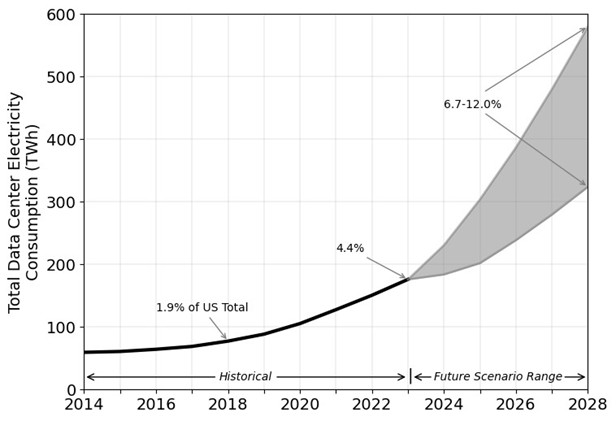
\includegraphics[width=.8\linewidth]{Figures/Data Center Electricity Consumption over Time (1).jpg}
    \caption{Projected data center growth over time. Source: DOE.}
    \label{fig:DataCenterGrowth}
    \vspace{-10pt}
\end{wrapfigure}
 
Over the past six years, data centers have expanded from consuming 1.9\% to 4.4\% of total U.S.\ electricity demand (Figure~\ref{fig:DataCenterGrowth}, DOE). This rapid growth---driven largely by artificial intelligence---follows two decades of essentially flat electricity consumption and coincides with nationwide efforts to electrify transport and heating. Grid infrastructure was planned for stable demand, not simultaneous load growth from multiple sectors. The combination raises fundamental questions about how AI-driven electricity demand affects reliability, prices, and emissions---and whether the procurement instruments that hyperscalers use to meet voluntary clean energy commitments are adequate to address these externalities.
 
Data center hyperscalers have responded to scrutiny over their growing electricity footprint by purchasing renewable energy certificates (RECs) and signing power purchase agreements (PPAs), often claiming carbon-neutral or ``100\% renewable'' operations on this basis. Yet the economics of these instruments suggest reasons for skepticism. RECs are financial transfers that do not alter real-time dispatch; a hyperscaler that retires RECs on an annual basis may still draw power from fossil generators during every hour of peak demand. PPAs contract for renewable output but do not guarantee temporal alignment between generation and consumption. Whether these instruments meaningfully reduce the grid-level externalities of AI workloads---or primarily serve as accounting devices---is an open empirical question with significant policy implications.
 
Our paper makes two contributions to address it. First, we develop a game-theoretic model of hyperscaler electricity procurement in which a large data center operator chooses between RECs, PPAs, and behind-the-meter colocation, while generators make entry decisions under endogenous financing costs. The model yields sharp predictions. Because renewable generation is intermittent, incremental data center demand raises fossil generation---and therefore emissions and prices---unless storage or colocation can shift clean energy into the hours when load is highest. We formalize this as the \emph{timing wedge}: the gap between when a hyperscaler consumes electricity and when its contracted or credited renewable generation actually produces. REC purchases do not shrink this wedge in the short run; PPAs reduce it only modestly absent firming; colocation with storage addresses it directly by physically supplying the data center with renewable energy in real time. The model further predicts an investment hierarchy driven by financing risk: colocation eliminates revenue variance for generators and therefore induces the greatest renewable entry, followed by PPAs, then merchant REC arrangements. The paradoxical implication is that even a hyperscaler purchasing RECs to cover 100\% of its annual load can simultaneously degrade local reliability, raise wholesale prices, and increase system-wide emissions. Colocation with storage and generation substantially mitigates these outcomes.
 
Second, we provide the first causal estimates of these grid-level externalities. Exploiting the staggered release of frontier large language models (LLMs) as a natural experiment, we use difference-in-differences methods to estimate how AI model training and inference affect local power quality, fossil fuel generation, and wholesale electricity prices. The empirical results are consistent with the model's predictions. We find that large model releases cause significant power quality deterioration---well above half the standard deviation of U.S.\ power quality distributions---and increase fossil fuel consumption on the order of hundreds of GWh during both training and inference phases. Wholesale electricity prices increase substantially in treated zones, with increases of up to 25\% in the American Electric Power (AEP) zone of PJM. Critically, we find that data centers with on-site generation exhibit a sign reversal in power quality effects relative to those without, consistent with the model's prediction that behind-the-meter generation absorbs demand spikes that would otherwise propagate to the grid. Impact magnitudes scale with model size, suggesting that these externalities will grow as frontier models continue to expand.
 
Our theoretical and empirical analyses jointly speak to an active policy debate. Proposals for hourly renewable matching---such as those advanced under the 24/7 Carbon-Free Energy framework---attempt to close the timing wedge by requiring temporal alignment of clean energy credits with consumption. Our model provides a framework for evaluating such proposals: tightening the granularity parameter $h$ raises effective REC prices in high-carbon hours and increases the private value of storage and temporally aligned generation, shrinking the timing wedge in equilibrium through both entry and operational responses. We complement the model's comparative statics with descriptive analysis of REC and PPA markets, documenting the gap between contracted clean energy and real-time grid conditions that gives rise to the timing wedge in practice.
 
The paper also contributes methodologically. Because proprietary operational data on AI workloads are unavailable, we construct a novel dataset linking publicly available power grid data, data center locations, AI model release dates, and market prices. We use publicly announced model training and release dates as plausibly exogenous shocks and apply staggered difference-in-differences estimation \citep{cengiz2019effect, deshpande2019screened} to address variation in treatment timing across models and locations. We validate our identification strategy through parallel trends tests, placebo exercises with randomized treatment dates and locations, alternative geographic boundary definitions, and time series anomaly detection. To address supply-side confounds in the fossil fuel demand analysis, we instrument for electricity prices using the interaction of generator-level heat rates and regional natural gas prices.
 
This work connects four literatures. It contributes to the economics of electricity markets by documenting a new and rapidly growing source of demand-side pressure on wholesale prices and grid reliability \citep{borenstein2002trouble, joskow2008capacity}. It advances the literature on environmental externalities from industrial electricity consumption \citep{fowlie2012industrial, greenstone2014environmental} by showing that voluntary procurement instruments may fail to internalize the externalities they are designed to address. It engages the emerging literature on the energy and environmental footprint of AI \citep{strubell19, schwartz2020green, morrison2025holistically} by moving from facility-level accounting to system-level causal estimation. Finally, it informs the policy debate over renewable energy procurement design \citep{miller2022hourly} by providing both a theoretical framework and empirical evidence for evaluating alternative matching granularities.
 
The remainder of the chapter proceeds as follows. Section~\ref{sec:relatedwork} reviews related work. Section~\ref{sec:model} presents the game-theoretic model, including the toy model that illustrates core mechanisms and the full model with equilibrium characterization. Section~\ref{sec:empirical} describes the empirical setting, data construction, and econometric methodology. Section~\ref{Sec::Results} presents estimation results. Section~\ref{sec:counterfactuals} reports counterfactual analyses examining alternative AI development trajectories. Section~\ref{sec:conclusion_aipower} concludes.

\section{Related Work}\label{sec:relatedwork}

This paper contributes to four interrelated economics literatures: wholesale electricity market design, environmental externalities from industrial electricity consumption, renewable energy procurement and corporate carbon accounting, and the emerging empirical literature on data center grid impacts.
 
\subsection{Wholesale Electricity Markets and Demand Shocks}
 
The institutional foundations of U.S. wholesale electricity markets are well established. \citet{borenstein_bushnell2015} provide a comprehensive assessment of restructuring outcomes, documenting that wholesale price formation via locational marginal pricing remains sensitive to demand conditions due to the convex shape of the aggregate supply curve and limited short-run demand elasticity \citep{borenstein2002trouble}. In this setting, large demand increases---such as those from data center load---move clearing prices up the supply curve and may amplify market power rents \citep{borenstein2002measuring, borenstein_bushnell1999}. \citet{bushnell_mansur_saravia2008} show that vertical arrangements and forward contracting dramatically affect wholesale prices in restructured markets, a finding relevant to the bilateral power purchase agreements increasingly used by hyperscalers.
 
Transmission constraints further shape how demand shocks propagate. \citet{borenstein_bushnell_stoft2000} analyze how limited transmission capacity creates localized price effects---precisely the mechanism through which geographically concentrated data center load elevates LMPs in constrained corridors. \citet{joskow2008capacity} identifies the ``missing money'' problem in capacity markets, directly relevant as PJM capacity prices rose from \$30 to \$270/MW-day between 2023 and 2024, partly driven by data center growth \citep{cmu2025}. \citet{joskow2019} further documents how intermittent renewable generation complicates wholesale market investment signals, a challenge amplified when new baseload demand from data centers coincides with coal retirements and renewable expansion.
 
The merit-order literature provides the inverse mechanism to our analysis. While \citet{sensfuss2008} and \citet{cludius2014} show that zero-marginal-cost renewables shift supply rightward and depress wholesale prices, data center demand shifts demand rightward, moving clearing prices up the supply curve. This symmetry motivates our focus on wholesale price effects as a primary outcome.
 
\subsection{Environmental Externalities and Marginal Emissions}
 
A large literature documents how industrial electricity consumption generates environmental externalities that vary dramatically by location and time. \citet{siler_evans2012} provide the first systematic calculation of marginal emissions factors for the U.S. grid, revealing substantial regional variation. \citet{graff_zivin2014} extend this framework to show more than threefold variation in marginal emissions across regions, with direct implications for evaluating how data center siting decisions affect net emissions. \citet{holland2022pnas} demonstrate that despite declining \emph{average} grid emissions, \emph{marginal} CO$_2$ emissions from U.S. electricity generation have not decreased---a critical finding for assessing the true environmental impact of incremental data center demand. \citet{callaway_fowlie2018} quantify how the location of demand reduction or renewable generation affects emissions displacement, directly relevant to data center siting.
 
The emissions leakage literature provides further context. \citet{fowlie2009} shows that incomplete cap-and-trade regulation achieves only a fraction of intended emissions reductions due to leakage across jurisdictional boundaries. \citet{fell_maniloff2018} provide empirical evidence that RGGI caused coal generation to shift to non-participating states. These mechanisms are directly applicable to data centers: load growth in one region can increase fossil fuel dispatch in neighboring regions, undermining the environmental benefits of local renewable procurement. \citet{holland2016aer} demonstrate that externalities from electricity-intensive activities in one state are substantially exported to others via the interconnected grid.
 
\subsection{Renewable Energy Certificates and Corporate Procurement}
 
A growing literature evaluates the environmental effectiveness of corporate clean energy procurement strategies. \citet{gillenwater2008a} establishes that unbundled RECs fail credible additionality tests, and \citet{gillenwater2014} shows empirically that the voluntary REC market has negligible influence on the economic feasibility of new wind projects. \citet{bjorn2022} find that when REC-based emission reductions are removed from corporate inventories, companies' scope~2 trajectories no longer align with climate targets. \citet{brander2018} identify fundamental problems with the GHG Protocol's market-based method that allows hyperscalers to claim zero scope~2 emissions via REC purchases.
 
System-level modeling confirms this hierarchy. \citet{xu2024} provide the first comprehensive comparison of annual volumetric matching, hourly (24/7) matching, and emissions-based matching strategies, finding that annual matching via RECs does little to reduce system-level emissions while hourly matching is significantly more effective. \citet{riepin2024} find similar results in European markets, estimating that 98\% hourly carbon-free energy matching carries a 54\% cost premium over annual matching but substantially reduces system emissions. On the PPA side, \citet{backstrom2023} use U.S.\ county-level data with two-way fixed effects to show that corporate PPAs have influenced aggregate renewable capacity---unlike voluntary RECs---though effects are heterogeneous across contract types and regions.
 
These findings motivate our game-theoretic procurement model. The empirical literature establishes a clear hierarchy of environmental effectiveness---unbundled RECs (lowest), annual volumetric matching, and 24/7 hourly matching (highest)---that maps onto the strategic choices available to hyperscalers in our framework.
 
\subsection{Data Center Grid Impacts}
 
Our paper contributes most directly to the emerging empirical literature on data center electricity market impacts. \citet{benetton2023} establish the template for studying how large, geographically concentrated computing loads create electricity price externalities: using Bitcoin price as an exogenous demand shifter in Upstate New York, they find that cryptocurrency mining raised electricity costs by \$92 million annually for small businesses and \$204 million for households. We extend this approach to AI-driven data center demand, using model releases rather than cryptocurrency prices as the demand shock.
 
Several concurrent papers study data center grid impacts using complementary methods. \citet{mamkhezri2025} use difference-in-differences examining Virginia data center expansion on wholesale prices across census tracts, finding that interconnections raise wholesale prices by 7.3\% through congestion and marginal loss components. \citet{kay2026} develop an hourly least-cost dispatch model covering all U.S.\ wholesale markets, finding existing data centers have increased wholesale prices by 3--5\% nationally, with substantially larger effects in data center corridors and projected increases of 20--50\% under high-utilization scenarios. \citet{bogmans2025} use a multi-country CGE model to project U.S.\ electricity price increases of 8.6\% and carbon emissions increases of 5.5\% from AI-driven data center growth. \citet{knittel2025} model data center flexibility in PJM, ERCOT, and WECC, finding that flexible scheduling reduces system costs but has ambiguous emissions effects depending on the generation mix.
 
On the political economy side, \citet{gargano2025} study state-level tax incentives for data centers using staggered DiD, finding that incentives increase development but with limited employment impacts. \citet{jacobs2025} documents \$4.3 billion in transmission connection costs passed to PJM ratepayers.
 
Our paper differs from this literature in three respects. First, our game-theoretic procurement model connects the empirical findings on price and emissions externalities to the strategic incentives facing hyperscalers, bridging the gap between the market impact and corporate procurement literatures. Second, we use AI model releases as plausibly exogenous demand shocks, providing an identification strategy that does not rely on observing facility-level capacity additions. Third, we examine power quality degradation alongside price effects, capturing externalities beyond the wholesale market.
 

\section{Industry Background}
% % \nb{One possibility is to roll this in with the problem definition in 3.1 if we need space.}
% % \nb{We should also have related work in terms of what kinds of analysis has been done and explain what our work contributes hasnt been done or not easily inferrable from existing work.}
U.S. data centers are expanding rapidly, nearly tripling from its 2008 levels to 1489 active sites in 2025, with another 1,359 on the horizon~\cite{aterio_us_data_centers_2025}. The market is dominated by \emph{hyperscalers}---vertically integrated data centers---owned by AI heavy companies such as Amazon, Microsoft, and Google, alongside a long tail of smaller operators. Hyperscalers afford companies certain economies of scale but greatly increase the geographic concentration of power demand on the grids. Concentrated demand strains local grids in the area, raising congestion costs and sometimes degrading power quality for neighboring consumers. Large, inflexible loads from AI hyperscalers also reduce system reliability, elevate wholesale prices, and complicate renewable integration.
\subsection{Market Overview}

The U.S. data center market has expanded rapidly, growing from 519 facilities in 2008 to 1,489 active sites in 2025, with another 1,359 announced or under construction \cite{aterio_us_data_centers_2025}. Electricity demand more than tripled over this period, rising from under 5 to over 15 GWh per hour (BNEF), while total U.S. capacity increased only 17.6\% \cite{EIA_2023_table4_2A} and dispatchable baseload capacity fell as coal retired.
Power consumption has risen in parallel, though since 2018 growth in renewable generation has outpaced data center demand as shown in Figure \ref{fig:DCPowerConsumption}.

\begin{wrapfigure}{l}{0.45\linewidth}
    \centering
    \vspace{-10pt}
    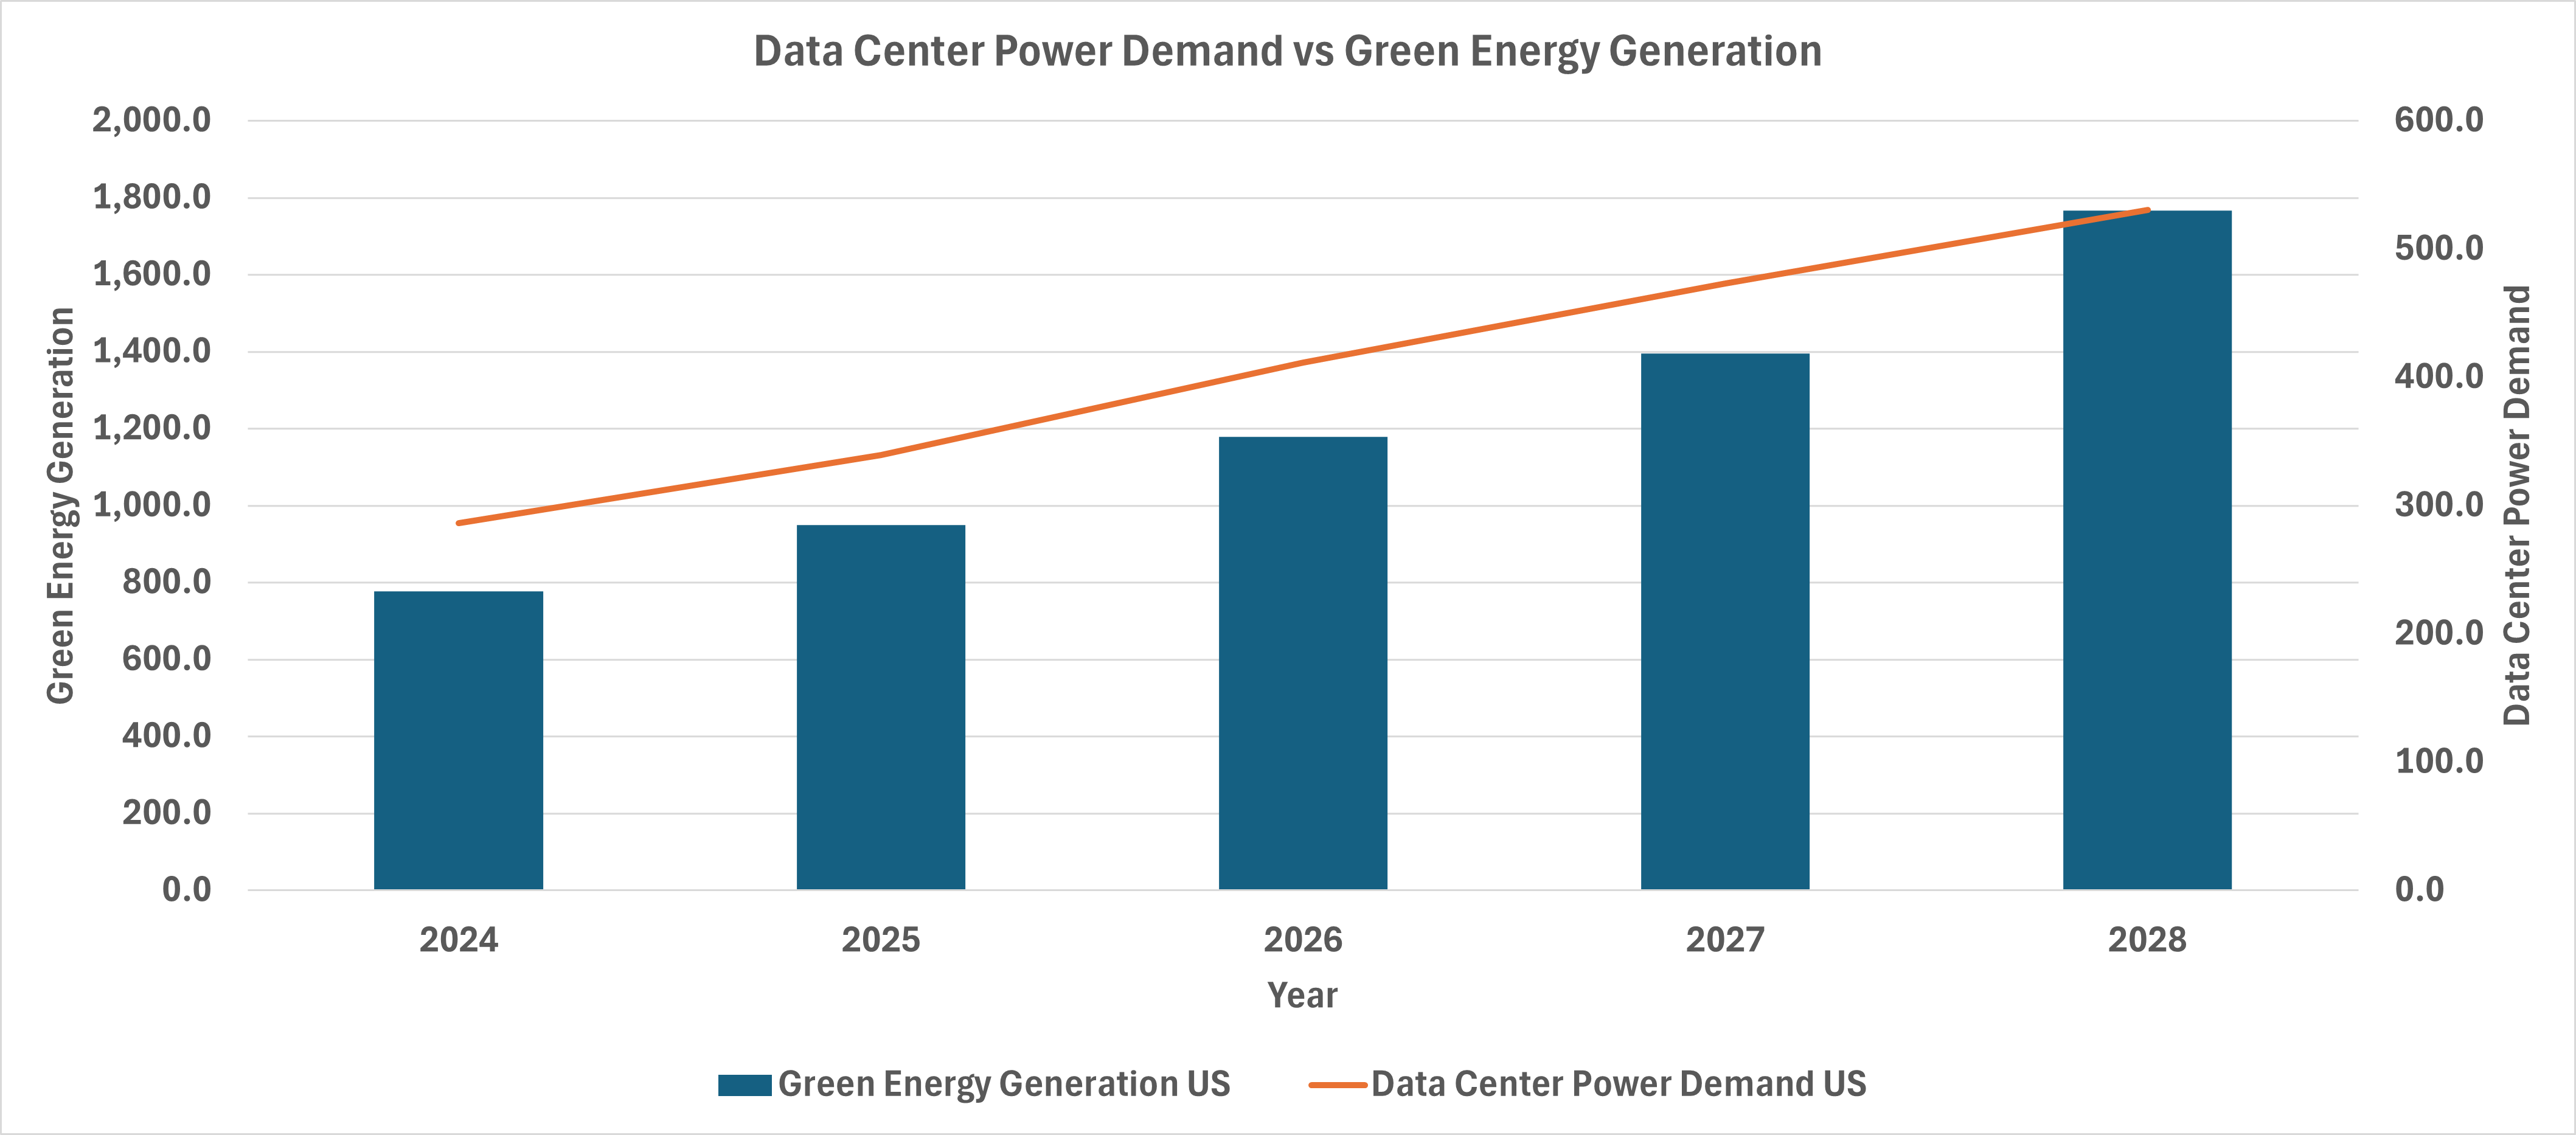
\includegraphics[width=\linewidth]{Figures/Data Center Power Demand vs Green Generation.png}
    \caption{Data center power consumption vs.\ green generation. Source: Aterio.io.}
    \label{fig:DCPowerConsumption}
    \vspace{-10pt}
\end{wrapfigure}

The market is geographically concentrated and dominated by hyperscalers—Amazon, Microsoft, and Google—who account for 38\% of capacity across five firms, and 64\% across twenty. Unlike colocation providers such as Equinix, hyperscalers are vertically integrated, owning facilities, long-term power contracts, fiber networks, and custom chips.


\begin{figure}[t!]
    \centering
    % First figure
    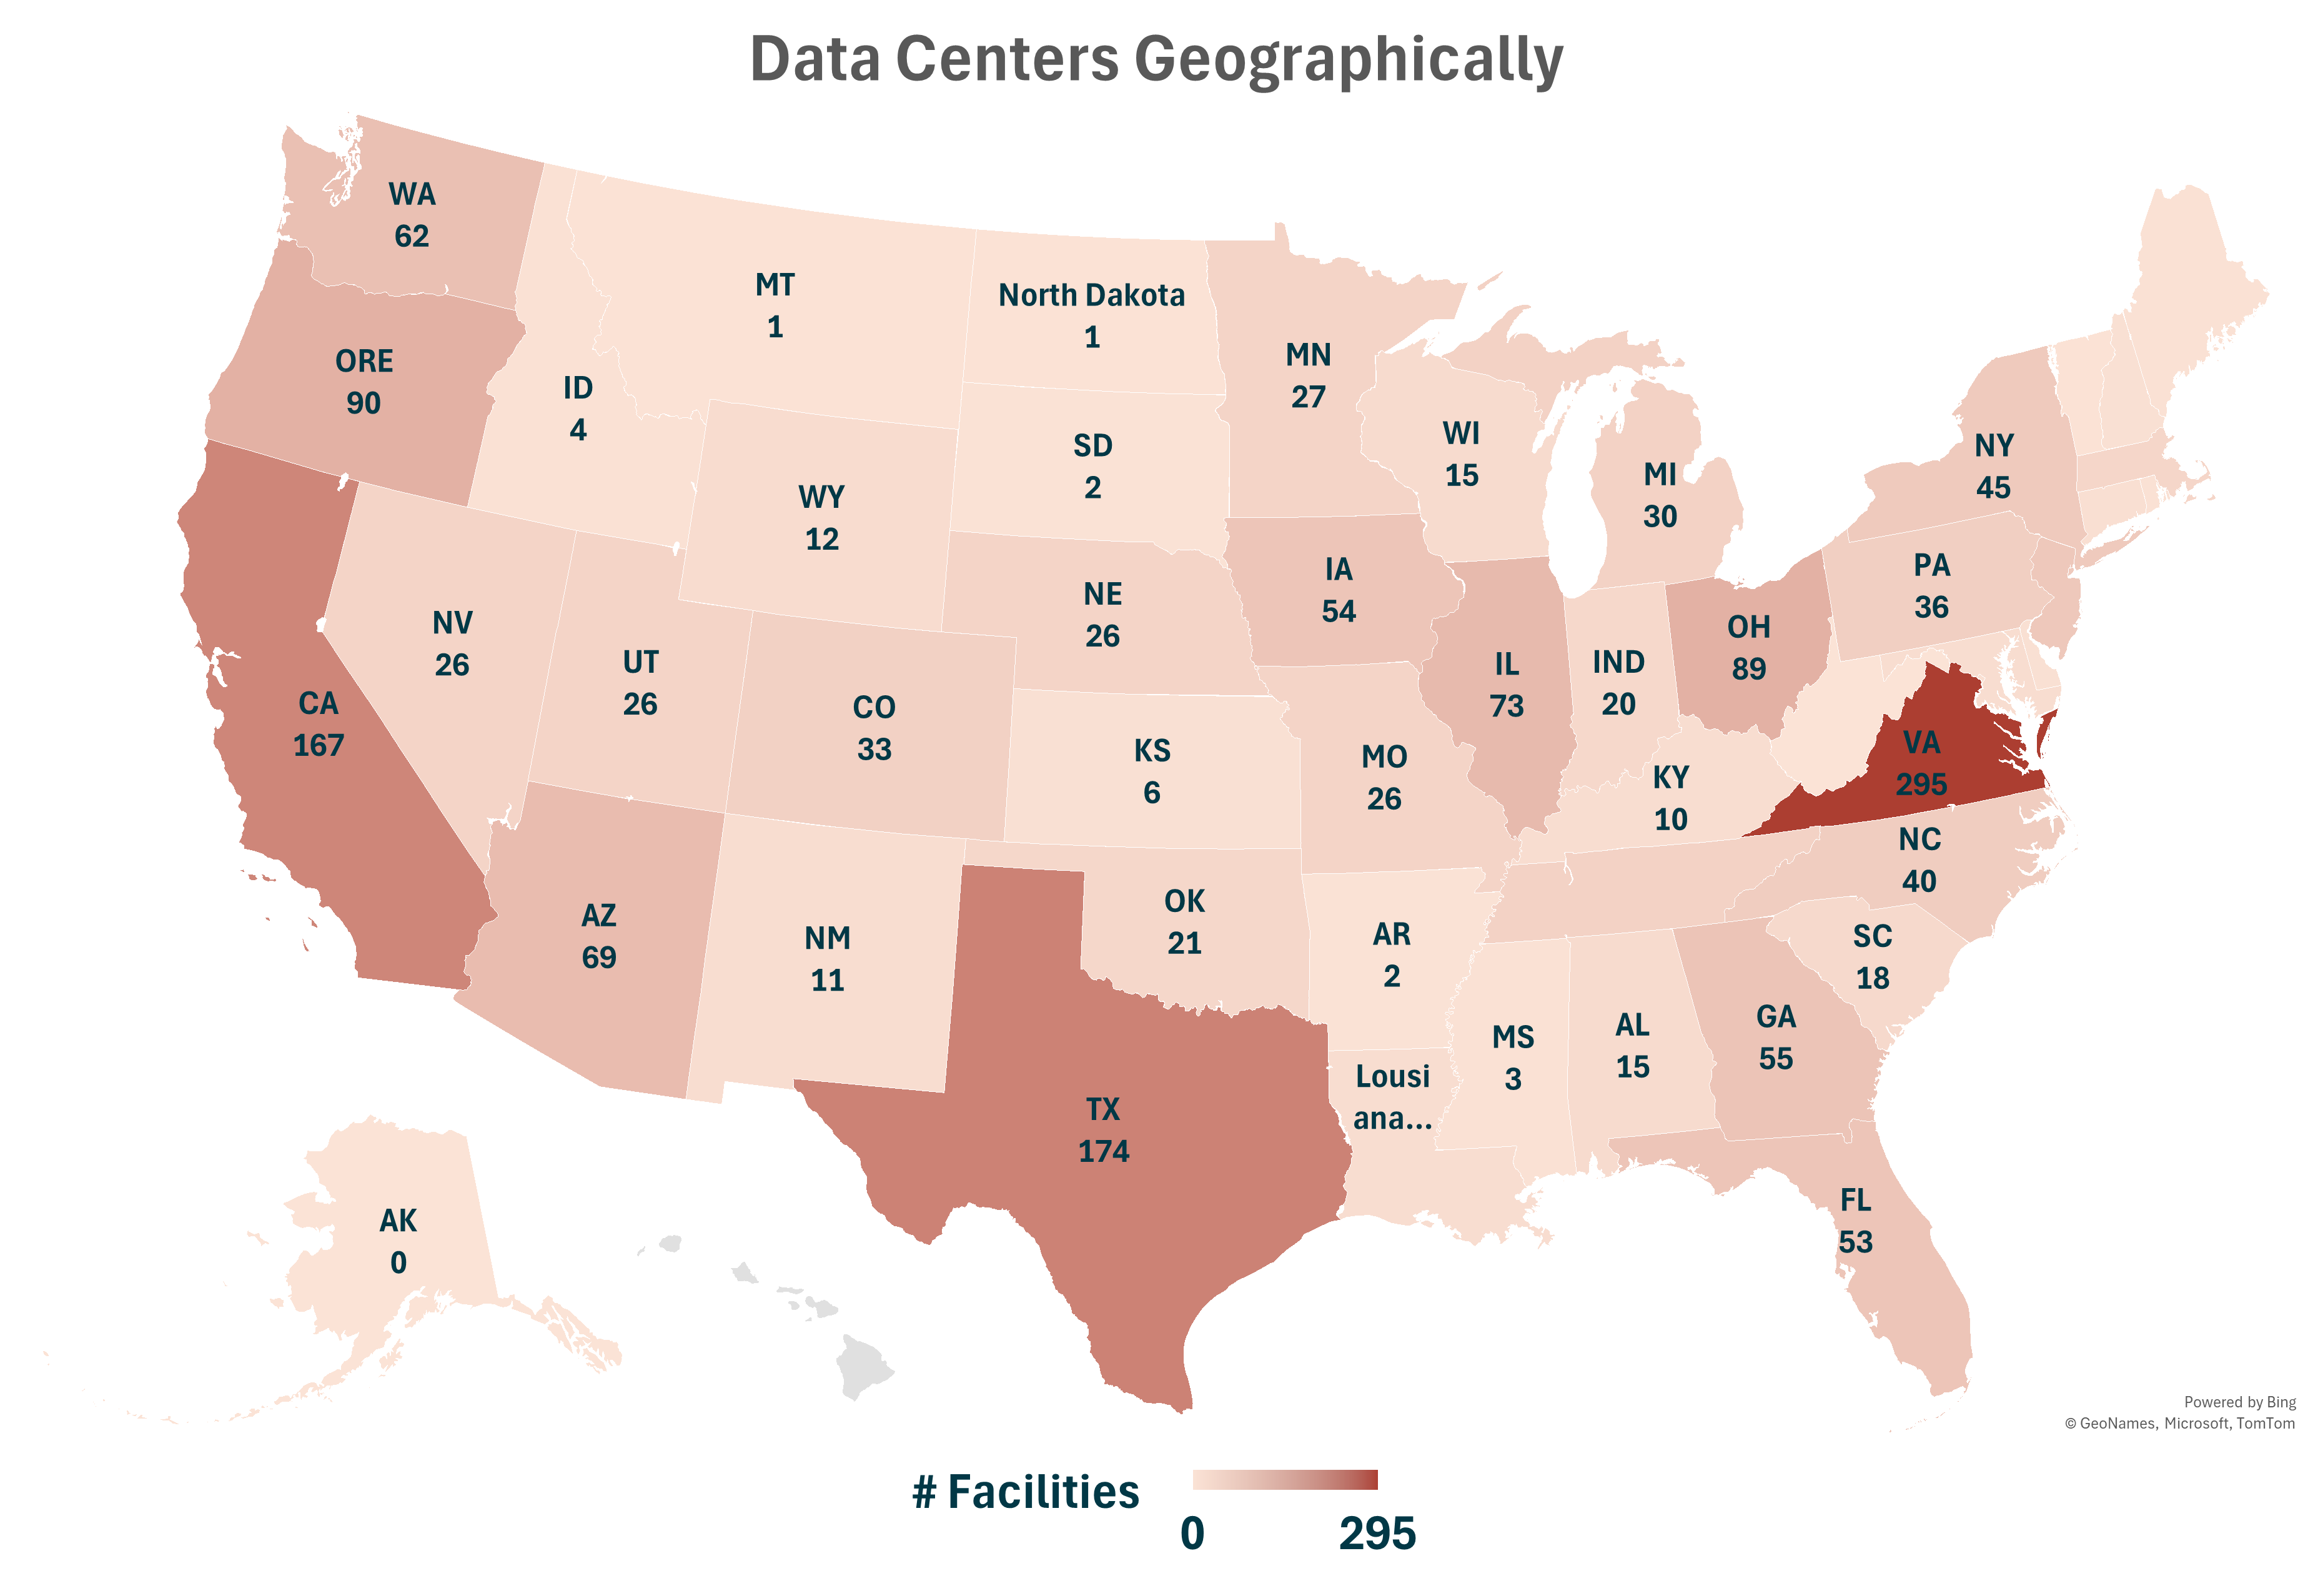
\includegraphics[width=\linewidth]{Figures/Data Centers by State.png}
        \caption{Data centers by state. Source: Aterio.io.}
        \label{fig:DCbyState}
\end{figure}

These economies of scale, however, generate externalities. Concentrated demand in specific regions strains local grids, raising congestion costs and sometimes degrading power quality for neighboring consumers. Large, inflexible loads reduce system reliability, elevate wholesale prices, and complicate renewable integration. At the same time, clustering provides local benefits through jobs, tax revenues, and downstream services. Data centers thus act as both efficiency drivers and sources of regional externalities. It is important to consider the mitigation of the externalities to the grid when analyzing the impacts of AI. We focus on hyperscalers in our paper because hyperscalers perform the majority of AI training and also because larger facilities are more likely to cause power distortions.
% \aruna{Is there a reason why we are talking about hyperscalers? Should we say therefore we focus on these hyperscalers?}

The industry is also geographically concentrated. Texas, California, and especially Virginia dominate U.S. capacity. Virginia’s cluster reflects historic federal investments in internet infrastructure and the routing of early traffic through Northern Virginia. More recent growth in Texas stems from lower electricity costs and streamlined permitting.

The electricity market includes three separate components: generation, transmission, and distribution. Generation is how power is produced. Transmission involves long-range transportation of electricity while distribution involves local distribution of electricity. In the United States, there are two primary models of how the electricity market is structured: vertically integrated utilities and deregulated markets. In vertically integrated utilities, which are prevalent in the South and West, generation, distribution, and transmission are all owned and operated by one company whereas in deregulated markets generation bids in wholesale markets to provide power to utilities, which own transmission and distribution, and provide power in the retail markets. Figure \ref{fig:ISOMap} provides a map showing the geographic makeup of the American electricity market.

\begin{figure}
    \centering
    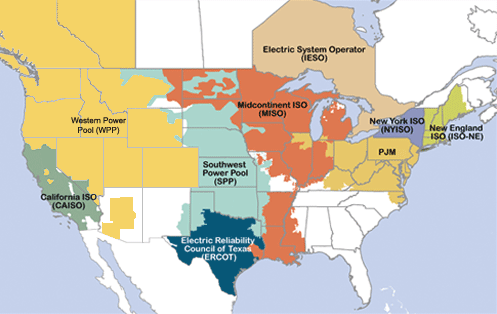
\includegraphics[width=0.5\linewidth]{Figures/ISOMap.png}
    \caption{Map of American electricity market.}
    \label{fig:ISOMap}
\end{figure}

These dynamics interact with broader shifts in the electricity market: greater electrification and the transition from fossil fuels to renewables. Because renewables are intermittent and less dispatchable, rising data center loads coupled with greater renewable penetration place dual pressures on grids, shaping both market outcomes and policy debates. It is therefore crucial to quantify how much power AI uses, how it distorts quality and impacts prices, and the role of efficiency improvements and developments in computing.

% \subsection{Total Harmonic Distortion}
\begin{wrapfigure}{r}{0.3\linewidth}
    \centering
    \vspace{-18pt}
    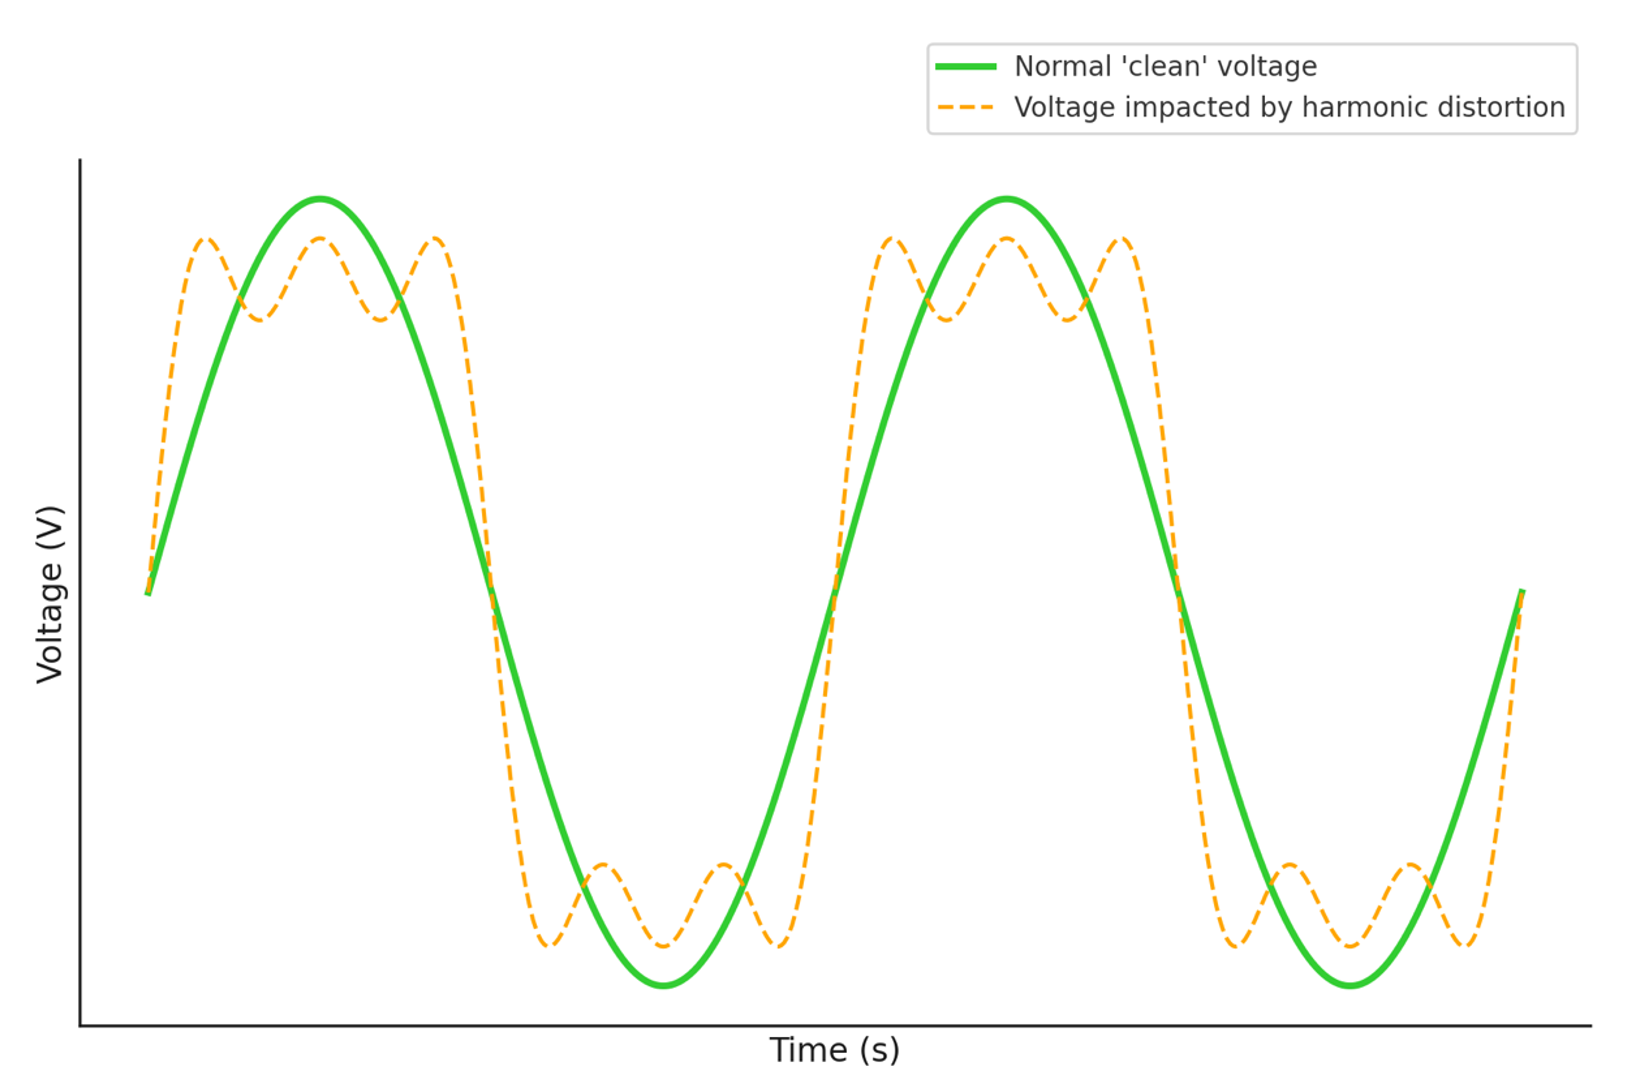
\includegraphics[width=\linewidth]{Figures/HarmonicDistortion.png}
    \caption{Total harmonic distortion representation.}%\aruna{this figure is not referenced in the text}}        
    \label{fig:THD}
    \vspace{5pt}
\end{wrapfigure}
% Figure~\ref{fig:THD} illustrates the distortions in the power frequencies. The green line shows the \emph{clear} voltage curve, which is cleanly sinusoidal, whereas with huge loads can produce harmonic distortions shown as the dotted yellow curve. This \emph{dirtier} voltage can adversely affect the operation and lifetime of household appliances and other products that use electricity.

\subsection{Background: Data Center Concentration and Power-Quality}

AI workloads affect power quality through three main mechanisms. First, data centers and AI computing facilities add substantial baseload demand that can strain grid capacity and compromise voltage regulation, especially during peak periods. Second, AI workloads fluctuate rapidly with computational needs, creating unpredictable load variations that challenge stability and frequency regulation. Third, the switching power supplies and electronics essential to AI hardware generate harmonic distortion, introducing waveform distortions that spread through distribution networks and degrade power quality. Figure~\ref{fig:THD} illustrates the distortions in the power frequencies. The green line shows the \emph{clear} voltage curve, which is cleanly sinusoidal, whereas with huge loads can produce harmonic distortions shown as the dotted yellow curve. This \emph{dirtier} voltage can adversely affect the operation and lifetime of household appliances and other products that use electricity.

\begin{wrapfigure}{r}{0.3\linewidth}
    \centering
    \vspace{-18pt}
    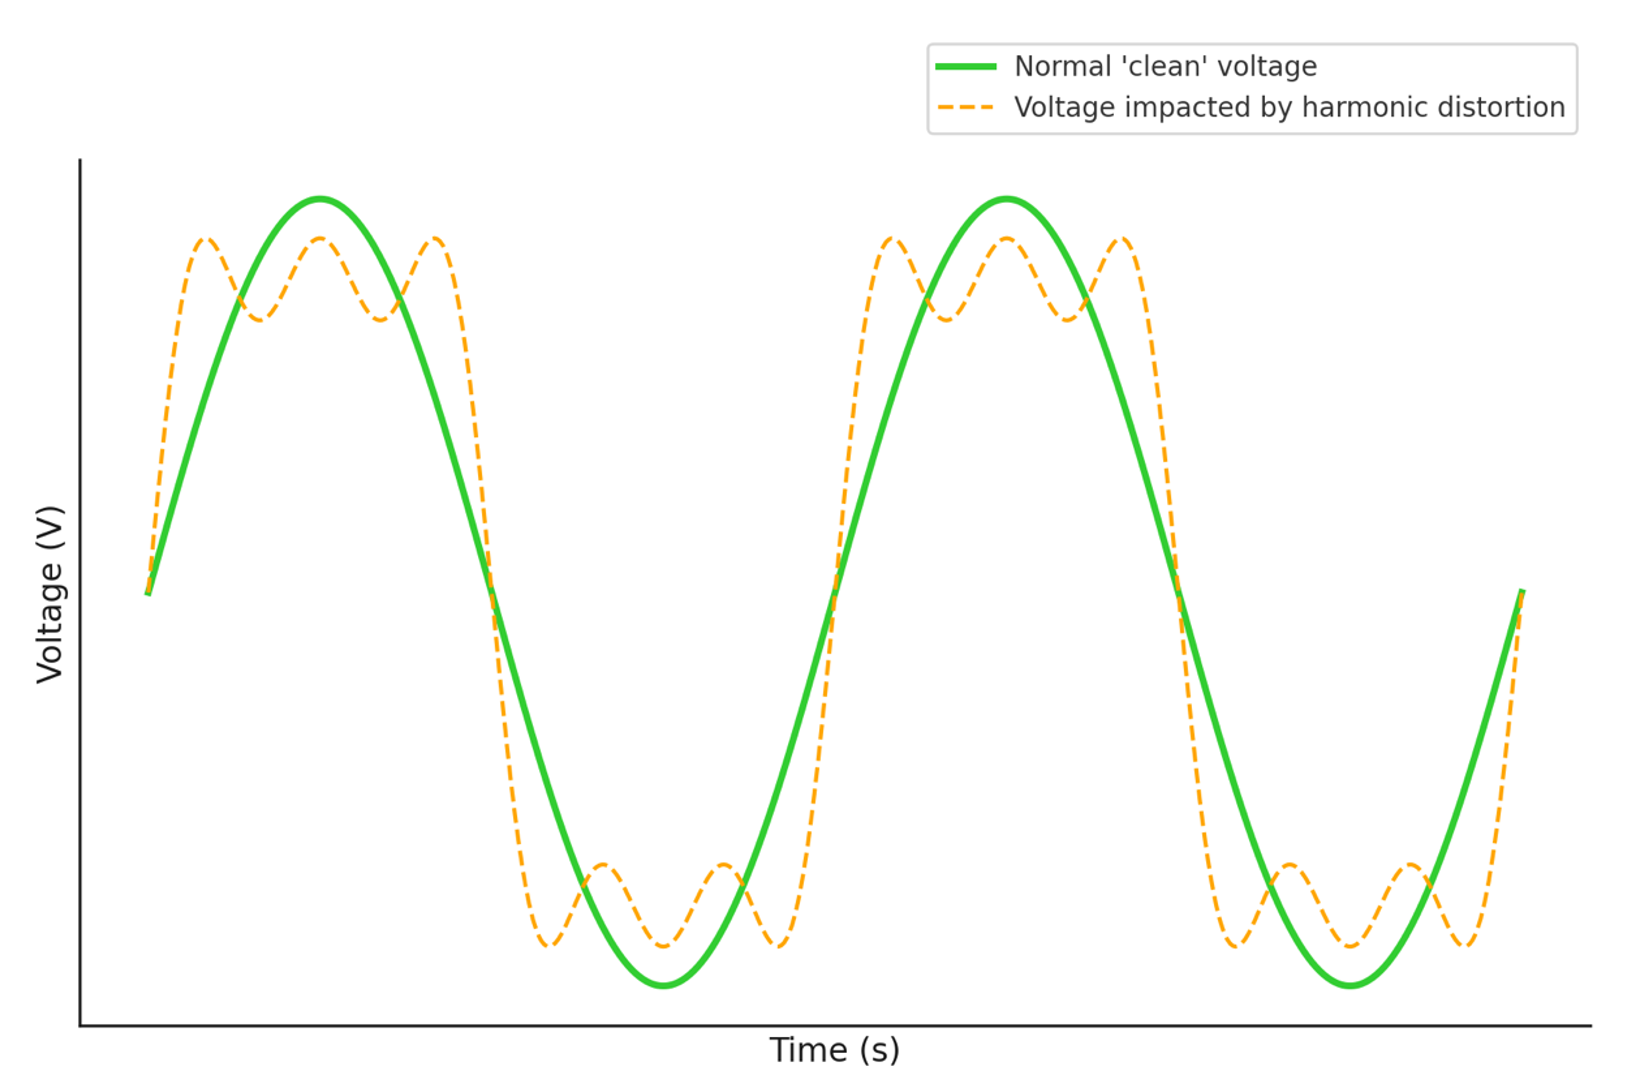
\includegraphics[width=\linewidth]{Figures/HarmonicDistortion.png}
    \caption{Total harmonic distortion representation.}%\aruna{this figure is not referenced in the text}}        
    \label{fig:THD}
    \vspace{5pt}
\end{wrapfigure}

AI workloads also affect wholesale electricity prices through the demand channel, with potentially indeterminate long-run retail market impacts. The U.S. electricity sector comprises both vertically integrated utilities and restructured markets featuring competitive wholesale generation alongside monopoly retail distribution. Wholesale prices are determined hourly in day-ahead markets via sealed-bid, uniform-price auctions subject to network constraints. Locational price variation reflects transmission limitations within the network. Increased demand raises wholesale prices by necessitating dispatch of higher-cost marginal generators.

Wholesale prices are passed through to retail consumers with substantial lag. Retail rates typically reflect average procurement and distribution costs plus a state-regulated return on investment, calculated from historical data. This passthrough mechanism is indirect even absent investment-related dynamics. While new demand sources could theoretically dilute system-wide fixed costs and reduce average retail prices, increased demand more likely raises retail rates. Understanding wholesale demand and price shifts thus provides useful intuition regarding the direction and magnitude of retail price changes.

\subsection{RECs, PPAs, and Colocation}
Corporate electricity procurement takes several forms. Each procurement option entails distinct implications for grid externalities. The most common method is direct procurement, in which a facility draws power as a standard load-serving customer, inheriting the emissions profile of the local generation mix. Often but with increasing rarity and due to the structure of the market, data centers participate directly in the retail electricity market and only interact with utilities.

Despite purchases of electricity with the same properties of that delivered to all other buyers, many hyperscalers claim that they use only renewable electricity. How can this be? To claim renewable attributes without altering physical electron flows, many data center operators purchase renewable energy certificates (RECs). RECs unbundle the environmental attributes of renewable generation into tradeable commodities representing one MWh of renewable output. RECs originated as compliance instruments for state renewable portfolio standards \citep{epa_rec_definition,wiser2004alternative}. REC markets are regulated at the local level with differing standards across markets. Some markets require retirement of RECs in the same geographic market to count. A data center in PJM cannot retire RECs from an ERCOT wind farm. However, this is mostly statutory and is less impactful for voluntary REC purchases. Other markets include voluntary purchases that impose no spatial or temporal constraints.  This disconnect underlies the ``timing wedge'' identified in this paper—annual 100\% renewable claims coexisting with fossil-heavy consumption during peak hours. Empirical evidence suggests the emissions-reduction value of unbundled RECs may be near zero in many markets \citep{bjorn2022recs,gillenwater2007recs}.

Power purchase agreements (PPAs) offer a closer link between procurement and consumption. As shown in Figure \ref{fig:PPAFigure}, PPAs by data centers have risen precipitously since 2016 and have grown alongside data center power consumption. While most PPAs were historically wind-based, battery and solar PPAs are increasingly common, and nuclear PPAs are emerging as a favorite of industry leaders. Physical PPAs deliver contracted renewable power to the offtaker's node, while virtual (financial) PPAs provide contract-for-differences settlements without physical delivery, sharing the spatial mismatch limitations of unbundled RECs. The key distinction is whether procurement induces \textit{incremental} renewable capacity that is \textit{deliverable} to the relevant node \citep{taheri2025ppa,kobus2021ppa}.

\begin{figure}
    \centering
    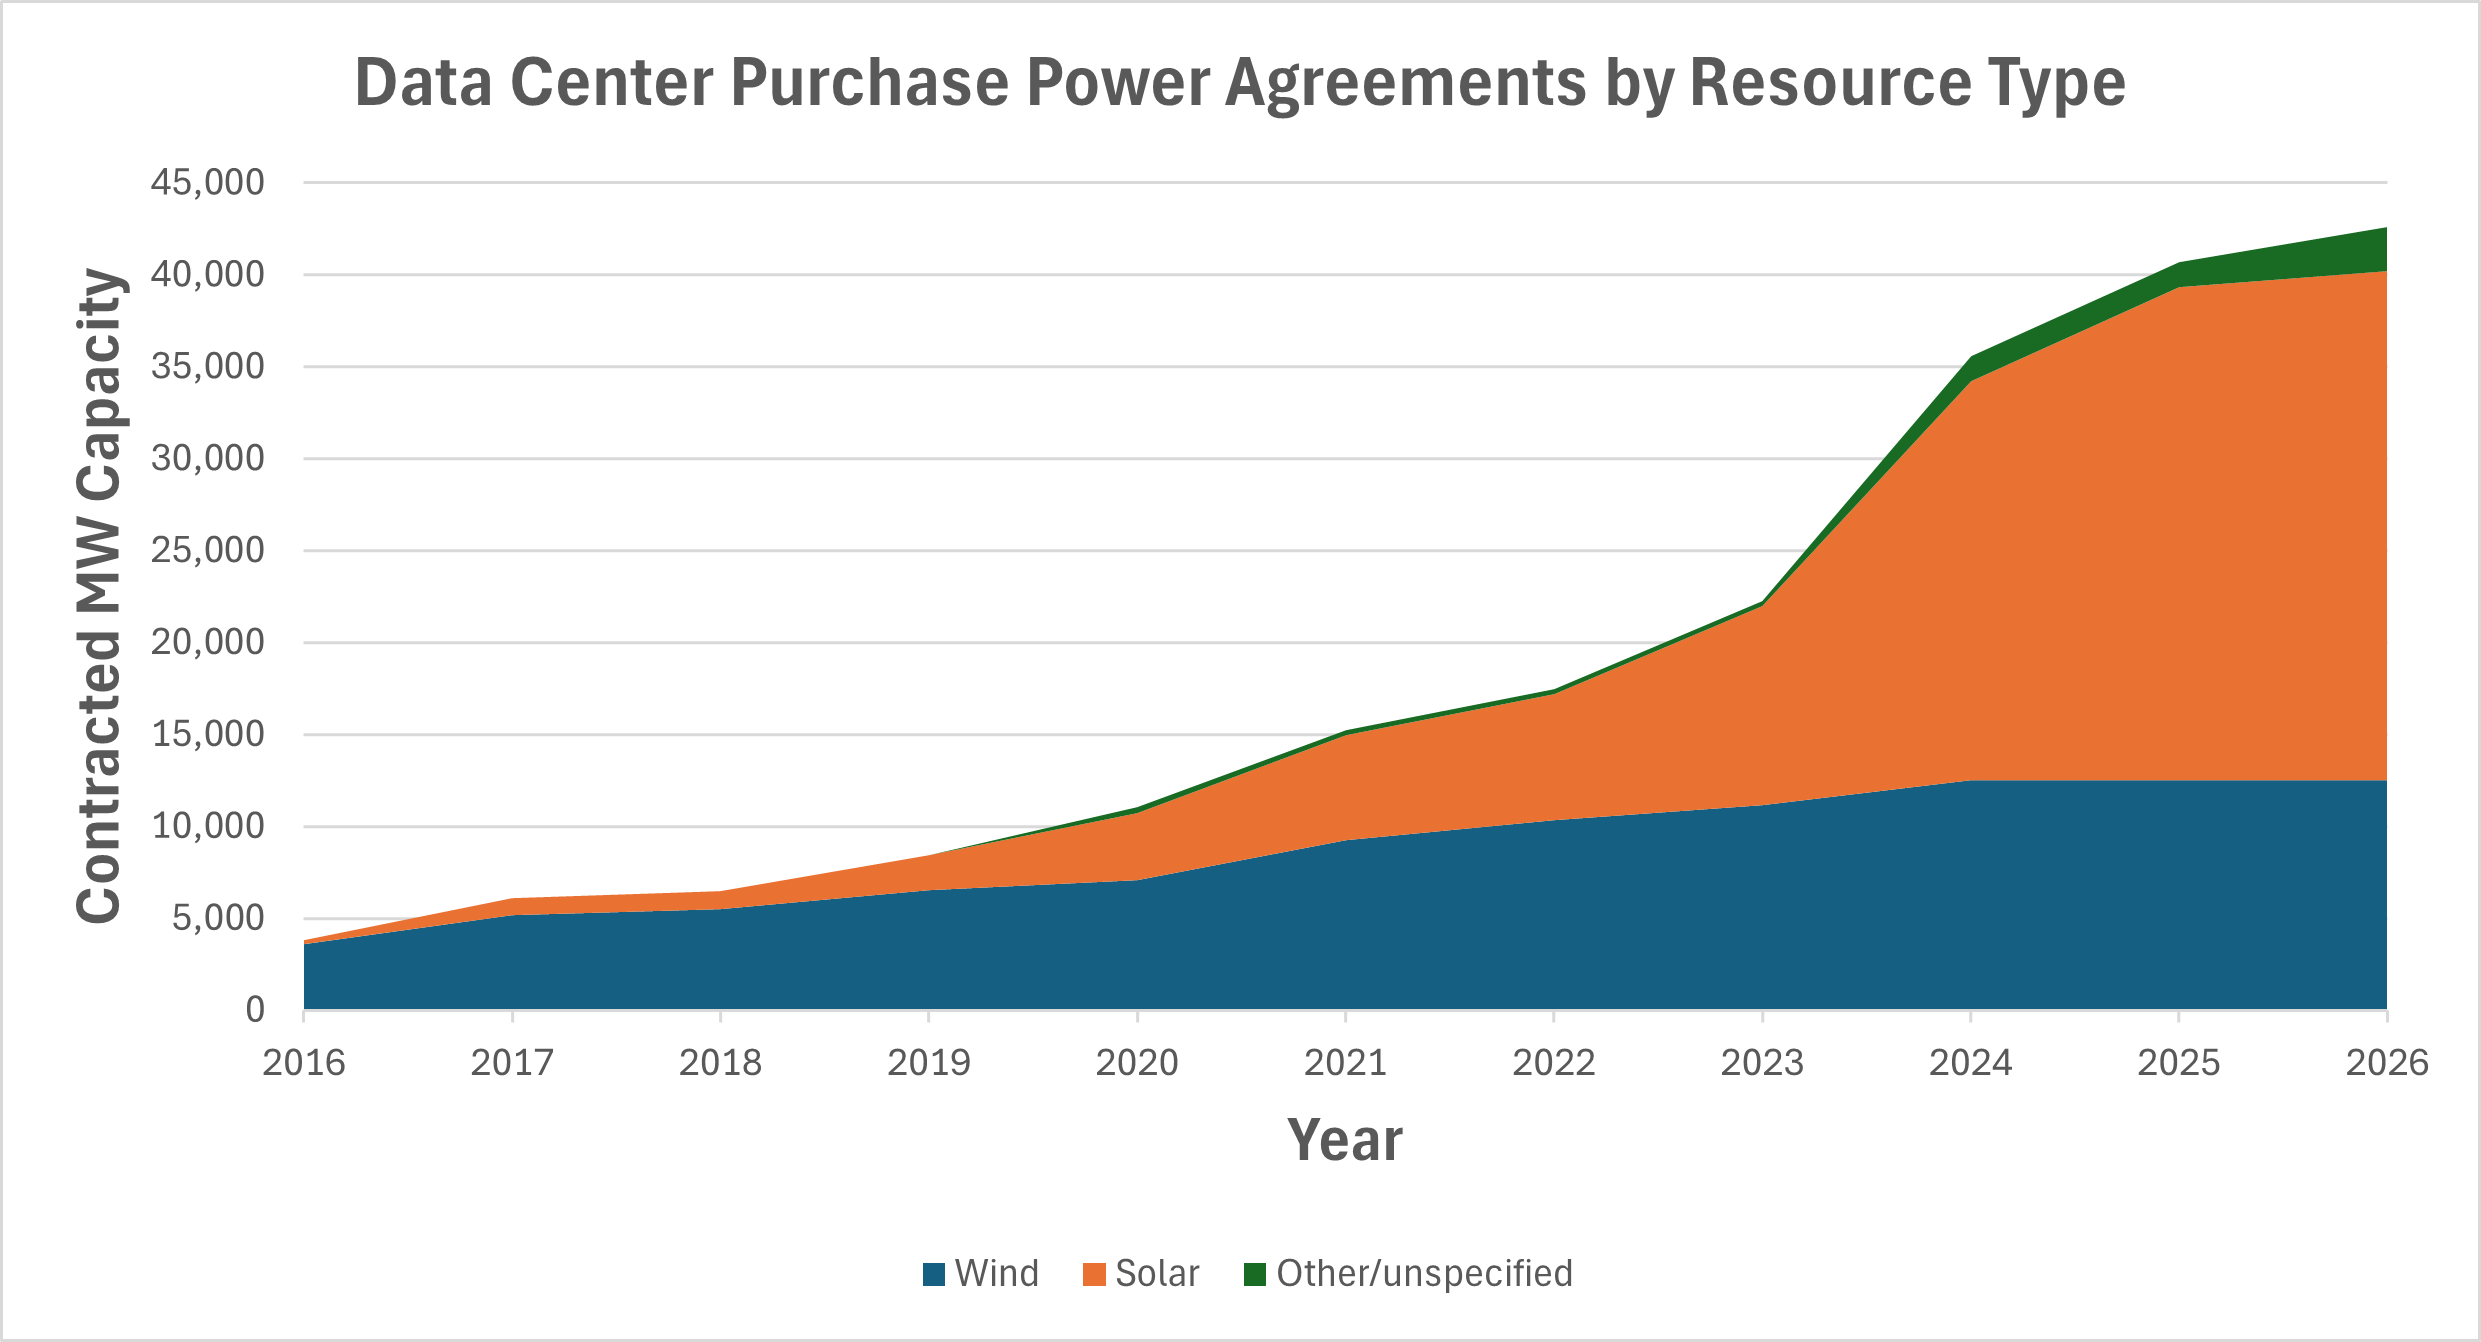
\includegraphics[width=0.5\linewidth]{Figures/PPA by Resource Type.png}
    \caption{PPA agreements by data centers have risen dramatically since 2016.}
    \label{fig:PPAFigure}
\end{figure}

Colocation includes siting dedicated generation at or near a data center, often behind the meter and is increasingly pursued by hyperscale operators. By serving load locally, colocation can reduce transmission congestion and avoid incremental bulk system demand. However, FERC has scrutinized such arrangements for potential cost-shifting to remaining ratepayers, as in the Talen Energy--Amazon arrangement at the Susquehanna nuclear plant \citep{ferc2024_talen_amazon}. The net environmental impact depends on the counterfactual: redirecting generation that would otherwise serve grid load may increase system-wide emissions.

\section{Game Theoretic Model}\label{sec:model}

\subsection{Model}

We present a model of the impacts of varying decision choices for carbon abatement by a large hyperscaler. We present a toy model to illustrate model functioning followed by a full model. We focus on marginal carbon intensity (MCI) and average carbon intensity (ACI). MCI represents the emissions from a particular hour while average carbon intensity represents the total emissions divided by the total generation. While we do not model system-level reliability directly, increases in load without corresponding investments in generation naturally contribute to greater reliability challenges.

\subsection{Toy Model}

\paragraph{Agents and primitives.}
There are two periods $t\in\{1,2\}$ and three generator agents:
a fossil unit $F$, an existing renewable $R_1$, and a potential renewable entrant $R_2$. Figure \ref{fig:Agents} showcases the agents and their interactions with the market.
\begin{figure}[http]
    \centering
    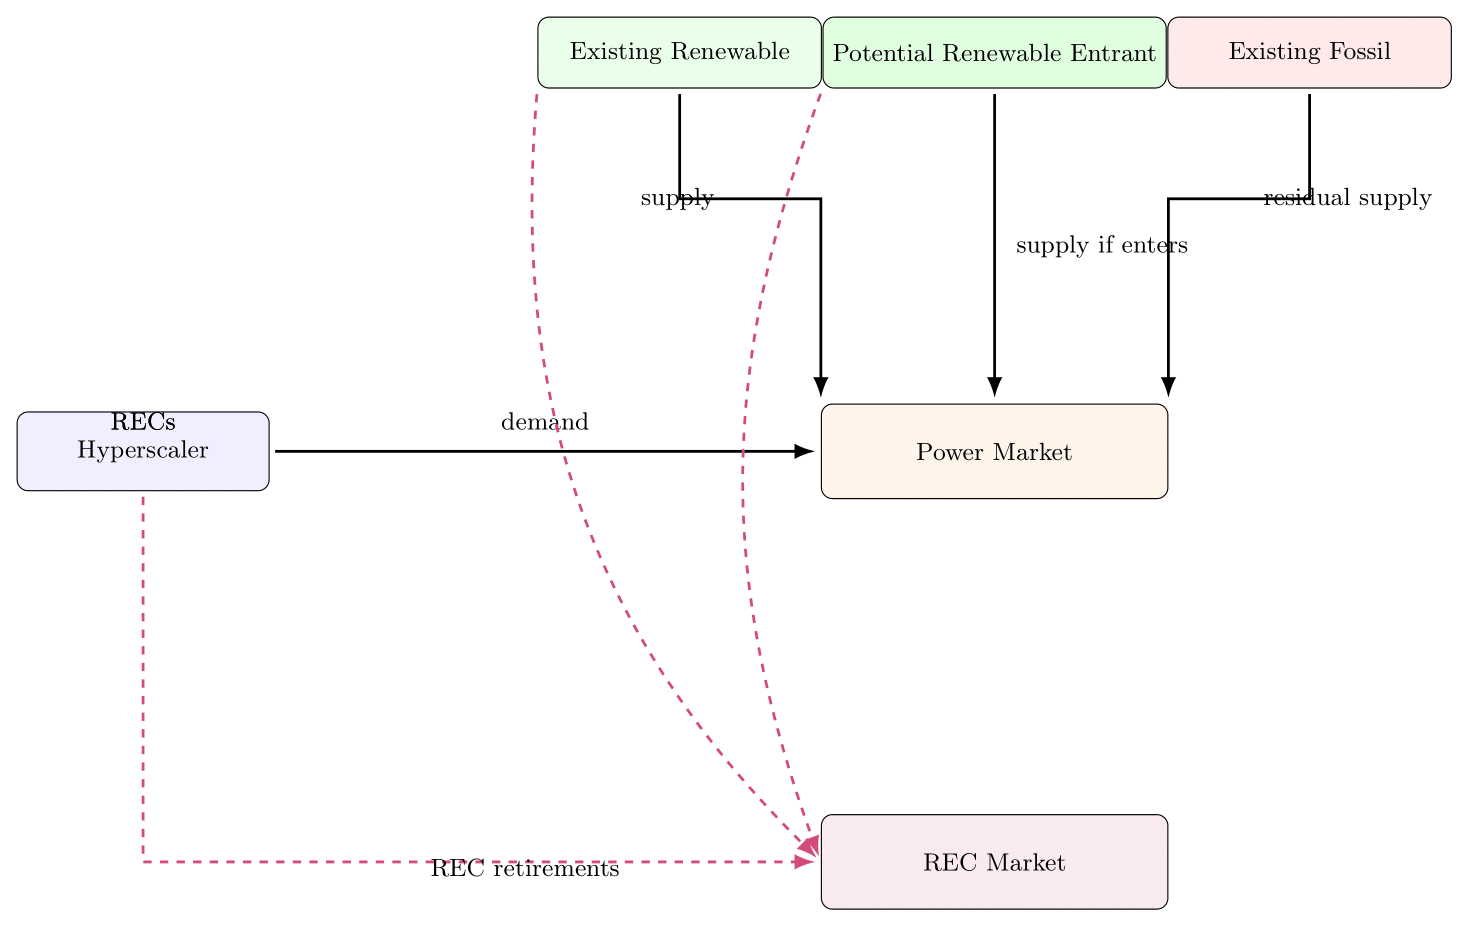
\includegraphics[width=0.5\linewidth]{Figures/Agents-1.png}
    \caption{Agents in Model}
    \label{fig:Agents}
\end{figure}
The hyperscaler has inelastic demand $D^M_t=1$ in each period, and there is no outside demand ($D^O_t=0$).
Variable costs and emissions:
\[
c_F>0,\quad e_F>0,\qquad c_{R_1}=c_{R_2}=0,\quad e_{R_1}=e_{R_2}=0.
\]
Capacities/output (deterministic to highlight timing):
\[
x_{R_1,1}=1,\ \ x_{R_1,2}=0;\qquad x_{R_2,1}=0,\ \ x_{R_2,2}\in\{0,1\};\qquad 
\]
\begin{center}
    $x_{F,t}\in\{0,1\}.$
\end{center}

Renewables are \emph{complementary in time}: $R_1$ only produces in $t=1$, while $R_2$ (if it enters) only produces in $t=2$.
The fossil unit can meet any residual demand.

\paragraph{Dispatch and prices.}
Competitive dispatch follows merit order. If a renewable is available in $t$, it clears the 1~MWh load at $p_t=0$; otherwise $F$ clears at $p_t=c_F$.
Hence, without $R_2$ entry:
\[
p_1=0,\qquad p_2=c_F,\qquad \text{MCI}_1=0,\ \text{MCI}_2=e_F.
\]
With $R_2$ entered, $p_2=0$ as well.

\paragraph{REC mechanics and the timing parameter.}
Each MWh of renewable generates one REC in its production period. Let $S_t$ be REC supply, so without entry $S_1=1$, $S_2=0$; with entry $S_2=1$.
The hyperscaler targets $100\%$ coverage ($\phi=1$) under REC procurement with granularity parameter $h\in[0,1]$:
$h=0$ (annual matching, no timing), $h=1$ (hourly matching).
Let $R^{G}_t$ be granular retirements and $R^{A}$ annual-bucket retirements. Feasibility:
\[
\underbrace{R^G_t \ge h D^M_t}_{\text{granular}},\qquad
\underbrace{R^{A} \ge (1-h)(D^M_1{+}D^M_2)}_{\text{annual}},\qquad
\]

\paragraph{Potential entrant $R_2$.}
If $R_2$ enters, it produces $x_{R_2,2}=1$ in $t=2$. It pays entry cost $I>0$ financed at $1+r(\sigma^2)$.
We compare three procurement environments (which map to different cash-flow risk for $R_2$):
\begin{enumerate}
\item \emph{REC/merchant (no contract).} $R_2$ sells energy at $p_2$ and its REC at $p^{REC}_2$.
\item \emph{PPA.} $R_2$ receives a fixed transfer $\bar p$ per MWh in $t=2$ (energy+REC bundled); residual merchant exposure is zero in this toy case.
\item \emph{Colocation.} $R_2$ is fully contracted on-site at transfer $\tilde p$ per MWh in $t=2$ (no market risk).
\end{enumerate}
We keep discounting trivial (two periods, take $\beta=1$) to focus on timing and entry.

\paragraph{Outcomes by procurement regime.}
\subsection{Full Model}

\paragraph{Agents and primitives.}
We study a market with a large data center hyperscaler (e.g.\ Microsoft) and a set of generators indexed by owner $k$ and technology $l \in \{R,F\}$ (renewable or fossil).\footnote{Index individual plants by $g$ when convenient; technology $l(g)\in\{R,F\}$.} 
The hyperscaler procures electricity to minimize expected total costs by choosing (i) a long-term power supply arrangement $i\in\mathcal I$ and (ii) an emergency backup option $j\in\mathcal J$.

\vspace{0.5em}
\noindent\textbf{Key objects.} 
\begin{itemize}
\item For each generator $g$: capacity $O^{\max}_g$, variable cost $c_g$, emissions rate $e_g$, and stochastic availability.
\item For the hyperscaler: load $\{D^M_t\}_{t=1}^2$, backup option $j\in\{\text{none},\text{diesel},\text{storage}\}$, and procurement $i\in\{\text{REC}, \text{PPA}, \text{Colocation}\}$.
\end{itemize}

\subsection{Timing}

\textbf{Stage 0a (commitment):} The hyperscaler commits to procurement $i\in\mathcal I$ and backup $j\in\mathcal J$ (contract terms public).

\textbf{Stage 0b (entry):} A set of potential generators of both types observes $(i,j)$ and decides whether to enter. Entry costs are sunk upon entry.

\textbf{Stages 1--2 (operations):} In each period $t=1,2$, shocks realize (demand, renewable availability). The energy market dispatches competitively; RECs are issued, banked, and retired subject to granularity rules (the ``timing wedge''). Agents discount with factor $\beta\in(0,1)$ across the two operating periods.

\subsection{Hyperscaler problem (commitment stage)}

The hyperscaler chooses $(i,j)$ to minimize expected total costs:
\begin{equation}
\label{eq:hyper_obj}
\pi_{\text{hyper}} \;=\; \min_{i\in\mathcal I,\, j\in\mathcal J}
\left[
C^{\mathrm{cap}}_i + C^{\mathrm{op}}_i
+ P_{ij}\,C^{\mathrm{out}} + \bar C^{\mathrm{env}}_{ij}
\right],
\end{equation}
where $P_{ij}=P_i P_j$ is the probability that both the contracted source fails and the backup is unavailable, $C^{\mathrm{out}}$ is the outage loss, and $\bar C^{\mathrm{env}}_{ij}=\mathbb{E}[f(\Delta E_{ij})\,C^{\mathrm{env}}_{ij}]$ is the expected reputational cost as a function of the emissions delta $\Delta E_{ij}\equiv E^{\text{with DC}}-E^{\text{without DC}}$.

\paragraph{Contract menu.}
\begin{itemize}
\item \emph{REC/merchant} ($i=\text{REC}$): the hyperscaler buys energy from the grid and retires RECs; generators remain merchant for energy and REC revenue.
\item \emph{PPA} ($i=\text{PPA}$): a renewable generator sells a fixed quantity $\bar q$ each period at price $\bar p$; residual is merchant.
\item \emph{Colocation} ($i=\text{Colo}$): a dedicated renewable unit (optionally with storage) physically colocated with the data center delivers $Q^{\text{colo}}_t$; residual met from the grid. Colocation fully insulates the generator from market risk.
\end{itemize}

\paragraph{Backup.} $j\in\{\text{none},\text{diesel},\text{storage}\}$ affects both reliability ($P_j$) and emissions: diesel has $e_j>0$, storage has $e_j=0$ if charged by colocated renewables.

\subsection{Entry (Stage 0b)}

Potential entrants of type $l\in\{R,F\}$ decide to enter before operations. Let $I_g$ be the sunk entry cost for plant $g$, and let $r(\sigma^2)$ be the project’s financing rate, strictly increasing in the variance of net operating cash flows $\sigma^2$ (a reduced-form cost-of-capital channel). For a renewable merchant entrant,
\begin{equation}
\label{eq:profit_merchant}
\Pi^{R,\text{merch}}_g \;=\; \mathbb{E}\!\left[\sum_{t=1}^{2}\beta^{t-1}\big((p_t+p^{REC}_t) x_{g,t}-c_g x_{g,t}\big) \right]
\;-
\end{equation}
\begin{center}
    $\; I_g\,\Big(1+r(\sigma^2_{\text{merch}})\Big).$
\end{center}
Under a PPA for $\bar q\le O^{\max}_g$ at price $\bar p$,
\begin{equation}
\label{eq:profit_ppa}
\Pi^{R,\text{ppa}}_g \;=\; \sum_{t=1}^{2}\beta^{t-1}\left[\bar p\,\bar q + (p_t+p^{REC}_t)(x_{g,t}-\bar q)_+ - c_g x_{g,t}\right]
\;-
\end{equation}
\begin{center}
    $\; I_g\,\Big(1+r(\sigma^2_{\text{ppa}})\Big).$
\end{center}
Under colocation (full revenue and REC certainty for the contracted amount),
\begin{equation}
\label{eq:profit_colo}
\Pi^{R,\text{colo}}_g \;=\; \sum_{t=1}^{2}\beta^{t-1}\left[\tilde p_t\, Q^{\text{colo}}_t - c_g x_{g,t}\right]
\;-\; I_g\,\Big(1+r(0)\Big),
\end{equation}
where $\tilde p_t$ is the contracted transfer for colocated output. For fossil $F$, replace $(p_t+p^{REC}_t)$ by $p_t$.

\paragraph{Free entry.} With a continuum of potential entrants and competitive supply of projects, free entry implies zero-profit conditions for marginal entrants of each type/contract:
\begin{equation}
\Pi^{l,\cdot}_g \;\le\; 0\quad\text{for all }g,\qquad
\Pi^{l,\cdot}_g=0\ \text{if }g\ \text{enters},\qquad l\in\{R,F\}.
\end{equation}
Because $r(\sigma^2)$ increases in variance and colocation eliminates variance,
\begin{equation}
r(0)\;\le\; r(\sigma^2_{\text{ppa}})\;\le\; r(\sigma^2_{\text{merch}}),
\quad\Rightarrow\quad
\text{entry}_{\text{colo}} \;\ge\;
\end{equation}

\begin{center}
    $\text{entry}_{\text{ppa}} \;\ge\; \text{entry}_{\text{merchant}}
\ \ \text{(all else equal).}$
\end{center}

\subsection{Operations subgame (two periods $t=1,2$)}

\paragraph{Demand.} Total load each period is $D_t=D^M_t+D^O_t$. Net grid draw by the hyperscaler is
\begin{equation}
\label{eq:grid_draw}
G^M_{t} \;=\; \big(D^M_t - Q^{\text{contract}}_{i,t} - Q^{\text{colo}}_t - B_{j,t}\big)_+,
\end{equation}
where $Q^{\text{contract}}_{i,t}$ is the (possibly firm) delivery under $i$ and $B_{j,t}$ is backup output.

\paragraph{Availability.} Each generator $g$ is either fully available or off:
\begin{equation}
x_{g,t}\in\{0,O_g^{\max}\},\quad \Pr(x_{g,t}=O_g^{\max})=\alpha_{g,t}.
\end{equation}

\paragraph{Energy dispatch and price.} Given the set of available units $\mathcal G_t$, the competitive dispatch solves
\begin{equation}
\label{eq:dispatch}
\min_{\{x_{g,t}\}} \ \sum_{g\in\mathcal G_t} c_g x_{g,t} \qquad
\text{s.t.}\quad 
\end{equation}
\begin{center}
    $\sum_{g\in\mathcal G_t} x_{g,t} + B_{j,t} + Q^{\text{colo}}_t \;=\; D_t,\ \ x_{g,t}\in\{0,O_g^{\max}\}.$
\end{center}
Let $\lambda_t$ be the energy balance multiplier. The locational marginal price (LMP) is $p_t=\lambda_t=c_{g^*(t)}$, where $g^*(t)$ is the marginal unit at the optimum.

\paragraph{REC issuance, banking, and the timing wedge.}
Renewables mint one REC per MWh:
\begin{equation}
r_{g,t}=\mathbf 1\{l(g)=R\}\,x_{g,t},\qquad S_t=\sum_g r_{g,t}.
\end{equation}
A stock of banked RECs evolves:
\begin{equation}
\label{eq:bank}
K_{t+1}=(1-\delta)K_t+S_t - R^{\text{ret}}_t,\qquad K_t\in[0,\bar K],\quad t=1,
\end{equation}
with terminal $K_3$ free (or bounded).

To formalize matching granularity, fix a parameter $h\in[0,1]$:
\(h=0\) is annual bucket matching; \(h=1\) is full hour/period matching.
Let $R^{M,G}_t$ be the hyperscaler's \emph{granular} retirements in period $t$
and $R^{M,A}$ its \emph{annual bucket} retirements.
The hyperscaler targets a renewable share $\phi\in[0,1]$ of its total consumption.
Feasibility and obligations:
\begin{align}

\label{eq:gran_req}
&\textbf{(Granular requirement)} 

& R^{M,G}_t \ge h\,\phi\,D^M_t,

&& R^{M,G}_t \ \le\ S^{\text{qual}}_t, \quad t=1,2,\\

\label{eq:annual_req}
&\textbf{(Annual requirement)} & 

R^{M,A} \ \ge\ (1-h)\,\phi\,(D^M_1+D^M_2), \\

&& R^{M,A} \ \le\ K_1+S_1+S_2 - (R^{M,G}_1+R^{M,G}_2),
\end{align}

where $S^{\text{qual}}_t\le S_t$ denotes RECs eligible by geography/tier.
The \emph{timing wedge} is the load not covered by same-period renewable matching:


\begin{equation}
\label{eq:wedge}
w_t(h) \;=\; G^M_t - R^{M,G}_t \ \ \ (\ge 0 \text{ if } h>0 \text{ binds}),
\qquad
\end{equation}

\begin{center}
    $ W(h)=\sum_{t=1}^2 \mathbb{E}[w_t(h)].$
\end{center}

\paragraph{REC market clearing and prices.}
Given banking \eqref{eq:bank} and obligations \eqref{eq:gran_req}--\eqref{eq:annual_req}, the competitive REC allocation minimizes present cost of compliance:
\begin{equation}
\begin{aligned}
\min_{\{R^{\text{ret}}_t,K_2,R^{M,G}_t,R^{M,A}\}} \quad 
& \sum_{t=1}^{2} \beta^{t-1} p^{REC}_t R^{\text{ret}}_t \;+\; \sum_{t=1}^{2} \beta^{t-1} \overline p^{\text{ACP}}_t\, \text{short}_t \\
\text{s.t.}\quad 
& \eqref{eq:bank},\ \eqref{eq:gran_req},\ \eqref{eq:annual_req},\quad
\end{aligned}
\end{equation}
\begin{center}
$R^{\text{ret}}_t = R^{M,G}_t + \mathbf 1\{t=2\}R^{M,A} + R^{\text{LSE}}_t - \text{short}_t,\\
& R^{\cdot}\ge 0,\ \text{short}_t\ge 0.$
\end{center}
Let $\mu$ be the annual-constraint multiplier and $\nu_t$ the granular multipliers.
Then the effective shadow value of a qualifying REC used in $t$ is
\begin{equation}
\label{eq:rec_shadow}
\tilde p^{REC}_t \;=\; p^{REC}_t \;+\; \nu_t \;+\; \mathbf 1\{t=2\}\,\mu.
\end{equation}
With interior banking, the Euler condition implies
\begin{equation}
\label{eq:rec_euler}
p^{REC}_1 \;=\; \beta(1-\delta)\, \mathbb E\left[p^{REC}_2\right],
\end{equation}
and $p^{REC}_t\le\overline p_t^{\text{ACP}}$ with equality if shortfalls occur.

\paragraph{Emissions and carbon intensity.}
Total emissions in $t$ are
\begin{equation}
E_t = \sum_{g\in\mathcal G_t} e_g x_{g,t} + e_j B_{j,t}.
\end{equation}
Define average and marginal carbon intensity:
\begin{equation}
\text{ACI}_t = \frac{E_t}{\sum_g x_{g,t}+B_{j,t}}, 
\qquad \text{MCI}_t = e_{g^*(t)}.
\end{equation}
Microsoft’s attributable marginal emissions under $(i,j)$:
\begin{equation}
\text{MME}_{i,j} \;=\; \sum_{t=1}^2 \beta^{t-1}\,\mathbb E\!\left[\text{MCI}_t \cdot G^M_{t}\right],
\end{equation}
with $G^M_t$ in \eqref{eq:grid_draw}.

\subsubsection{Equilibrium}

Given $(i,j)$ and the set of entrants from Stage 0b, a \emph{competitive two-period operating equilibrium} is a tuple 
\[
\big\{\{x_{g,t}\}, \{p_t\}, \{p^{REC}_t\}, K_2, \{R^{M,G}_t\}, R^{M,A}\big\}_{t=1,2}
\]
such that (i) dispatch \eqref{eq:dispatch} clears energy with $p_t=c_{g^*(t)}$; (ii) REC issuance/banking/retirements satisfy \eqref{eq:bank}, \eqref{eq:gran_req}--\eqref{eq:annual_req}, and REC prices satisfy \eqref{eq:rec_euler}; and (iii) backup and colocation quantities meet \eqref{eq:grid_draw}. A \emph{subgame-perfect equilibrium} of the full game consists of $(i^*,j^*)$ solving \eqref{eq:hyper_obj}, a set of entrants satisfying free-entry conditions, and a competitive operating equilibrium in each period.


\subsubsection{Mechanisms and Equilibrium Implications}

Three mechanisms drive outcomes. First, procurement choices shape operational emissions through the
\emph{timing wedge} between load and renewable generation. Colocation with storage shrinks this wedge by re-timing renewable energy into high-carbon hours; diesel backup increases emissions. 

Second, contract type alters financing risk: PPAs reduce $\sigma^2$ relative to RECs, and colocation eliminates it. Lower variance reduces $r(\sigma^2)$, encouraging renewable entry. 

Third, equilibrium carbon intensity reflects both the short-run operational effect and the long-run investment effect. 

\subsubsection{Implications}

Our model provides a set of empirical predictions about how hyperscalers’ procurement choices affect both costs and carbon intensity. On the demand side, as the spread between the cost of procuring electricity from renewable sources and from the open market widens, hyperscalers are more likely to turn to the open market and less likely to contract renewables. At the same time, as hyperscaler demand for electricity grows, the environmental cost of their consumption rises, and the benefits of carbon-free procurement mechanisms such as PPAs and colocation increase. These benefits scale with both the overall carbon intensity of grid electricity and the size of the hyperscaler’s load: the dirtier and larger the load, the greater the incentive to secure clean and reputationally valuable supply.

On the supply side, the model emphasizes that because renewable generation is intermittent, incremental data center demand tends to raise fossil generation unless there is sufficient storage to shift renewable energy across periods. The timing mismatch between hyperscaler load and renewable output—the “timing wedge”—is therefore central to understanding operational emissions outcomes. Colocation with storage can shrink this wedge by re-timing renewable production to high-carbon hours, while diesel backup increases emissions during outages.

These mechanics give rise to several testable implications. First, REC purchases on their own do not alter short-run carbon intensity, since they are purely financial transfers. Their effect arises only in the medium run, if REC demand raises REC prices and induces new renewable capacity to come online. PPAs without firming behave similarly in operational terms, but they reduce generators’ revenue risk and financing costs, which increases renewable entry relative to REC-only arrangements. Colocation has a more immediate impact: behind-the-meter renewable output reduces a hyperscaler’s net grid draw exactly when the colocated plant is producing, lowering local marginal emissions exposure. The effect is strongest when renewable output is correlated with hyperscaler load. Adding storage to colocation further enhances this benefit by shifting surplus renewable production to periods when demand is high and marginal carbon intensity is greatest, sharply reducing emissions attributable to the data center. This also can an emissions effect as the reduced timing wedge better matches power, and the behind-the-meter power can add resilience to the grid. By contrast, reliance on diesel backup increases operational emissions whenever it is deployed.

Finally, the model predicts an investment hierarchy driven by financing risk: colocation, by fully eliminating revenue variance, induces the largest increase in renewable entry, followed by PPAs, and then REC purchases. This creates a long-run ordering in expected carbon reductions. Moreover, because colocated renewables reduce grid purchases at the hyperscaler’s node, emissions fall locally, though congestion and flow adjustments may increase carbon intensity in neighboring nodes unless total renewable capacity expands.

Together, these predictions imply that (i) REC purchases yield little immediate emissions reduction but may encourage new renewable entry; (ii) PPAs accelerate renewable deployment by reducing financing risk, though without firming they do not improve operational carbon intensity in the short run; and (iii) colocation—especially when paired with storage—directly lowers hyperscaler-attributable emissions by addressing the timing wedge between renewable generation and hyperscaler demand.

\section{Empirical Overview}\label{Sec::Methods}

We estimate the causal effect of AI workloads on four outcomes in wholesale electricity markets: local power quality, fossil fuel demand, wholesale prices, and the differential response across training versus inference phases. The central identification problem is that the objects of interest such as the timing, location, and intensity of compute activity at individual data centers, are proprietary. We observe neither training start dates nor facility-level load; instead, we observe publicly announced model release dates, the geographic footprint of hyperscaler data centers, and zonal market outcomes. Our strategy exploits model releases as the observable shock and uses difference-in-differences to recover treatment effects from the remaining variation.

\subsection{Identification}\label{EconometricModel}

Let $Y_{it}$ denote an outcome (power quality, fossil generation, or price) for zone $i$ in period $t$, and let model release $m$ occur at date $r_m$. Zones linked to the releasing firm's data center footprint constitute the treated group for event $m$; zones without exposure to that firm's AI activity in the event window form the control group. Under the standard parallel-trends and no-anticipation assumptions, differencing outcomes across treated and control zones before and after $r_m$ identifies the average treatment effect on the treated. Because our outcomes, wholesale prices, fossil generation, voltage distortion, are transmitted through markets and the physical grid rather than through proprietary firm-level data, this approach follows a long tradition of recovering unobservable inputs from observable market equilibria \citep{fowlie2012industrial, card1994minimum, greenstone2014environmental}.

Four features of our setting complicate a textbook two-period DiD. First, training windows are unobserved: we know when a model was released but not when its training began, so the ``treatment date'' is imprecise. Second, releases are staggered across firms and calendar time, which under treatment-effect heterogeneity causes two-way fixed effects estimators to weight already-treated units as implicit controls for later-treated units \citep{goodman2021difference, sun2021treatment, callaway2021difference, borusyak2024revisiting}. Third, parallel trends is not innocuous in electricity markets, where fuel prices, weather, and secular load growth move outcomes in ways potentially correlated with data center siting. Fourth, treatment exposure itself must be constructed: no dataset directly links model releases to zonal load, and assigning generators and facilities to market zones requires substantial preprocessing (see Appendix \ref{zonalMappingEfforts}).

We address the first two issues with a stacked event-study design that anchors treatment on observed release dates and builds clean control groups for each release cohort, developed in Section \ref{subsec:eventstudy}. We address the third through pre-trend tests, placebo exercises, and controls for fuel costs, temperature, and renewable output (Section \ref{Robustness}). The fourth is resolved in our data construction, described in Section \ref{sectionData}.

\section{Estimation Strategy}\label{sec:empirical}

To address the inexact information about training windows and release times, we estimate dynamic treatment effects at multiple horizons relative to model release dates. This approach, referred to as an event study or \textbf{stacked difference-in-differences} in econometrics, offers three advantages over the standard pre/post comparison discussed earlier: (1) it does not require observing the true training start date, instead using release timing as the anchor; (2) it also provides a direct test of the parallel trends assumption through examination of pre-release coefficients; and (3) it allows the data to reveal the temporal profile of effects rather than imposing an arbitrary discontinuous treatment structure.

\subsection{Stacked DiD with Multiple Horizons}%Event-Study Framework}
\label{subsec:eventstudy}
Formally, we define treatment exposure relative to each model's release date $r_m$ for both training and release: \textbf{1) Training windows:} The period $[r_m - \bar{\tau}_{\text{train}}, r_m)$ preceding release, during which computational resources are devoted to model training. We remain agnostic about the exact training start date; our identifying assumption is that training activity is elevated in the months before release and that any pre-existing differential trends would manifest in the earlier leads. \textbf{2) Inference window:} The period $[r_m, r_m + \bar{\tau}_{\text{infer}}]$ following release, during which the model is deployed for inference via API access or public availability.


\subsubsection{Stacked Difference-in-Difference}

Model releases occur at different calendar dates, creating a staggered adoption setting. Recent econometric literature has demonstrated that conventional two-way fixed effects (TWFE) estimators as is the case in the estimates from traditional difference-in-differences. 
can produce biased estimates under treatment effect heterogeneity 
\cite{goodman2021difference, sun2021treatment, callaway2021difference, borusyak2024revisiting}. Treatment effect heterogeneity means the policy works differently for different places or periods, which can distort standard difference-in-differences estimates. The bias arises because TWFE implicitly uses already-treated units as controls for later-treated units, and differences in treatment effects across cohorts or over time contaminate the estimated average effect. 

In our setting, consider regions as units and AI model releases as treatments inducing increased data center power demand. A ``cohort" comprises regions whose data centers began significant AI workloads at the same time. Suppose Region A adopted AI workloads in 2022 while Region B adopted in 2023. When estimating treatment effects for Region B, TWFE implicitly uses Region A as a control—but Region A in 2023 is not untreated; its data centers have been running AI workloads for a year. If treatment effects evolve over time (e.g., power demand grows as AI infrastructure scales), comparing Region B's outcomes against Region A's already-treated outcomes introduces bias. Staggered design provides heterogeneity-robust estimators that solve for this exact issue.

%\nb{Can you explain the previous sentence in terms of data centers and time wrt power demand? It is hard to know what already-treated, later-treated units, cohorts etc mean.}

To address this, we use a stacked DiD model~\cite{cengiz2019effect, deshpande2019screened}, where we construct a stacked dataset where each model release defines a separate ``sub-experiment.'' The idea here is to construct, for each treatment cohort, a separate sub-experiment using only units that are genuinely untreated at the time of that cohort's adoption. By stacking these sub-experiments—each with its own clean control group of not-yet-treated regions—we ensure that no already-treated unit ever serves as a control, thereby eliminating the bias that arises when treatment effects are heterogeneous across cohorts or time.

Formally, for each release event $m$, we create a dataset containing: (i) Treated units -- Regions linked to the releasing company's AI data centers. (ii) Control units -- Regions with no AI data center exposure during the event window, or regions whose treatment occurs sufficiently far from event $m$ that they serve as clean controls.
\begin{itemize}
    \item Time window: A symmetric window around $r_m$, e.g., $[r_m - K, r_m + K]$ for some horizon $K$.
\end{itemize}

Following \cite{wing2024stacked}, we then stack these sub-experiments and estimate:
\begin{equation}
Y_{i,t,m} = \sum_{k=-K}^{K} \beta_k \cdot D_{ut}^k  + \delta_t + \mathbf{X}_{ut}'\theta + \varepsilon_{ut}
\label{eq:stacked}
\end{equation}
where $\gamma_{u}$ are unit-by-event fixed effects, $\delta_{u}$ are time-by-event fixed effects, $\mathbf{X}_{ut}'\theta$ represents controls, and the coefficients $\{\beta_k\}$ trace out the dynamic treatment effect at each event-time horizon $k$. Standard errors are clustered at the unit level to account for correlation across events within the same region.


\subsection{Estimating Power Quality}

Our power quality analysis estimates the following stacked DiD specification at the utility-month level:
\begin{equation}
\text{PowerQuality}_{ut} = \sum_{k=-K}^{K} \beta_k^{PQ} \cdot D_{ut}^k + \gamma_u + \delta_t + \mathbf{X}_{ut}'\theta + \varepsilon_{ut}
\label{eq:pq_eventstudy}
\end{equation}
where:
\begin{itemize}
    \item $\text{PowerQuality}_{ut}$ is the Whisker Labs Consumer Power Quality Index for utility $u$ in month $t$;
    \item $D_{ut}^k = \mathbf{1}[\text{event-time} = k] \times \text{Treated}_u$ indicates that utility $u$ is $k$ periods from the release date of a model linked to an AI data center in its service territory;
    \item $\gamma_u$ are utility fixed effects absorbing time-invariant characteristics;
    \item $\delta_t$ are calendar month fixed effects absorbing common temporal shocks;
    \item $\mathbf{X}_{ut}$ includes time-varying controls (weather, regional load).
\end{itemize}

We estimate an analogous specification for total harmonic distortion (THD):
\begin{equation}
\text{THD}_{ut} = \sum_{k=-K}^{K} \beta_k^{THD} \cdot D_{ut}^k + \gamma_u + \delta_t + \mathbf{X}_{ut}'\theta + \varepsilon_{ut}
\label{eq:thd_eventstudy}
\end{equation}

% \paragraph{Identifying Assumption.} \nb{Arent we moving this to 3.5 or 3.6?} The key identifying assumption is that, absent the AI model release, treated and control utilities would have followed parallel trends in power quality. We assess this assumption by examining the estimated coefficients $\{\beta_k : k < 0\}$ in the pre-release period. Under parallel trends, these coefficients should be statistically indistinguishable from zero. Systematic pre-trends would indicate either (a) anticipatory effects, (b) confounding from correlated unobservables, or (c) differential trends predating treatment.

\subsection{Estimating Fossil Fuel Demand}

Power demand analysis proceeds at the generator-month level, exploiting finer geographic resolution. We maintain the stacked DiD structure while incorporating instrumental variables to address the price endogeneity concern:

\paragraph{First Stage.} We instrument for electricity prices using supply-side cost shifters:
\begin{equation}
p_{it} = \pi_0 + \pi_1 \text{HeatRate}_{it} + \pi_2 \text{GasPrice}_{t} + \gamma_i + \delta_t + \mathbf{X}_{it}'\pi_3 + \nu_{it}
\label{eq:firststage}
\end{equation}
where $\text{HeatRate}_{it}$ captures the thermal efficiency of generator $i$ and $\text{GasPrice}_t$ is the contemporaneous natural gas spot price. These instruments satisfy relevance (they are primary determinants of marginal generation costs) and exclusion (they affect demand only through their impact on prices, not through direct effects on AI workload scheduling or other consumption decisions).

\paragraph{Second Stage.} We estimate the stacked DiD specification using predicted prices:
\begin{equation}
\text{FossilDemand}_{it} = \sum_{k=-K}^{K} \beta_k^{FD} \cdot D_{it}^k + \eta \hat{p}_{it} + \gamma_i + \delta_t + \mathbf{X}_{it}'\theta + \varepsilon_{it}
\label{eq:demand_eventstudy}
\end{equation}
where $D_{it}^k$ indicates event-time relative to model releases linked to AI data centers in generator $i$'s service area.

The coefficients $\{\beta_k^{FD}\}$ capture the dynamic effect of AI activity on fossil fuel demand. Negative values of $k$ (pre-release) correspond to the training phase; positive values correspond to inference. The price coefficient $\eta$ controls for supply-driven price movements and provides a scaling factor for welfare calculations. Difference between samples in our main analyses are highlighted in the Appendix in Subsection \ref{subsec:differences}.

%\niranjan{Mention how the data is used to learn/estimate the co-efficients.}
%\niranjan{Add an equation here and refer to it in the text above.}

% \end{figure}
% \subsection{Empirical Strategy Details}
% This section presents our identification strategy for estimating the causal effects of AI model development on electricity grid outcomes. We analyze two primary outcomes: (1) power quality degradation at the utility level, and (2) fossil fuel generation demand at the generator level. Our approach employs an event-study framework centered on AI model release dates, with distinct treatment windows corresponding to the training and inference phases of AI development. We address identification challenges arising from staggered treatment timing, data limitations in linking models to specific training locations, and potential violations of parallel trends.



\subsection{Estimating Price Effects}\label{PriceEffects}
% \nb{Make this more explanatory for someone who knows almost nothing about supply/demand and their relationships.}
Beyond quantity effects, we estimate how AI-driven demand increases affect electricity prices. The key economic insight is that price impacts depend on supply flexibility: when generators can easily expand output, demand increases are absorbed with minimal price changes, but when supply is constrained, demand shocks translate primarily into higher prices. The supply elasticity $\varepsilon^s$—the percentage change in quantity supplied per one percent price change—quantifies this responsiveness.

Our estimation proceeds in two steps. First, we use our IV estimates to quantify how AI activity shifts demand:
\begin{equation}
\Delta \widehat{\text{FossilDemand}}{it} = \hat{\beta} \cdot \Delta \text{AI}{it}
\label{eq:demand-change}
\end{equation}

Second, we trace this shift through the supply curve. With linear supply $Q^s=a+b\cdot p_i$, the price change is $\Delta p=\hat{\beta}\cdot \frac{\Delta AI_{it}}{b}$, or in elasticity form:

\begin{equation}
\% \Delta p = \frac{\% \Delta Q^d}{\varepsilon^s}
\label{eq:price-impact-elasticity}
\end{equation}

We estimate $\varepsilon^s$ via IV regression of quantity on price in log-log form, using demand-side instruments (weather-driven load variation and industrial production indices).

We focus on PJM at the zonal level for this analysis. We restrict to a single ISO because differing market structures make prices incomparable across ISOs, and choose PJM because it is the largest (65 million people, 13 states), includes key data center states (Virginia, Pennsylvania), and provides 20 diverse pricing zones. Because observed training locations are outside PJM, this analysis uses the broader model set only.
% \paragraph{Demand Change from Treatment Effect.} The estimated coefficient $\hat{\beta}$ gives the predicted demand change for a given change in AI activity:
% \begin{equation}
% \Delta \widehat{\text{FossilDemand}}_{it} = \hat{\beta} \cdot \Delta \text{AI}_{it}
% \label{eq:demand-change}
% \end{equation}

% \paragraph{Price Impact via Supply Elasticity.} A demand shift $\Delta Q^d$ yields a price change determined by supply responsiveness. With linear supply $Q^s = a + b \cdot p$:
% \begin{equation}
% \Delta p = \frac{\hat{\beta} \cdot \Delta \text{AI}_{it}}{b}
% \label{eq:price-impact}
% \end{equation}
% In elasticity form, for a percentage demand increase $\% \Delta Q^d$:
% \begin{equation}
% \% \Delta p = \frac{\% \Delta Q^d}{\varepsilon^s}
% \label{eq:price-impact-elasticity}
% \end{equation}
% We estimate $\varepsilon^s$ via two-stage IV regression of quantity on price in log-log form, using demand-side instruments (weather-driven load variation and industrial production indices) rather than supply-side instruments. We then combine this elasticity estimate with the demand shift from earlier regressions to calculate price impact. For specifically this regression, we focus on the Independent System Operator (ISO) PJM at a zonal level. We choose to focus on one ISO because differently structured capacity markets and differing market structures mean that prices are not truly equivalent across ISOs. We focus specifically on PJM because it is the largest ISO by population including 65 million people over 13 states and crucially includes Virginia and Pennsylvania, two of the main data center hotbeds. PJM also has 20 diverse zones providing the neccecary granularity. Because the observed training locations are not in PJM, this analysis can only be conducted with the broader model set and not our conservative main analysis.
% \begin{center}
% \textit{[PLACEHOLDER: Table of models with verified training start dates, training end dates, and API/inference release dates from public announcements, papers, or regulatory filings]}
% \end{center}

\section{Validating Assumptions and Robustness}
\label{subsec:robustness}

We implement several diagnostic and robustness exercises to assess the credibility of our estimates.

\subsubsection{Sample Selection}

Our empirical strategy balances internal validity with external relevance. Our main sample comprises four models for which we observe exact training and inference dates as well as training location, and we employ propensity score matching (described in the appendix) to support the parallel trends assumption. We then report results for progressively larger samples of models and data centers, accepting weaker identification in exchange for broader coverage. This approach enables precise, well-identified estimates from our core sample while exploring heterogeneity and counterfactuals in extended samples, with appropriate caveats regarding the latter.

% We vary our sample, so we can provide highly robust estimates of treatment effects using a sample we have exceptional information about while exploring observed heterogeneity in larger samples to enable interesting analysis and counterfactual. We demonstrate robustness for the samples that are less controlled. In our main sample, we focus on four models for which we know exact training and inference dates as well as the location of training. We also utilize propensity score matching as described in the appendix in order to ensure the satisfaction of the parallel trends assumption. We report results for alternative progressively larger samples of models and datacenter with fewer robustness protections to provide a fuller picture with the caveat that less confidence exists in the estimated results. We feel that this conservative approach both allows us to make specific and measured statements and also broader but more impactful statements.

\subsubsection{Pre-Trends and Parallel Trends Testing}

Our primary test of the identifying assumption examines whether pre-release coefficients $\{\beta_k : k < 0\}$ are jointly indistinguishable from zero. We report:
\begin{itemize}
    \item Point estimates and confidence intervals for each lead coefficient.
    \item An F-test of the joint null hypothesis $H_0: \beta_{-K} = \beta_{-K+1} = \cdots = \beta_{-1} = 0$.
\end{itemize}
Significant pre-trends would undermine the causal interpretation of post-release estimates.

\subsubsection{Placebo Tests with Randomized Treatment Assignment}

To verify that our estimates reflect genuine treatment effects rather than spurious correlations or specification artifacts, we conduct placebo tests with randomly assigned treatment:
\begin{enumerate}
    \item \textbf{Random treatment timing:} We hold the set of treated units fixed but randomly reassign release dates drawn from the empirical distribution of actual release dates. Under the null of no effect, placebo estimates should center on zero.
    \item \textbf{Random treatment assignment:} We hold release timing fixed but randomly reassign treatment status across units. This tests whether results are driven by the specific geographic pattern of AI data center locations.
\end{enumerate}
% For each placebo design, we generate five draws and compare our actual estimates to the distribution of placebo estimates. We report the share of placebo estimates exceeding our point estimate in absolute value (a randomization inference p-value).

% \nb{Dana, add some text that says how this relates to the paragraph above?}
\subsubsection{Callaway-Sant'Anna Estimator}
% \paragraph{.} \nb{Can we move the robustness checks etc to 3.6?} 
%\nb{This requires some glue text to explain what issue this is addressing}

As a robustness check and to provide transparent decomposition of treatment effect heterogeneity, we also implement the \citet{callaway2021difference} estimator. Like the stacked approach, CS avoids using already-treated units as controls; however, rather than achieving this through sample construction, it does so by estimating separate ATT(g,t) parameters for each cohort g and time period t, then aggregating these to form summary measures. This approach explicitly avoids problematic comparisons and provides a framework for testing parallel trends through examination of pre-treatment ATT(g,t) estimates. 
\subsubsection{Time-Series Anomaly Detection}

As an internal consistency check, we apply time-series anomaly detection methods to the outcome variables in treated units. If AI model releases causally affect grid outcomes, we should observe detected anomalies clustering around treatment dates. Specifically:
\begin{enumerate}
    \item For each treated unit, we fit a baseline time-series seasonal ARIMA model to the pre-treatment period.
    \item We generate one-step-ahead forecasts and prediction intervals for the post-treatment period.
    \item We flag observations where realized values fall outside the 20\% prediction interval as anomalies.
    \item We test whether anomaly frequency is elevated in the post-treatment window relative to the pre-treatment window and relative to control units.
\end{enumerate}
This approach provides model-free evidence of structural breaks coinciding with treatment timing.

\subsubsection{Sensitivity to Treatment Definition}

Given uncertainty in linking models to specific training locations, we assess robustness to alternative treatment definitions in our less conservative analysis version:
\begin{enumerate}
    \item \textbf{Intensive margin:} Weight treatment by the number or capacity of AI data centers in the region, rather than using a binary indicator.
    \item \textbf{Dropping ambiguous cases:} Exclude model releases where the company operates data centers in multiple balancing authorities, restricting to cases with cleaner geographic attribution.
    \item \textbf{Verified timing subset:} Estimate separately on the subset of models with externally verified training windows.
    \item \textbf{Geographic Resolution and Robustness.} The generator-level data permit more granular treatment definitions than the utility-level power quality data. We exploit this flexibility by estimating specifications under alternative treatment definitions in terms of radius.
\end{enumerate}

\subsubsection{Heterogeneity by Model Characteristics}

We examine whether treatment effects vary with observable model characteristics:
\begin{itemize}
    \item Model scale (parameter count, reported compute).
    \item Company (to assess whether effects are driven by specific firms).
    \item Release year (to assess whether effects are changing over time).
\end{itemize}
Heterogeneity analysis both informs mechanisms and serves as a specification check: if effects are concentrated among larger models or models from companies with substantial AI infrastructure, this lends credibility to the AI-driven interpretation.
\subsection{Counterfactual Analysis}\label{counterfactuals}%Efficiency Impact Model}\niranjan{Compress}

We conduct three primary sets of counterfactual exercises to investigate how alternative evolutionary paths for AI compute might affect grid-level outcomes. Additional counterfactuals with results are highlighted in Appendix Subsection \ref{Appendix:Counterfactuals}.

\textbf{Model Scaling.} First, we examine the grid implications of continued growth in AI model size. Using the Epoch database to characterize trends in model parameters, we provide descriptive analysis of how increasing model scale translates into grid-level impacts. We then relate our estimated power demand coefficients to our power quality coefficients, enabling analysis of how changes in training and inference energy efficiency propagate to power quality outcomes.

\textbf{Geographic Redistribution.} Second, we leverage the geographic locations of data centers in conjunction with our econometric estimates to conduct counterfactuals focused on spatial reallocation of AI compute. We consider two scenarios. In the first, we simulate a shift from cloud-based to edge-based inference—reallocating inference demand from concentrated hyperscaler facilities to smaller data centers distributed closer to population centers. We implement this by redistributing our estimated inference demand impacts across data centers not currently classified as AI-focused. In the second scenario, we simulate relocating training workloads from population-dense regions on the East Coast to energy-abundant regions in the center of the country. For both geographic counterfactuals, we provide sensitivity analyses in the appendix to account for potential increases in communication costs and efficiency losses.

\textbf{Colocated on-site Power Generation.} Finally, we exploit a new feature in the Aterio data, namely a flag on data centers with on-site power generation. We re-estimate both our main models separately for generators with and generators without onsite power generation. We then report the impacts to power demand and power quality of either removing all onsite generation or having onsite generation for all data centers.


Together, these counterfactuals illuminate both how the grid might be affected by different trajectories for AI compute and which levers—geographic placement, workload composition, efficiency improvements—may be available to computer scientists and policymakers seeking to mitigate grid impacts.
%\niranjan{The main idea is to design regressors that can tell us how changes in efficiency e.g., reduction in model parameters, impacts power quality and demand. Note we already have a model for how the power quality changes for a certain set of AI model releases. We can use this to .... To do this we need... }

%Our methodology combines econometric estimates with data from the Epoch database on the number of parameters of models as well as estimates of the impacts of increasing model parameters on relative energy usage. We perform regressions on our coefficients on training compute FLOPS and parameters. This allows us to determine how relative increases in the model's efficiency can lead to changes in model power demand and quality.

%We also perform a techno-economic analysis of the impacts of increasing model size and the number of simultaneous GPUs on energy consumption. This analysis combines econometric estimates with experimental evidence we generated by training a subset of smaller models under different GPU counts and sizes, allowing us to directly observe the contribution of message passing between GPUs to total training energy costs. We essentially extrapolate our experimental results to larger production-level models to estimate the real-world impact of the power reductions from the experiments. Together, these approaches provide a framework for translating trends in AI model scaling into counterfactual grid-level impacts.

% We also run a difference-in-difference regression of the entire length of the interconnection queue and the length of the interconnection queue specifically for natural gas for counties before and after the announcement of a major data center.

% \begin{equation*}
% \text{TotalQueue}_{ct} = \alpha' 
% + \beta' \left( \text{Post}_{t} \times \text{Treatment}_{c} \right)
% + \gamma'_c + \delta'_t + \varepsilon'_{ct}
% \end{equation*}

% \begin{equation*}
% \text{GasQueue}_{ct} = \alpha 
% + \beta \left( \text{Post}_{t} \times \text{Treatment}_{c} \right)
% + \gamma_c + \delta_t + \varepsilon_{ct}
% \end{equation*}

% We also interact the capacity and square footage of the data center with the variable for after the data center's implementation to determine the impact of a MW of capacity from data centers on the interconnection queue. This provides an understanding of how natural gas investments increase following data center announcements and provides evidence for how data centers impact capacity investments.

% \begin{equation*}
%     \text{GasQueue}_{ct} = \alpha + \beta_1 \left( \text{Post}_{t} \times \text{Capacity}_{c} \right)+ \gamma_c + \delta_t + \varepsilon_{ct}
% \end{equation*}

% \begin{equation*}
%     \text{GasQueue}_{ct} = \alpha + \beta_2 \left( \text{Post}_{t} \times \text{SqFt}_{c} \right)+ \gamma_c + \delta_t + \varepsilon_{ct}
% \end{equation*}

% In order to consider the impacts of PPAs by data centers, we look at EIA form 860 data on capacity investments in counties with data centers as well as counties with PPAs by tech companies. PPA data comes from S\& P Capital IQ Pro and is used to perform difference-in-differences regressions of entry capacity of renewable resources on power purchase agreements. We further perform a similar regression of capacity investments in natural gas on announcements of data centers to determine whether PPAs are leading to more renewable or fossil fuel capacity additions.

% % 1. Renewable capacity entry and PPAs
% \begin{equation}
% \text{RenewCap}_{ct} 
% = \alpha 
% + \beta \, (\text{PPA}_c \times \text{Post}_t) 
% + \gamma_c + \delta_t 
% + \varepsilon_{ct}
% \end{equation}

% % 2. Fossil (natural gas) capacity entry and data center announcements
% \begin{equation}
% \text{GasCap}_{ct} 
% = \alpha 
% + \theta \, (\text{DCAnnounce}_c \times \text{Post}_t) 
% + \gamma_c + \delta_t 
% + \varepsilon_{ct}
% \end{equation}

% \subsection{Controls}
% \aruna{Not clear if we need this section given we discuss the controls in each of the specific section, thoughts?}
% The difference-in-differences framework relies on the assumption that, absent treatment, outcomes for treated and control groups would have evolved along parallel trends. Potential threats to this assumption include \emph{group-specific shocks} such as local infrastructure upgrades or outages that disproportionately affect power quality, \emph{anticipation effects} including preemptive grid adjustments ahead of a model release, and \emph{spillovers} like load shifting from nearby control regions. Any of these could bias estimated treatment effects if not properly accounted for. To mitigate these risks, we incorporate controls for weather and fuel prices, as well as geographic and temporal fixed effects. For instance, we explicitly model the impacts of weather conditions by including weather control variables to ensure that systematic climatic variation—which could influence both electricity demand and grid stability—does not confound our estimates.


\section{Data}\label{sectionData}
%\niranjan{To address the three questions we need the following data -- refer to data about variables of interest, control data}
%\niranjan{What we have now is the data of this kind. Who publishes it ... We combine these sources to obtain this data.}
Table \ref{tab:DataSources} summarizes the datasets we use to address each of our three research questions, distinguishing between variables of interest and the control variables described above. For variables of interest, we rely on \textbf{Aterio}, which provides comprehensive information on the location and history of data centers. The Aterio dataset documents when and where centers have been established, expanded, or retired, along with details on ownership and operational capacity (in MW). This allows us to identify data centers owned by specific hyperscalers and to quantify their scale over time. We then combine these data with external sources that provide the necessary controls.
\begin{table}[htbp]
\scriptsize % smaller font for compression
\centering
\caption{Data sources for each analysis question.}
\label{tab:DataSources}
\begin{threeparttable}
\begin{tabularx}{\linewidth}{lXXl}
\toprule
\textbf{Source} & \textbf{Content} & \textbf{Use in Analysis} & \textbf{\# Instances} \\
\midrule
\multicolumn{4}{c}{\textbf{Q1: Difference-in-Differences (Power Quality)}} \\
\midrule
Aterio & Data center locations, history, ownership, capacity (MW) & Define treatment regions; link AI model releases & 3862 data centers\\
Whisker Labs & CPQI (consumer reliability); THD (waveform distortion) & Outcome variables for DiD regressions & 2684 utility-months\\
EIA & Retail service territory maps & Define treatment/control boundaries & 72 utilities\\
\midrule
\multicolumn{4}{c}{\textbf{Q2: Instrumental Variables (Fossil Demand)}} \\
\midrule
EPA CAMPD & Hourly generator demand; heat rates & Fossil demand outcome; heat rate as instrument & 22 million generator-hours\\
S\&P Capital IQ & Natural gas prices & Instrument and fuel-cost control &12 Million location-day prices \\
Aterio & Data center proximity to generators & Treatment near releasing-company centers & 3862 data centers\\
Meteostat & Temperature, precipitation & Demand and renewable controls & 22 million location-hours\\
ISOs & Zonal wholesale prices & Market controls & 54 zones\\
\midrule
\multicolumn{4}{c}{\textbf{Q3: Counterfactual Analyses (Scaling \& Efficiency)}} \\
\midrule
Whisker Labs & CPQI; THD & Baseline power quality impacts for scaling projections & \\
Epoch & Model parameters, FLOPs, release dates & Scaling regressions; efficiency counterfactuals & 75 models\\
% GPU Experiments & Energy use with varying GPU counts/sizes & Extrapolate to production models & \\
\bottomrule
\end{tabularx}
\end{threeparttable}
\end{table}


%\niranjan{This following paragraph can be compressed since we detail the sources under 5.2 anyway. Just keep the first line and toss the rest. If there are additional pieces of information here then merge them into 5.1 and 5.2 as appropriate.}
 %Weather data come from \textbf{Meteostat}, which reports hourly temperature and precipitation; fuel cost data are obtained from \textbf{S\&P Capital IQ Global}, which publishes historical natural gas price series; and generator-level demand and heat rate data are published by the \textbf{EPA} through the Continuous Air Monitoring and Power Data (CAMPD). In addition, we construct zonal market boundaries using maps provided by \textbf{U.S. Independent System Operators (ISOs)} and merge these with ISO wholesale price data. Finally, we use geographic service territory files from the \textbf{EIA} to ensure consistent alignment of generator-, zonal-, and retail-level observations across datasets.  
\subsection{Variables of Interest}
%\niranjan{separately specify the variables of interest and the data needed for each question here. call them out explicitly with bold face or italics or some headings.}

We use four primary datasets for our outcomes of interest. First, the \textbf{Consumer Power Quality Index (CPQI)} from \cite{WhiskerLabs_THD_2024} provides a composite measure of consumer-facing reliability events (surges, sags, brownouts, interruptions), summarizing frequency and severity of power deviations at the household level. Second, \textbf{Total Harmonic Distortion (THD)} data from \cite{WhiskerLabs_THD_2024} offers a \emph{technical measure of waveform distortion}, quantifying voltage deviation from a clean 60-Hz sine wave. Elevated THD indicates grid stress, reduces motor efficiency, and shortens equipment lifespan. Figure \ref{fig:THD} illustrates how harmonics alter voltage sine waves, reducing power reliability. Since THD data are more recent than CPQI, fewer model releases are available for THD analysis. Third, we incorporate \textbf{generator demand} from EPA's CAMPD database, providing \emph{hourly plant-level demand} that captures local operating characteristics. CAMPD data span 2021--2023, constraining analysis to AI model releases within that period. Finally, we combine \textbf{wholesale zonal price} data provided by Independent System Operators (ISOs) to determine AI impacts on price.
\subsection{Control Variables}

For the \textbf{power quality regressions}, we use a parsimonious specification with only time and geographic fixed effects, which absorb seasonal patterns, long-run trends, and location-specific differences, allowing us to test whether data center activity coincides with reliability declines beyond geography and time. In contrast, the \textbf{generator demand regressions} employ a richer set of controls to address endogeneity, using \emph{generator heat rates} from EPA CAMPD and \emph{natural gas prices} from S\&P Capital IQ Global as instruments in a two-stage least squares framework, along with CAMPD’s hourly generator demand data (2021–2024). We also incorporate \emph{Meteostat} weather variables (temperature, dewpoint, precipitation) to capture demand and renewable variability, and \emph{ISO} market data based on boundary maps to ensure spatial consistency. Finally, \emph{EIA retail service territory files} reconcile generator-, zonal-, and retail-level observations into a consistent framework.


% For the \textbf{power quality regressions}, we deliberately keep controls parsimonious. Because the areas for which power quality is measured are much larger and the available dataset is significantly smaller, we restrict the specification to time and geographic fixed effects. These absorb broad seasonal patterns, long-run trends, and location-specific differences that could confound observed changes in power quality. We do not include fuel or generator-level variables here, because the goal is to isolate whether data center activity coincides with localized deteriorations in reliability beyond what is explained by geography and time.  


% In contrast, for the \textbf{generator demand regressions}, we employ a richer set of external data sources to address the endogeneity of prices and generation. In particular, we use \emph{generator heat rates} from the EPA’s Continuous Air Monitoring and Power Data (CAMPD) and \emph{natural gas price series} from S\&P Capital IQ Global as instruments in a two-stage least squares framework. Heat rates capture technological efficiency at the unit level, while natural gas prices reflect exogenous shifts in input costs; both provide valid sources of variation to predict electricity prices without being directly affected by AI model releases. The CAMPD data also supply hourly generator demand observations (2021--2024), which we use as the dependent variable in these regressions.

% We further incorporate \emph{Meteostat weather data}---hourly temperature, dewpoint, and precipitation---to capture demand fluctuations and renewable output variability, and \emph{Independent System Operator (ISO)} market data to ensure spatial and market consistency. The ISO zonal datasets are constructed by us based on geographic boundary maps provided directly by ISOs. Finally, we supplement these with \emph{EIA retail service territory files}, which we use to reconcile generator-, zonal-, and retail-level observations into a consistent spatial framework.  

\subsection{Combining Data Sources}
%\niranjan{Add a few lines about how these sources are combined for the problems at hand.}

To integrate datasets, we harmonize spatial and temporal units across sources. Figure \ref{fig:DataDiagram} demonstrates the integration at each step for our modeling purposes. Data center locations from Aterio are mapped to ISO zones, EIA territories, and counties, enabling linkage with Whisker Labs reliability indexes (CPQI and THD) and CAMPD generator demand. We utilize newly released data on which data centers are utilized in processing AI workloads. This data improves identification significantly as previously, it was very difficult to determine a treated set for a particular kind of data center workload. CPQI has 2,683 observations (mean 0.52, s.d. 0.42), while THD is more dispersed (mean 1.81, s.d. 6.77). CAMPD generator demand averages 218 MW (s.d. 158), and wholesale prices average \$51/MWh (s.d. 148). Weather data capture local conditions (mean temperature 17°C, precipitation 0.12 mm), and time series are aligned at hourly or monthly resolution. External controls—natural gas prices, weather, and ISO market data—are merged by geography and time, yielding a unified panel suitable for difference-in-differences and IV regressions.

Our demand model focuses on deregulated markets in the Eastern Interconnection and ERCOT, where data on zones and prices are readily available, while our power quality model draws on Whisker Labs data from 72 retail utilities nationwide (monthly, 2022–2025). The demand regressions use hourly data for several thousand generators (2021–2023). We concentrate on hyperscaler AI companies—including Meta, Microsoft, Amazon, and Google—with Anthropic linked to Google due to its cloud partnership. Appendix materials include maps, sample descriptions, and data tables. In order to determine which data centers should be considered AI data centers and should be included in our sample, we perform a linkage procedure described in appendix Subsection \ref{subsec:treatment}.


%\aruna{This is good in that it describes where we get our data very clearly, but it is still not clear which of the data we actually use---specific region, specific time interval, specific companies etc}
% \begin{table}[htbp]
% \centering
% \caption{Data sources used for each analysis question.}
% \label{tab:DataSources}
% \begin{threeparttable}
% \begin{tabularx}{\linewidth}{lXl}
% \toprule
% \textbf{Source} & \textbf{Content} & \textbf{Use in Analysis} \\
% \midrule
% \multicolumn{3}{c}{\textbf{Q1: Difference-in-Differences (Power Quality)}} \\
% \midrule
% Aterio & Data center locations, history, ownership, capacity (MW) & Define treatment regions; link AI model releases \\
% Whisker Labs & CPQI (consumer reliability); THD (waveform distortion) & Outcome variables for DiD regressions \\
% Meteostat & Temperature, precipitation & Demand and renewable controls \\
% ISOs & Zonal boundaries, wholesale prices & Regional controls; market alignment \\
% EIA & Retail service territory maps & Define treatment/control boundaries \\
% \midrule
% \multicolumn{3}{c}{\textbf{Q2: Instrumental Variables (Fossil Demand)}} \\
% \midrule
% EPA CAMPD & Hourly generator demand; heat rates & Fossil demand outcome; heat rate as instrument \\
% S\&P Capital IQ & Natural gas prices & Instrument and fuel-cost control \\
% Aterio & Data center proximity to generators & Treatment near releasing-company centers \\
% Meteostat & Temperature, precipitation & Demand and renewable controls \\
% ISOs & Zonal wholesale prices & Market controls \\
% \midrule
% \multicolumn{3}{c}{\textbf{Q3: Counterfactual Analyses (Scaling \& Efficiency)}} \\
% \midrule
% Whisker Labs & CPQI; THD & Baseline power quality impacts for scaling projections \\
% Epoch & Model parameters, FLOPs, release dates & Scaling regressions; efficiency counterfactuals \\
% GPU Experiments & Energy use with varying GPU counts/sizes & Extrapolate to production models \\
% \bottomrule
% \end{tabularx}
% \end{threeparttable}
% \end{table}
%Figure \ref{fig:PPAbyResource} shows the growth of PPAs by resource type between 2016 and 2024. Note that the amount of generation contracted has grown exponentially and that the mix of generation types has shifted from purely wind to a majority from solar with some non-renewable generation such as storage now contracted as well. 

% \begin{figure}
%     \centering
%     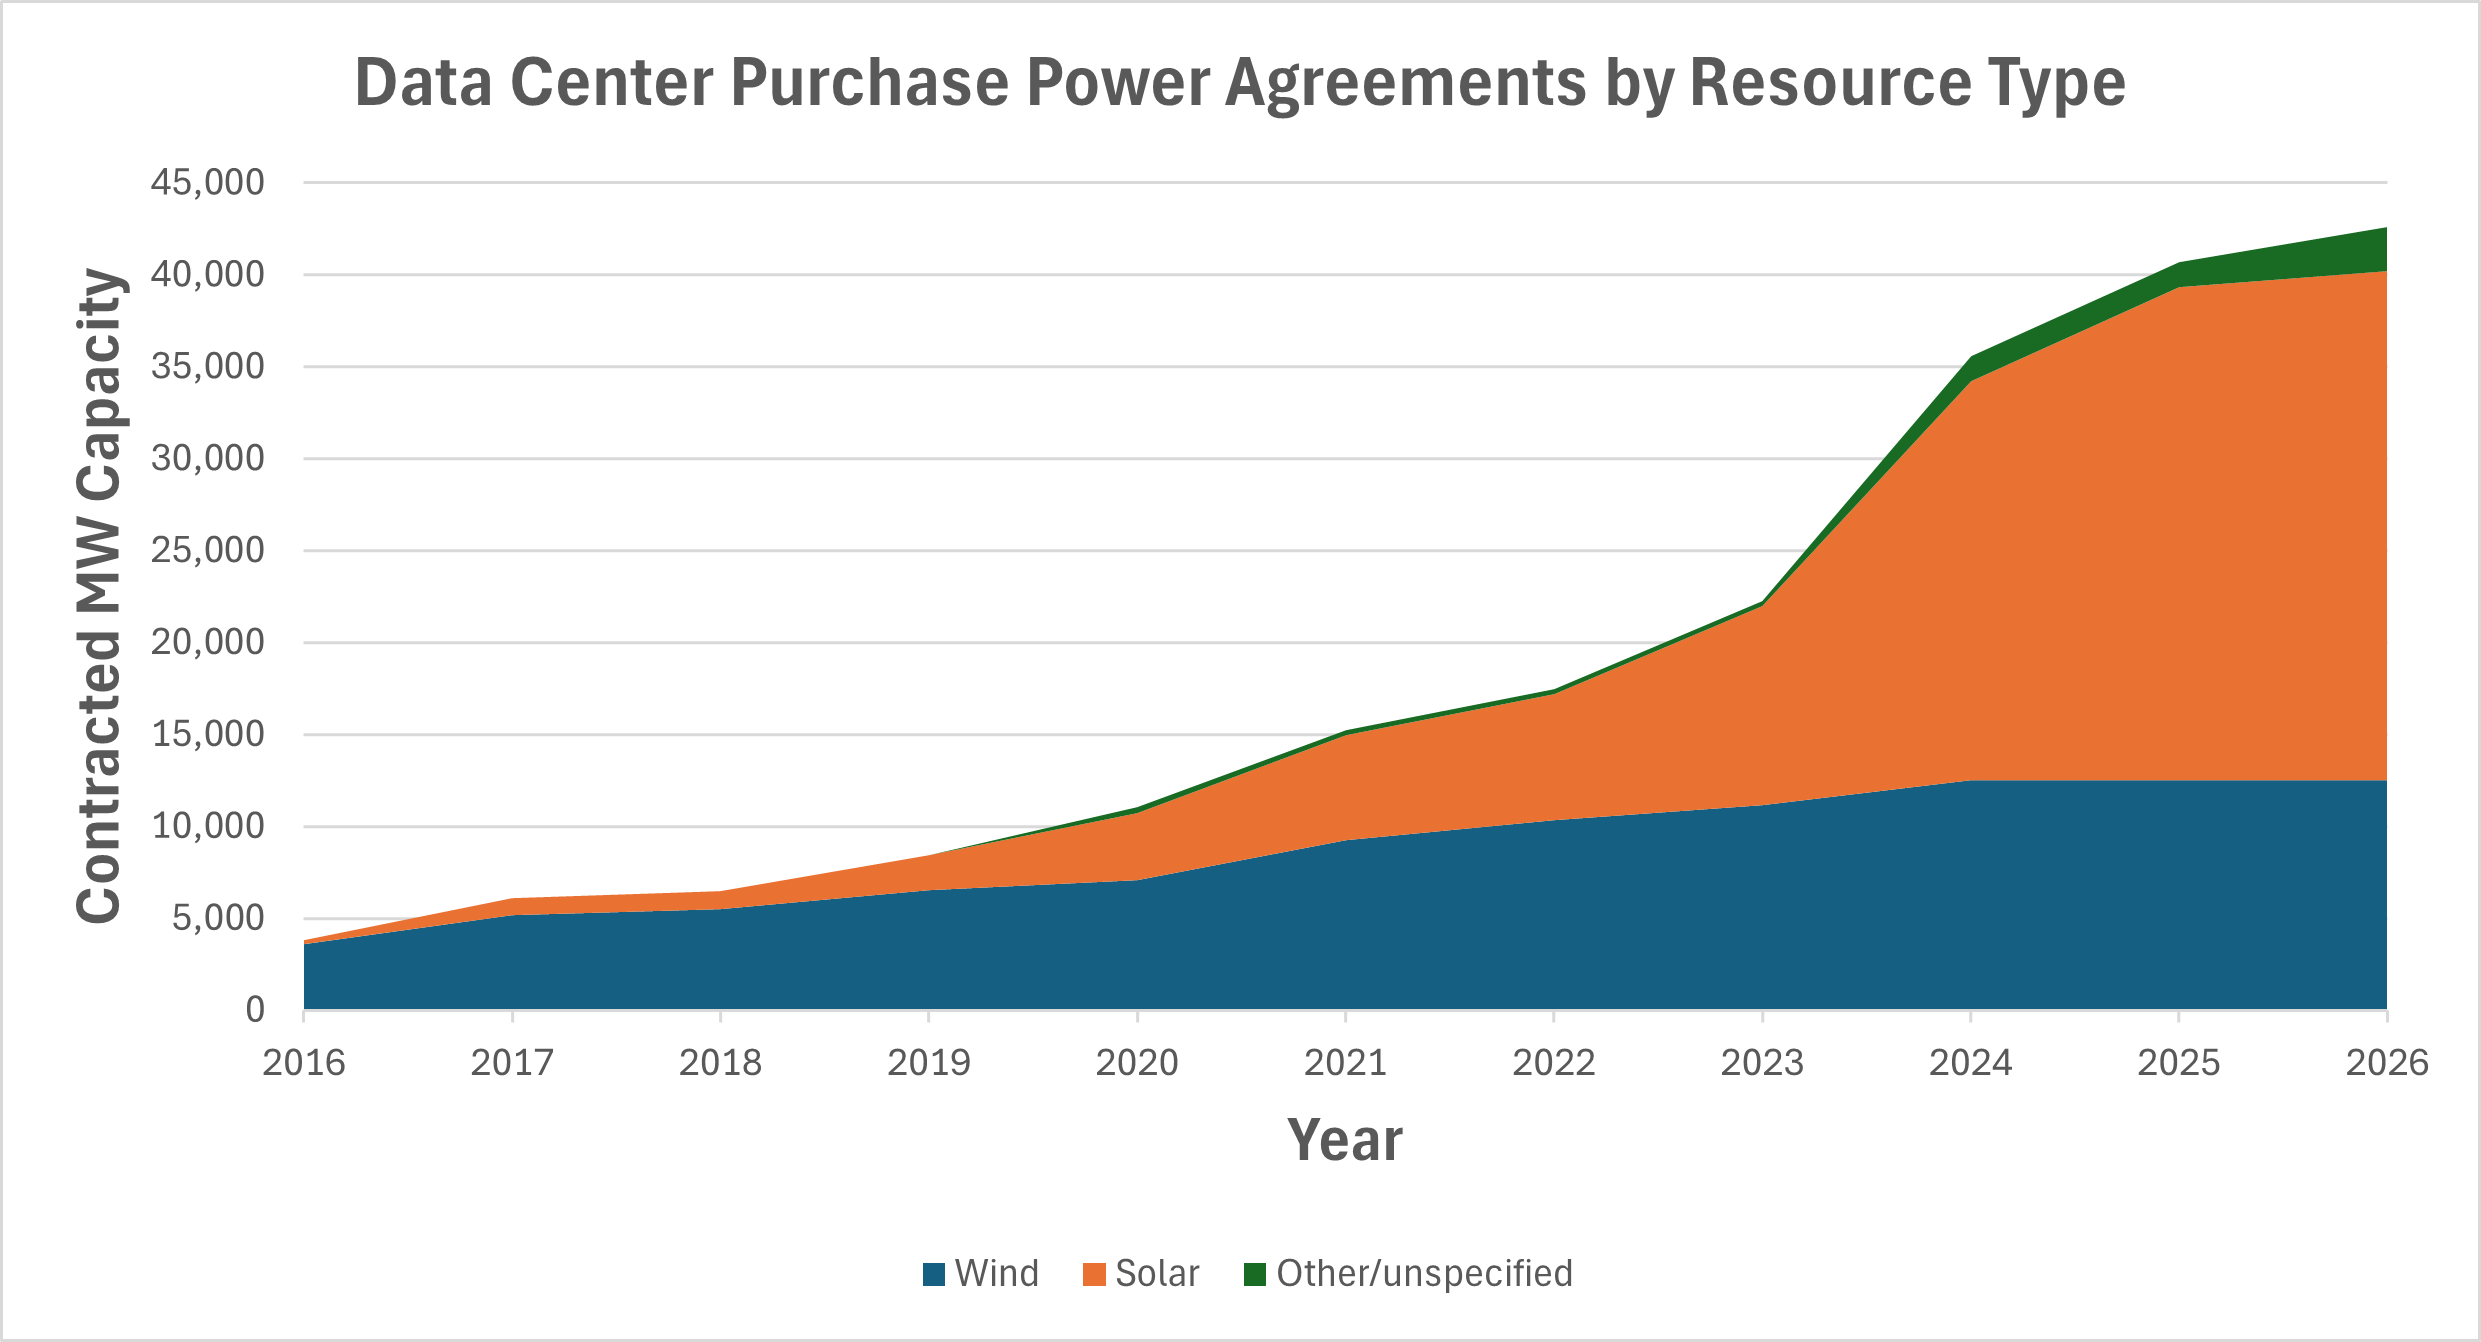
\includegraphics[width=0.75\linewidth]{Figures/PPA by Resource Type.png}
%     \caption{Data Center PPAs by Resource Type}
%     \label{fig:PPAbyResource}
% \end{figure}

% \begin{figure}
%     \centering
%     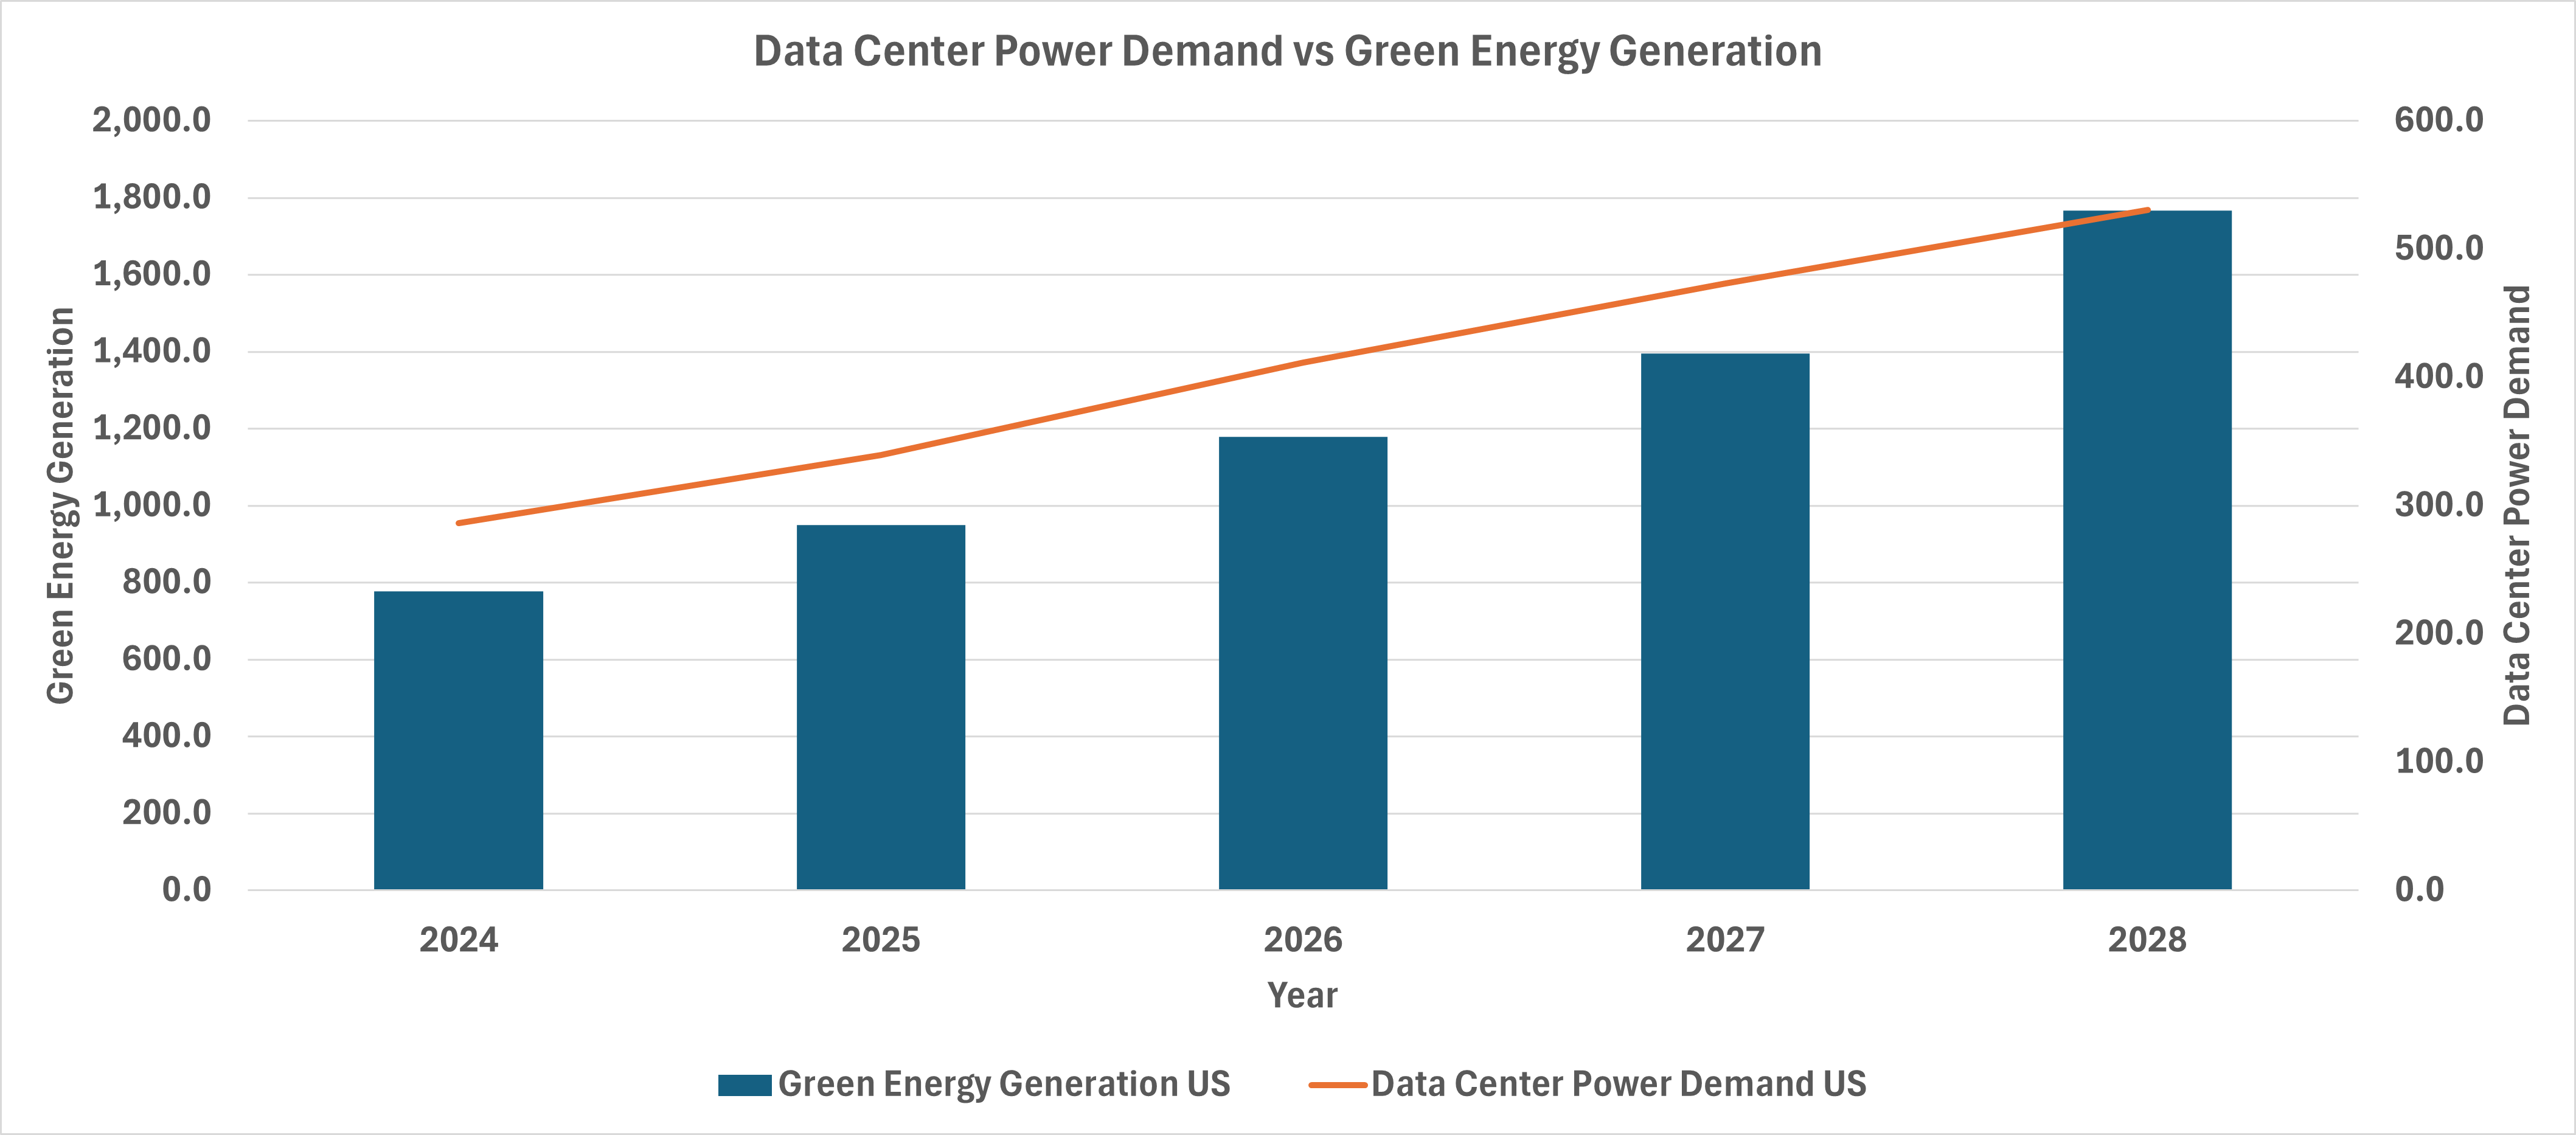
\includegraphics[width=0.5\linewidth]{Figures/Data Center Power Demand vs Green Generation.png}
%     \caption{Data Center Power Consumption vs Green Generation. Source: Aterio.io}
%     \label{fig:DCPowerConsumption}


\section{Results}\label{Sec::Results}
Our stacked DiD estimator (\autoref{subsec:eventstudy}) addresses potential bias from treatment effect heterogeneity in settings with staggered AI model releases. For all power quality and fossil demand effects, following \citet{callaway2021difference}, we construct cohort-specific datasets for each of the treatment events corresponding to major AI model publications through 2023, then stack these datasets to estimate a set of treatment effects across all dimensions. Table \ref{tab:combined_results} provides a full set of results from our main regressions including analysis of the impacts of on-site colocated generation for our counterfactuals.
%\nb{wouldnt know what these are at this point. Are these the $\beta_k$s?}. We compute price effects based on fossil demand effects.
% We estimate the effect of AI model deployment on electricity demand and power quality using a stacked difference-in-differences framework that addresses two identification challenges: (1) heterogeneous treatment timing across AI model releases, and (2) potential confounding from supply-side shocks that simultaneously affect electricity prices and quantities. Our primary specifications employ stacked event-study estimation, which allows us to trace out dynamic treatment effects and assess pre-trends. For power quality outcomes, where sample size constraints limit event-study precision, we supplement with two-way fixed effects (strict DiD) specifications that pool pre- and post-treatment periods into binary indicators. We then present robustness checks using alternative treatment definitions, followed by counterfactual exercises that explore how alternative evolutionary paths for AI compute might affect grid outcomes.


\subsection{Power Quality Effects: Utility-Level Strict DiD}

%We complement the generator-level demand analysis with an examination of power quality impacts at the utility service territory level. This analysis differs from the stacked event-study specification in several respects necessitated by data structure and sample size constraints.

%First, the unit of analysis shifts from individual generators to retail electric utility service territories (N = 71 utilities). Second, the outcome variables are the Consumer Power Quality Index (CPQI) and Total Harmonic Distortion (THD) rather than electricity demand. Third, treatment is defined as the presence of any AI-affiliated data center within the utility territory, rather than proximity to a specific facility. Fourth, the smaller sample size (1,136 utility-month observations) limits the precision of event-study coefficients, leading us to employ a strict two-way fixed effects (DiD) specification that pools pre- and post-treatment periods into binary indicators rather than tracing out event-time dynamics. We do not employ instrumental variables in this specification; the estimates capture the reduced-form relationship between AI data center presence and power quality outcomes.

%\subsubsection{Main Results}
We report the power quality effects of AI data centers in seventy one retail electric utility service territories estimated from power quality observations over 1136 utility-months. We use Consumer Power Quality Index (CPQI) and Total Harmonic Distortion (THD) as outcome variables in our stacked DiD models (~\autoref{eq:pq_eventstudy}). 

Table~\ref{tab:combined_results} reports results from the utility-level strict DiD specification. The CPQI coefficient speaks to the reliability of the power supply to the consumers. The CPQI coefficient of 0.3795 indicates a deterioration level that corresponds to moving from a typical U.S. power area toward the bottom quartile of power quality—roughly \textbf{the difference between $\sim$ 1 outage/year and $\sim$ 1.5–2 outages/year for the average customer}.Other reliability events such as brownouts and surges are predicted to increase by ~1-2 per year. Importantly, power surges are a known ignition source for electrical fires, contributing to the approximately 51,000 annual residential electrical fires in the U.S., with electrical arcing accounting for 74\% of ignition sources \cite{usfa2019electrical}. Fewer fires is generally considered a desirable outcome amongst electricity professionals \cite{Laughner2024THD}.
%\nb{Add brownouts or other reliability events}
\footnote{These are calculated based on Whisker Labs description of the CPQI Score with a description of derivation in the appendix.} This implies more frequent voltage anomalies that make motors and electronics run less efficiently and age faster.



The post-treatment coefficient of 0.0625 for THD indicates that utility territories containing AI data centers experienced a 0.0625 percentage point increase in readings above the 0.8 distortion threshold following AI model releases. 
%\nb{A 0.06\% increase reads negligible. Can we add something that makes the impact clearer, likely, and concrete. For example you could say: While a fraction of a percentage point might seem a negligible effect, in practice this level of increase can cause substantial problems. For example, this level of increase will halve the lifespan of ....} 
While a 0.0625 percentage point increase may appear small in isolation, the IEEE 519 standard exists precisely because even modest increases in harmonic distortion impose continuous thermal stress on motor windings. According to the Arrhenius equation underlying motor insulation ratings, every 10°C rise in operating temperature halves insulation life \cite{NEMA_MG1}. Since elevated THD causes motors to waste additional power as heat in their iron and copper windings \cite{Laughner2024THD}, sustained exposure compounds over the multi-year lifespans of household appliances, accelerating degradation of refrigerators, air conditioners, and other motor-driven equipment.

%(\nb{e.g. reducing the lifespan of a microwave by X}).

%indicates that the surrounding area can expect an additional reliability event per year. This level of deterioration in CPQI corresponds to moving from a typical U.S. area toward the bottom quartile of power quality—roughly \textbf{the difference between $\sim$ 1 outage/year and $\sim$ 1.5–2 outages/year for the average customer}\footnote{These are calculated based on Whisker Labs description of the CPQI Score with a description of derivation in the appendix.}—and implies more frequent voltage anomalies that make motors and electronics run less efficiently and age faster. \nb{Can we also add something about how much faster a specific appliance (say a microwave) could age under this level of power quality deterioration?}


% \begin{table}[h]
% \centering
% \caption{Utility-Level Power Quality Results: Two-Way Fixed Effects (Strict DiD) along with the quality of fit metric ($R^2$).  \nb{Get rid of N and SE}}
% \label{tab:thd_results}
% \begin{tabular}{lcccc}
% \toprule
% Outcome & Post Coefficient & SE & $R^2$ & N \\
% \midrule
% THD ($>$0.8 threshold) & 0.0625*** & $<$0.001 & 0.956 & 1,136 \\
% CPQI & 0.3795*** & $<$0.001 & 0.956 & 1,136 \\
% \bottomrule
% \end{tabular}
% \begin{flushleft}
% \footnotesize\textit{Notes:} *** p < 0.001. Utility and time fixed effects with cluster-robust standard errors. Treatment defined as presence of AI-affiliated data center in utility service territory.
% \end{flushleft}
% \end{table}

\subsection{Fossil Fuel Demand Effects: Stacked DiD Estimation}

We estimate Fossil Fuel Demand effects using demand data from a total of 35.6 million generator-hour observations, which includes 900,956 treated observations from generators located within 20 miles of AI-affiliated data centers and the other 34.7 million from other generators as control observations.

%\nb{move this to the robustness results and change table 3. Expand, at least once, OLS and 2SLS. Better yet unify terminology.}
We estimate the baseline specification via two-stage least squares (2SLS) to isolate demand-side effects from supply shocks. All specifications include zone and month fixed effects with standard errors clustered by unit-event. Further details on the instrumental variables specification can be found in Appendix Subsection \ref{IVDetails}. Table~\ref{tab:combined_results} reports the full stacked DiD coefficients.

% \nb{Change to new terminology. No event-study anymore.}
\paragraph{Stacked DiD Coefficients: OLS versus 2SLS.} Table~\ref{tab:combined_results} reports the full stacked DiD coefficients from both specifications. Figure \ref{fig:event_study_main} shows the stacked DiD coefficients for power demand in the 2SLS specification. The $t=+2$ coefficient shows a significant demand increase of 5.20 MWh, representing the demand shift at generators near data centers two months after AI model release, isolated from supply-side price variation through our instrumentation strategy. The pre-treatment coefficient at $t=-2$ is highly significant, representing demand created by training. While these effects may not seem large enough to be economically interesting, these effects are hourly and by generator. When the aggregate impact is calculated, they represent over 500 additional GWh added nearby to a data center over the inference period in some cases. \textbf{The additional power is roughly equivalent to that of 47,000 household-years in the United States}.

% \begin{table}[h]
% \centering
% \caption{Stacked DiD Coefficients: Generator-Level Demand}
% \label{tab:event_study}
% \begin{tabular}{lccccc}
% \toprule
% & \multicolumn{2}{c}{OLS} & & \multicolumn{2}{c}{IV 2SLS} \\
% \cmidrule{2-3} \cmidrule{5-6}
% Event Time & Coefficient & SE & & Coefficient & SE \\
% \midrule
% $t = -2$ & +1.28 & (1.29) & & +6.33*** & (1.63) \\
% $t = -1$ & \multicolumn{2}{c}{[reference]} & & \multicolumn{2}{c}{[reference]} \\
% $t = 0$ & $-4.39$ & (3.10) & & +0.69 & (2.79) \\
% $t = +1$ & $-1.64$ & (2.80) & & +0.74 & (2.45) \\
% $t = +2$ & +1.31 & (2.27) & & +5.20** & (2.54) \\
% \midrule
% Pre-treatment avg & \multicolumn{2}{c}{+1.28} & & \multicolumn{2}{c}{+6.33} \\
% Post-treatment avg & \multicolumn{2}{c}{$-1.57$} & & \multicolumn{2}{c}{+2.21} \\
% \bottomrule
% \end{tabular}
% \begin{flushleft}
% \footnotesize\textit{Notes:} *** p < 0.01, ** p < 0.05. N = 35.6 million observations from 19 treatment events. Standard errors clustered by unit-event. IV instruments: natural gas price $\times$ zone-average heat rate.
% \end{flushleft}
% \end{table}

% The OLS specification shows no significant effects in any period, consistent with the parallel trends validation. Figure \ref{fig:event_study_main} shows the stacked DiD coefficients for power demand in the 2SLS specification. The 2SLS specification reveals two notable patterns. First, the $t=-2$ coefficient is significant (6.33, p < 0.01) indicating a significant traning demand increase.. Second, the $t=+2$ coefficient shows a significant demand increase of 5.20 MWh (SE = 2.54, p < 0.05), representing the demand shift at generators near data centers two months after AI model release, isolated from supply-side price variation through our instrumentation strategy. While these effects may not seem large enough to be economically interesting, these effects are hourly and by generator. When the aggregate impact is calculated, they represent over 500 additional GWh added nearby to a data center over the inference period in some cases. \textbf{The additional power is roughly equivalent to that of 47,000 household-years in the United States}. This further strains grids as the power is not evenly distributed across hours. The pre-treatment coefficient at $t=-2$ is significant, representing demand created by training, but prior to treatment, the trends are identical with the control sample. Figure~\ref{fig:event_study_main} displays stacked DiD coefficients for the pre-treatment and post-treatment windows from the OLS specification. 
\begin{figure}[th!]
    \centering
    % Note: Reference the actual output files from stacked_did_iv_results/
    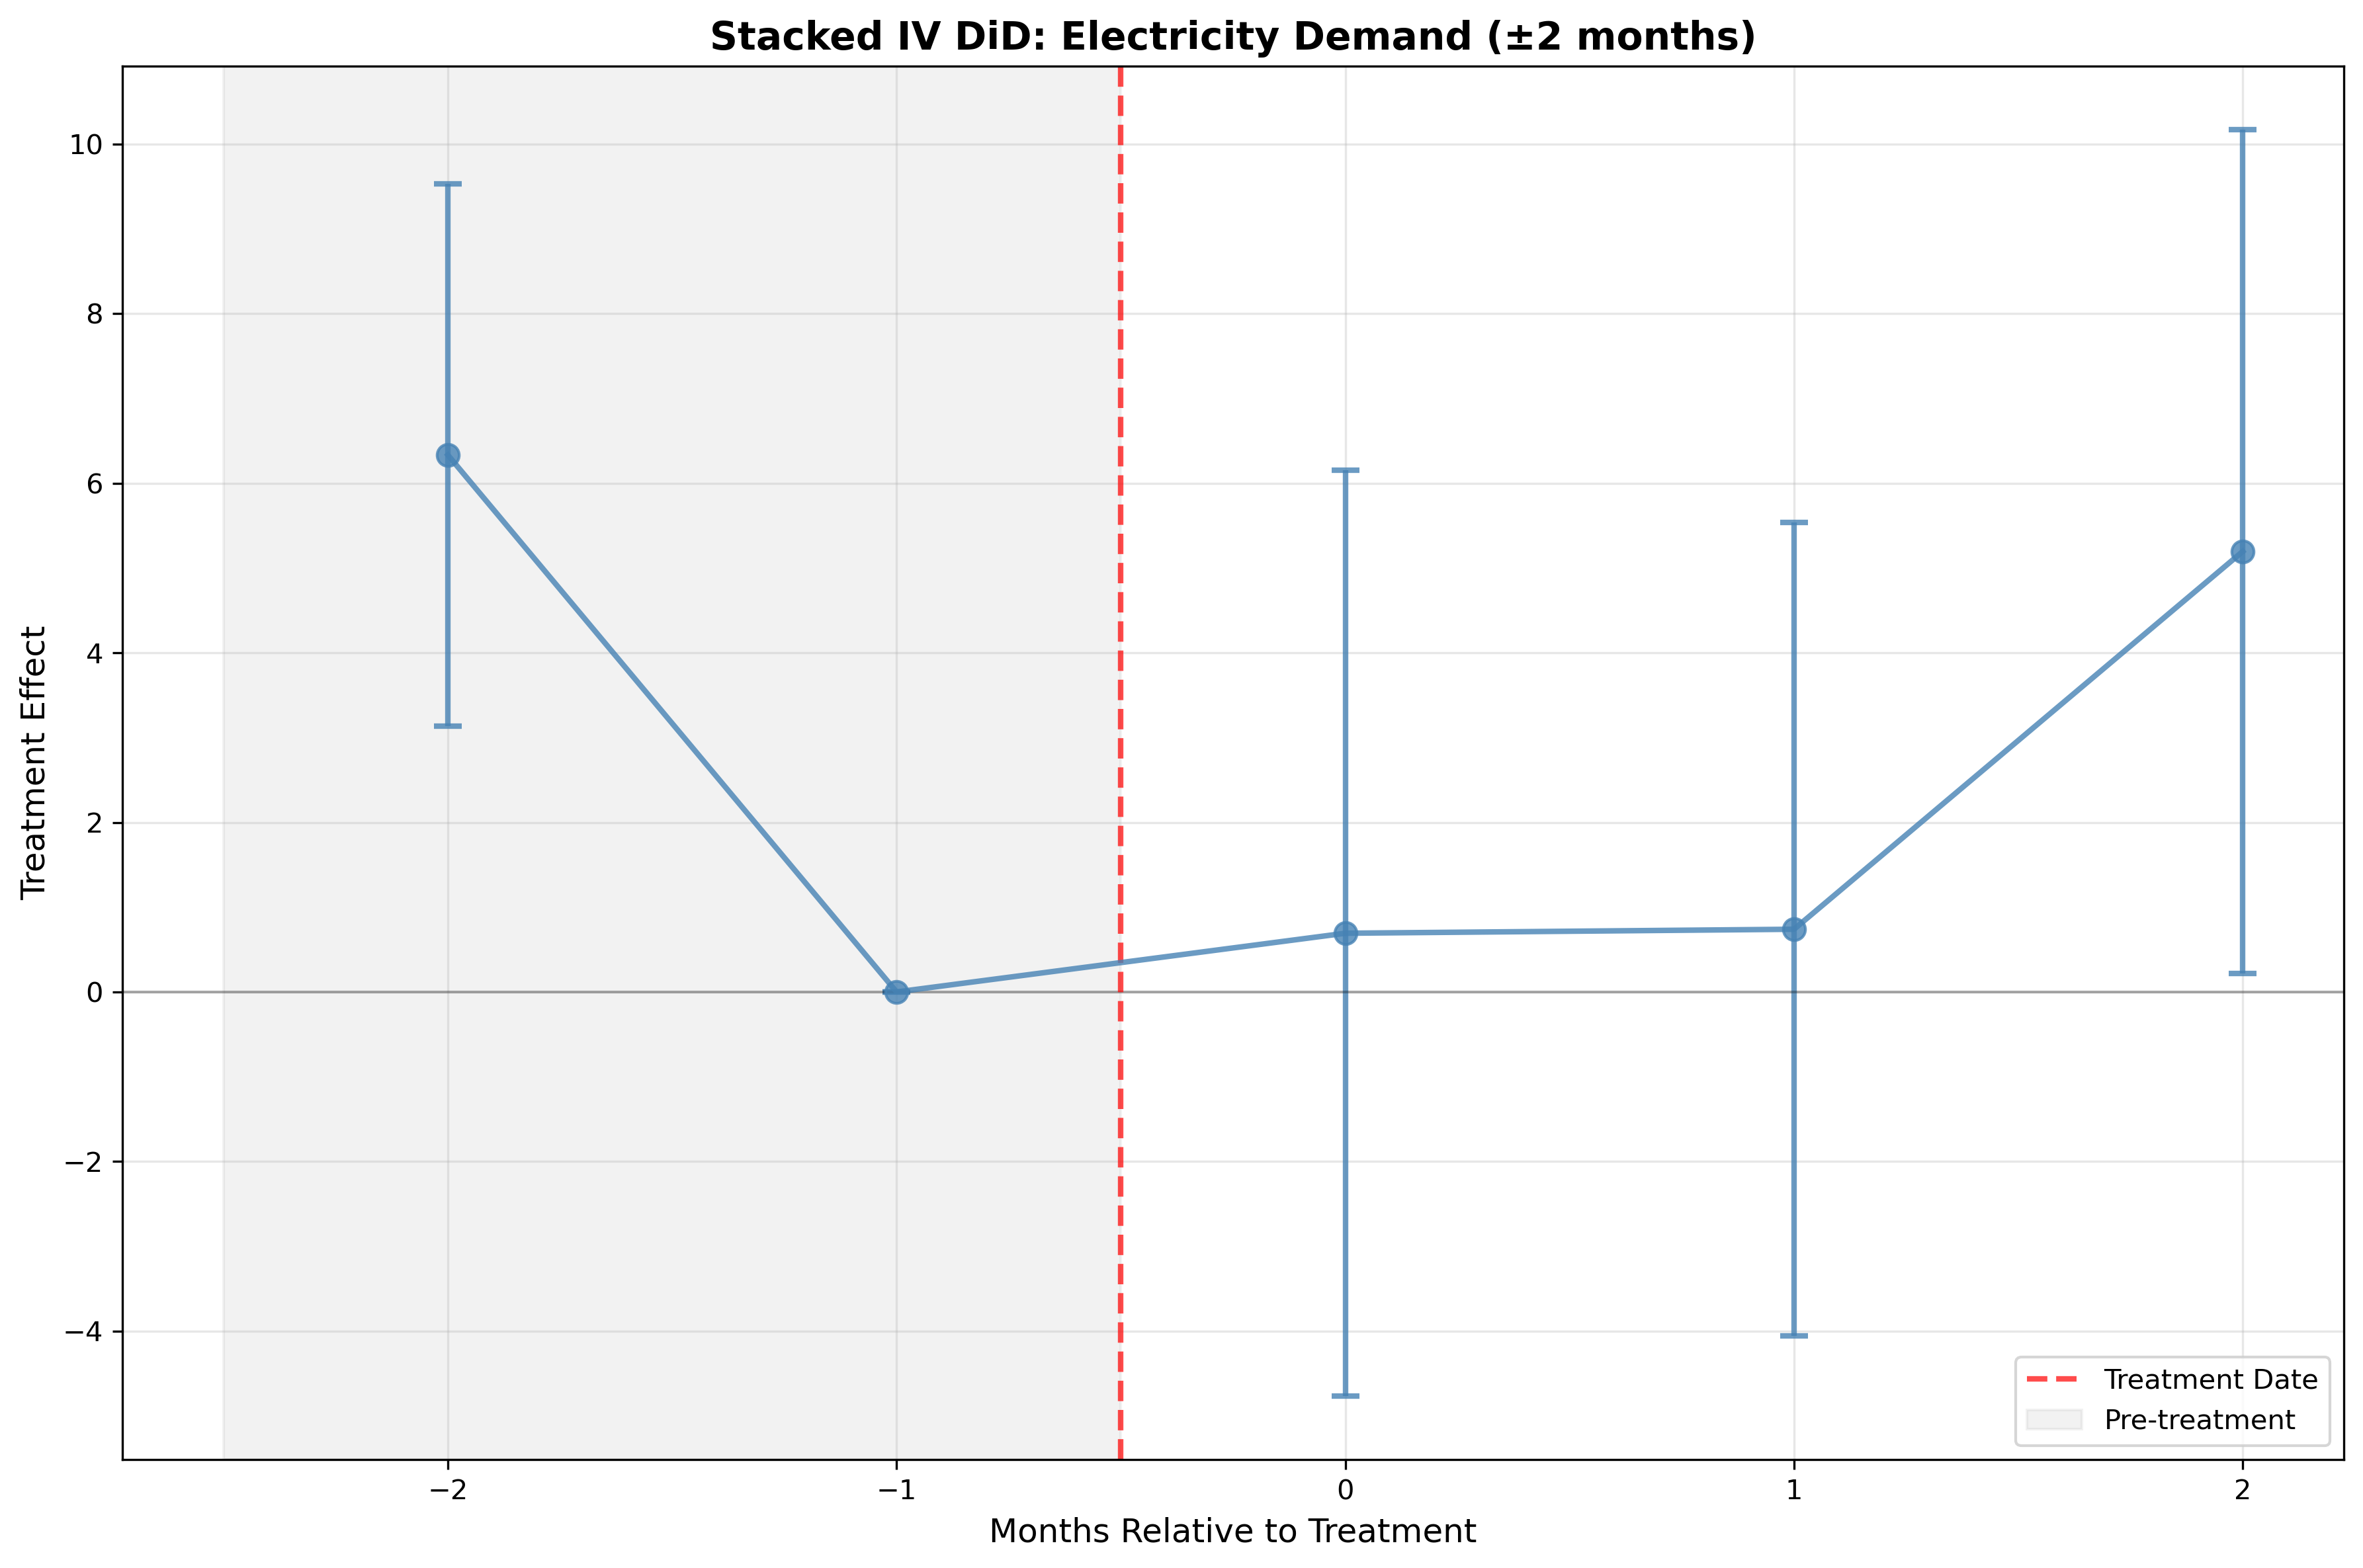
\includegraphics[width=0.8\linewidth]{Figures/event_study_iv.png}
    \caption{Stacked DiD coefficients for power demand (IV specification). Event Time 0 corresponds to AI model publication date. The pre-treatment coefficient at $t=-2$ demonstrates the training demand. Reference period is $t=-1$.}
    \label{fig:event_study_main}
\end{figure}

\begin{table*}[t]
\centering
\caption{Summary of Estimation Results Across Specifications}
\label{tab:combined_results}
\begin{tabular}{llcp{7.5cm}}
\toprule
Analysis & Outcome & Coefficient & Effect Interpretation \\
\midrule
\multicolumn{4}{l}{\textit{Panel A: Utility-Level Power Quality (Two-Way FE)}} \\
\addlinespace[0.5em]
Strict DiD & THD ($>$0.8) & 0.0625*** & More outages and equipment failure. \\
Strict DiD & CPQI & 0.3795*** & Moving from typical U.S. power quality to the bottom quartile; increases annual outages for the average customer from approximately 1 to 1.5–2. \\
\addlinespace[0.5em]
\midrule
\multicolumn{4}{l}{\textit{Panel B: Generator-Level Demand (Stacked DiD)}} \\
\addlinespace[0.5em]
OLS & Pre-treatment avg & +1.28 & \multirow{4}{7.5cm}{Aggregate impact represents over 500 additional GWh near data centers over the inference period—equivalent to $\sim$47,000 U.S. household-years of consumption, with load not evenly distributed across hours} \\
OLS & Post-treatment avg & $-1.57$ & \\
IV 2SLS & Pre-treatment avg & +6.33*** & \\
IV 2SLS & Post-treatment avg & +2.21 & \\
\addlinespace[0.5em]
\midrule
\multicolumn{4}{l}{\textit{Panel C: Power Quality by On-Site Generation Status}} \\
\addlinespace[0.5em]
With on-site & CPQI & $-0.122$*** & \multirow{3}{7.5cm}{On-site Generation generation mitigates grid stress from AI load; utilities without on-site experience reliability deterioration while those with on-site see improvements} \\
Without on-site & CPQI & +0.228*** & \\
Difference & CPQI & $-0.350$*** & \\
\bottomrule
\end{tabular}
\begin{flushleft}
\footnotesize\textit{Notes:} *** $p < 0.001$, ** $p < 0.05$. Panel A: Utility and time fixed effects with cluster-robust standard errors; treatment defined as presence of AI-affiliated data center in utility service territory. Panel B: 35.6 million observations from 19 treatment events; standard errors clustered by unit-event; IV instruments: natural gas price $\times$ zone-average heat rate. Panel C: CPQI = Consumer Power Quality Index; THD = Total Harmonic Distortion.
\end{flushleft}
\end{table*}


% \subsubsection{Parallel Trends Validation}

% We first assess the parallel trends assumption underlying our identification strategy.


\subsection{Price Impacts}

% We estimate wholesale electricity price impacts by combining our demand estimates with supply curve parameters, following the methodology outlined in Section \ref{PriceEffects}. This approach recognizes that our IV strategy identifies demand shifts but does not directly estimate equilibrium price effects\nb{expand this terminology as a footnote}. The price impact of AI-induced demand depends on the slope of the supply curve\nb{footnote explaining what this is}: inelastic supply\nb{expand this terminology} implies large price effects, while elastic supply implies small effects. Additional specifics on calculation methodology can be found in Appendix Subsection \ref{CalcMethodologyPrice}. 

We estimate wholesale electricity price impacts by combining our demand estimates with supply curve parameters, following the methodology outlined in Section \ref{PriceEffects}. This approach recognizes that our IV strategy identifies demand shifts but does not directly estimate equilibrium price effects.\footnote{Our instrumental variables approach isolates exogenous variation in electricity demand driven by AI model releases. However, observed market prices reflect the intersection of supply and demand in equilibrium. To translate our demand estimates into price effects, we must incorporate information about supply-side responses, which requires additional assumptions about the shape of the supply curve.} The price impact of AI-induced demand depends on the slope of the supply curve\footnote{The supply curve describes the relationship between price and quantity supplied. Its slope reflects how much generators must be compensated to produce additional electricity—steeper slopes indicate that marginal generation costs rise quickly as output expands, typically because higher-cost units must be dispatched.}: inelastic supply—where quantity supplied responds weakly to price changes—implies large price effects, while elastic supply implies small effects. Additional specifics on calculation methodology can be found in Appendix Subsection \ref{CalcMethodologyPrice}.

A map of estimated supply chain elasticities can be found in Figure \ref{PJMPRiceElasticity} in Appendix section \ref{PriceElasticityAppendix} demonstrates the supply elasticity by zone in PJM. Figure \ref{PJMPrice} showing price increase estimates by zone. On average AI training leads to \textbf{substantial increases in wholesale prices in PJM with the highest increase surpassing 25\% in the American Electric Power (AEP) Zone}. Additional caveats are provided in Appendix Subsection \ref{appendix:Caveats}

\begin{figure}
    \centering
    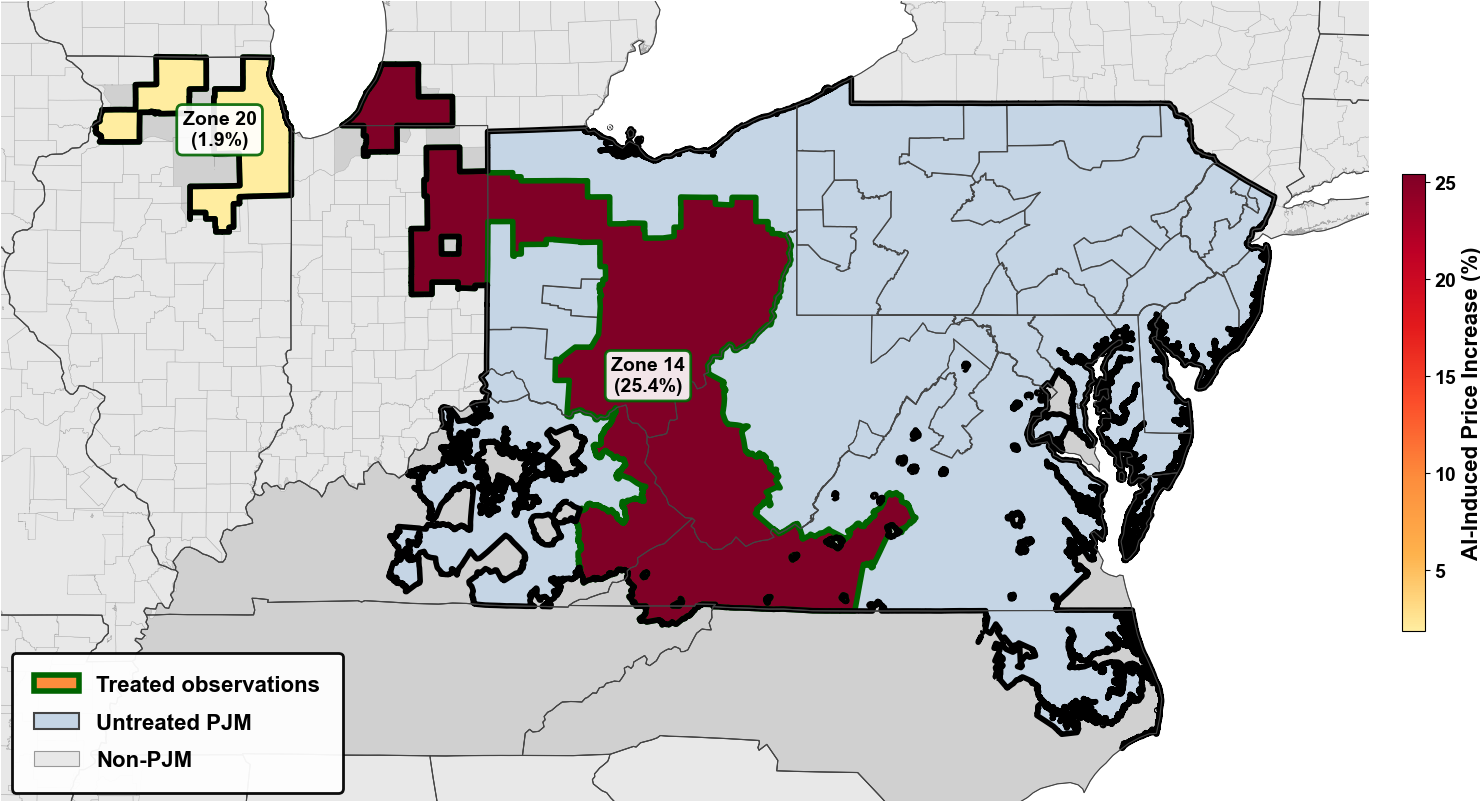
\includegraphics[width=0.75\linewidth]{Figures/PJMMap3.png}
    \caption{Price Effects of AI in PJM.}
    \label{PJMPrice}
\end{figure}

While we are not able to provide definite evidence of the impacts on retail price pass through, it should be noted that retail electricity prices have increased overall at a rate surpassing inflation since 2020 \cite{Nicoletti_Malik_Tartar_2024,horsley2025electricbill,spp2024stateofthemarket}. While it is possible that increased investment in electric generation through power purchase agreements by tech firms may in the long run lead to falling retail prices, it appears that at present data center power usage is increasing wholesale prices by raising total demand, which requires dispatching higher-cost generators and thus increases the market clearing price—a price paid by all retail consumers.

Using estimates from the literature as documented in Appendix Subsection \ref{WholesaleRetailPassthrough}, we can bracket the expected price rise for retail consumers. Two recent estimates apply but speak to different horizons. \cite{defeuilley2023pennsylvania} report short-run passthrough of roughly $0.53$--$0.56$ in PJM/Pennsylvania over a sample window dominated by short retail-rate refresh cycles and explicit fuel-cost-adjustment provisions; applying that passthrough to a 25\% wholesale shock in AEP implies a short-run consumer price rise of roughly 13\%. \cite{mackay2024wholesale} estimate long-run passthrough closer to one across U.S.\ retail markets, on the assumption that procurement contracts, default-service auctions, and rate-case filings eventually fully reflect sustained wholesale movements; under that estimate the long-run consumer price rise approaches the full 25\%. The two numbers therefore correspond to short-run vs.\ long-run passthrough rather than to competing estimates of the same object: the 13\% figure is the appropriate near-term magnitude for retail bills under existing PJM rate mechanics, while the 25\% figure is the appropriate long-run magnitude if the wholesale shock is sustained for several rate cycles. We report both and let the reader weight them according to the policy horizon of interest, rather than collapsing to a single point estimate.
\section{Validating Assumptions and Robustness Checks}\label{Robustness}
% \nb{refer to earlier mention of issues}
We conduct several additional analyses to probe the robustness of our findings and explore effect heterogeneity in order to address issues highlighted in Subsection \ref{DCASSUmptions}. The formal testing helps provide evidence for the parallel trends assumption while the placebo tests address potential issues related to external confounds or lack of specific knowledge about training. Additional robustness analyses can be found in Appendix Subsection \ref{App:AdditionalRobustnessChecks}.

\subsubsection{Formal Testing for Parallel Trends}

 For power demand specifically, the formal joint test of pre-treatment coefficients yields a chi-squared statistic of 0.99 (df = 1) with p-value = 0.3196. \textbf{We cannot reject the null hypothesis of parallel pre-trends at conventional significance levels.} This provides support for our identification assumption: treated and control generators followed similar demand trajectories prior to AI model releases. Some of our samples demonstrate significant evidence against the the parallel trends test prior to propensity score matching. However, in 100\% of our samples for both power quality and power demand after propensity score matching, we \textit{fail to reject the null hypothesis of }. This implies that the technique correctly handles the issue where it exists. 
 
 Additionally, We estimate the baseline specification via OLS to validate parallel trends prior to implementing our instrumental variables strategy. The OLS specification shows no significant effects in any period outside the training window, consistent with parallel trends holding in the pre-treatment period. Importantly, prior to treatment (excluding $t=-2$, which captures training demand), the trends are identical between treatment and control samples. Figure~\ref{fig:event_study_main} displays stacked DiD coefficients for both pre-treatment and post-treatment windows, with the reference period at $t=-1$.

 \subsubsection{Placebo Tests}
We conduct three placebo exercises to assess the validity of our identification strategy. First, to distinguish AI-specific effects from general data center growth, we estimate treatment effects using our 12,283 non-AI data centers as a placebo treatment group. If estimated effects simply reflect data center proximity rather than AI workloads specifically, we would expect similar magnitudes in this specification. The non-AI CPQI coefficient (0.228, p < 0.001) matches the AI data center coefficient for facilities without on-site generation, suggesting that general data center load---not AI workloads specifically---drives some of the observed power quality effects. However, the demand-side 2SLS estimates from the stacked DiD, which leverage AI model release timing, remain distinct from this general data center effect.

Second, we implement random date and random location placebo tests. Both yield a p-value of 1.00 for the coefficient in our fossil fuel demand, CPQI, and THD analyses, confirming that our results do not arise from spuriously chosen locations or dates.

% \subsubsection{Non-AI Data Center Placebo}

% To distinguish AI-specific effects from general data center growth, we estimate treatment effects using our 12,283 non-AI data centers as a placebo treatment group. If estimated effects simply reflect data center proximity rather than AI workloads specifically, we would expect similar magnitudes in this specification.

% The non-AI CPQI coefficient (0.228, p < 0.001) matches the AI data center coefficient for facilities without BTM generation, suggesting that general data center load---not AI workloads specifically---drives some of the observed power quality effects. However, the demand-side 2SLS estimates from the stacked event-study, which leverage AI model release timing, remain distinct from this general data center effect.

% \subsubsection{Random Dates and Random Locations Placebos}

% Both random dates and random locations yield a p-value of 1.00 for the coefficient in our fossil fuel demand, CPQI, and THD analyses. This suggests that our results are not the result of randomly chosen locations or dates.

\section{Counterfactual Analyses}
\label{sec:counterfactuals}

We present three main counterfactual exercises to inform stakeholders and policymakers about how alternative evolutionary paths for AI compute might affect grid outcomes. These combine our econometric estimates with data on model characteristics and infrastructure configurations to explore three dimensions: model scaling, geographic redistribution, and workload composition. Our counterfactual policies highly align with the implications of our theoretic model, particularly when considering the role of on-site generation as a solution to the challenges facing power procurement.\\

\noindent\textbf{1) Model Scaling.} We combine data on model size (parameter counts) with our econometric estimates from our least conservative specification to extrapolate grid impacts at different scales.

\noindent\textbf{(a) Power Quality.} Fitting a trend line to power quality impacts for Llama-3.1 (405B), PaLM (540B), and Llama 4 Behemoth (2T), we find that scaling from a 2 trillion parameter model to a 4 trillion parameter model would increase power quality impact from \textbf{0.321 to 0.434}---a deterioration of roughly 0.113 units, or just over 35\% relative to the 2 trillion baseline. The relationship is exponential over log parameter counts, implying that larger models require proportionally greater parameter reductions to achieve the same percentage improvement in power quality. \textbf{(b) Power Demand.} Using an analogous extrapolation, we find that \textbf{each 1\% parameter increase leads to approximately 0.15\% higher power demand} within three months of model release. Scaling from 540 billion to one trillion parameters would \textbf{increase total power demand by 10.5\%}. For DALL-E, halving parameters would \textbf{reduce inference demand by approximately 300 GWh}---equivalent to the annual consumption of 27,000--30,000 homes.\\

\noindent\textbf{2) Training Compute.} Training compute requirements also have measurable effects: a 1\% increase in training FLOPs is associated with a \textbf{0.1\% increase in power demand}. For GPT-3.5, halving training compute would reduce energy use by enough to power 8,000--10,000 U.S.\ homes for a year.\\

\noindent\textbf{3) Colocated On-site Generation.} Data centers increasingly deploy colocated on-site generation to reduce grid dependence. Our inventory identifies 87 facilities with on-site capability and 12,401 without. We test whether on-site capacity moderates estimated effects by interacting treatment with on-site status in the utility-level strict DiD specification. Results indicate that on-site generation substantially mitigates measured grid impacts. The sign reversal for CPQI is notable: data centers \textit{with} on-site generation are associated with improved power quality (negative coefficient), while those \textit{without} are associated with deterioration (positive coefficient). This heterogeneity suggests that \textbf{on-site generation absorbs demand spikes that would otherwise propagate to the grid}, and that aggregate grid impacts may understate total AI energy consumption.

Figure~\ref{fig:CounterfactualCombined} extends this to policy-relevant scenarios. Remarkably, universal adoption of on-site power would shift impact of data centers from a net detriment to power quality to a net improvement.\\
%However, all large AI data centers in our most conservative sample had on-site generation, which may exaggerate our estimates of colocated on-site generation's moderating effects.\nb{This statement again is a bit hard to parse. Does it undercut the impact statement above or support it?}

% \begin{figure}[h]
%     \centering
%     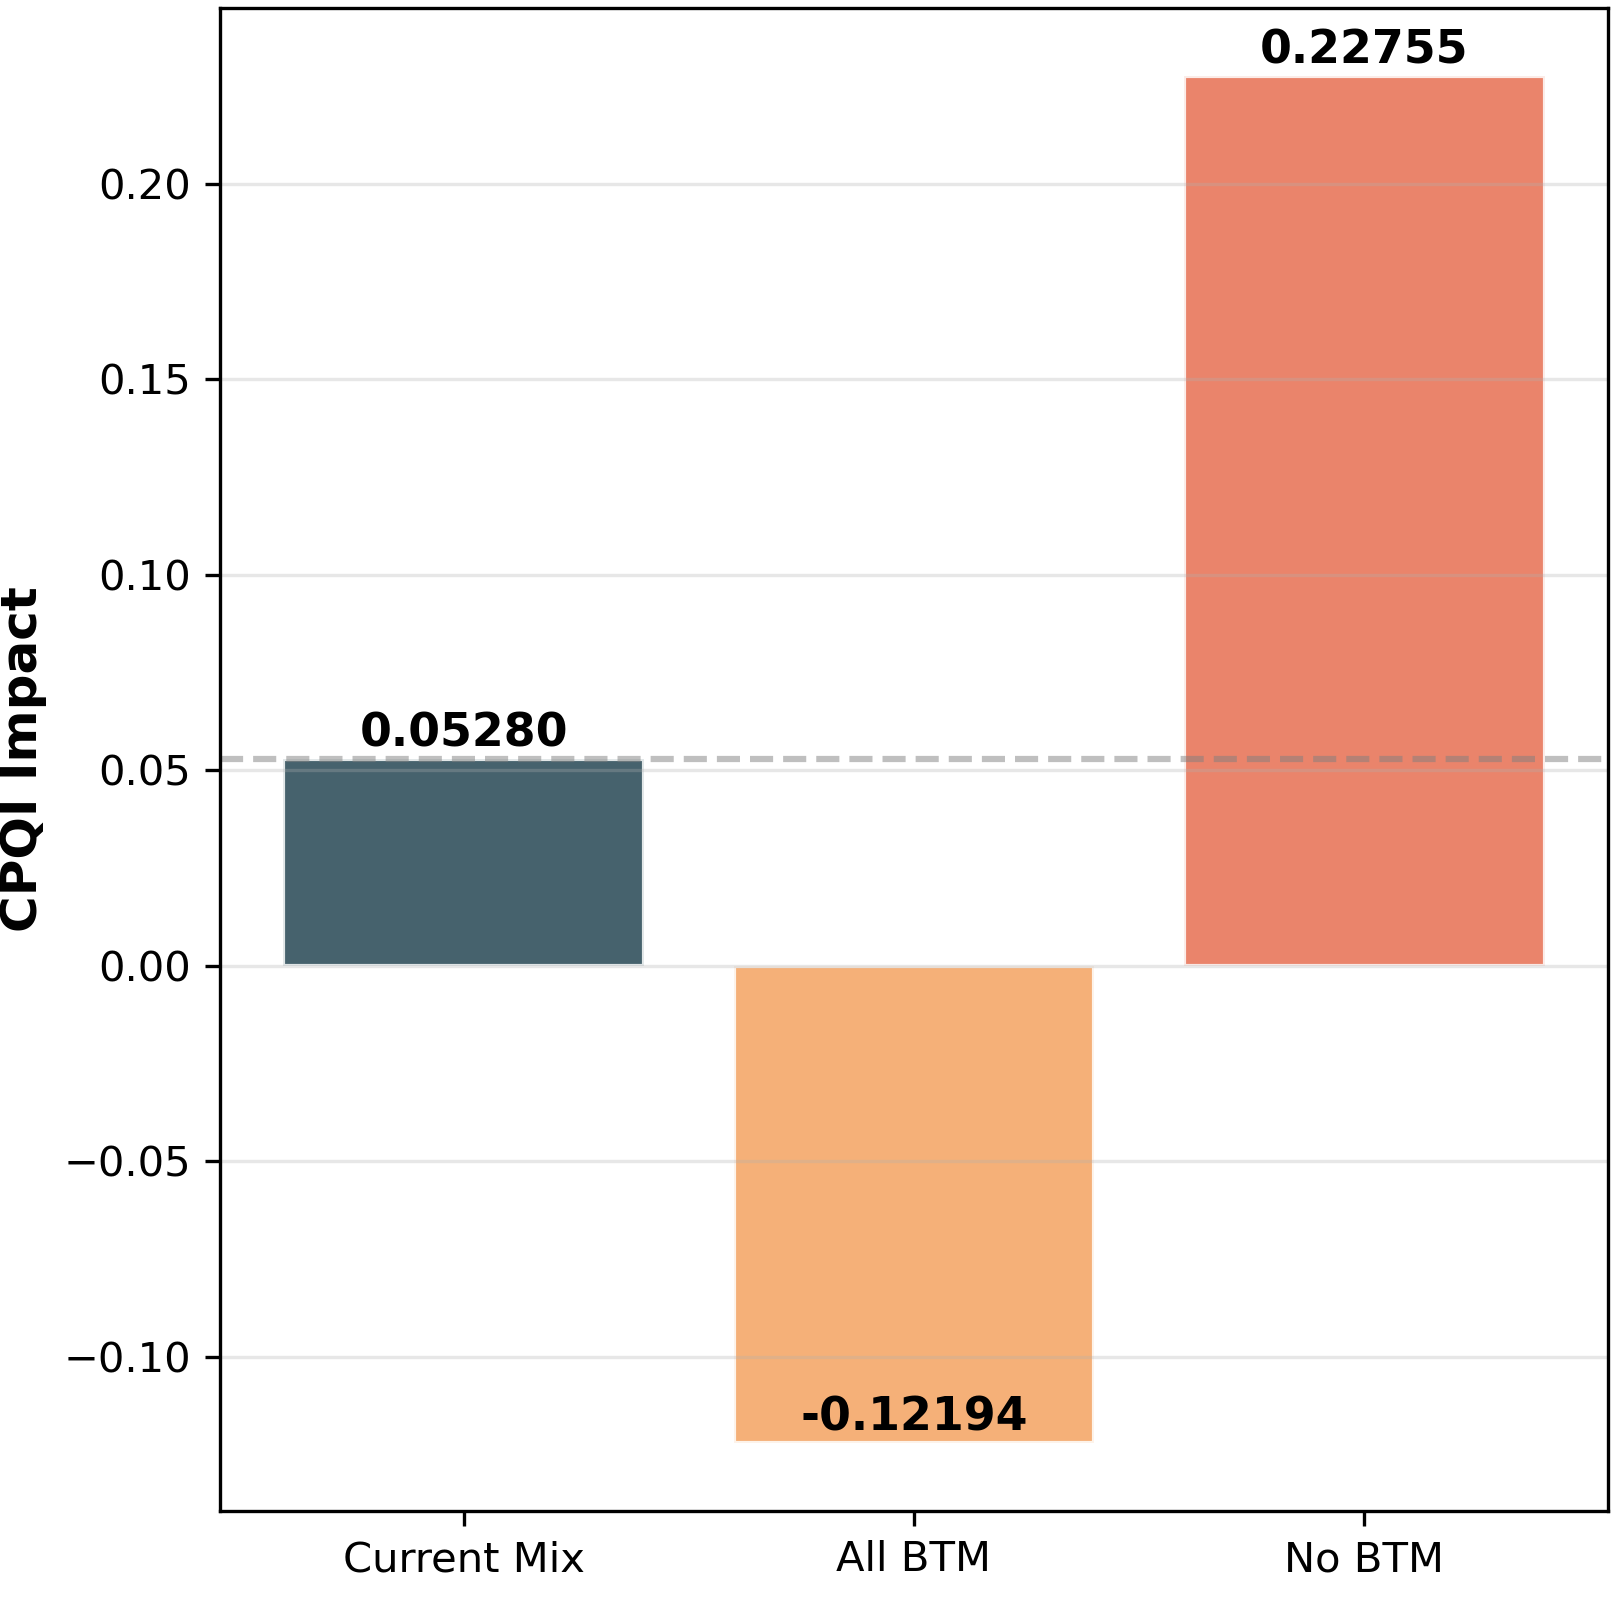
\includegraphics[width=0.35\linewidth]{Figures/btm_scenarios_analysis.png}
%     \caption{Impact of on-site power adoption on AI energy impacts.\nb{Dana it might be useful to collate plots in 5,6,and7 into a single figure laid side by side going across the two columns. this will save white space but also help make the figures bigger.}}
%     \label{fig:btm_scenarios}
% \end{figure}

\noindent\textbf{4) Geographic Redistribution}

%We analyze grid impacts under alternative spatial distributions of AI compute.

\noindent\textbf{(a) Distributed Inference (Edge Computing).} In our sample where we know AI data centers but not specific training and inference sites, we simulate a shift from cloud-based to edge-based inference, redistributing inference demand from concentrated hyperscaler facilities to smaller data centers located closer to population centers. Under this scenario, total demand added in a particular zone falls from a baseline of 162 MWh per hour over the entire treatment period to 4 MWh per hour. Figure ~\ref{fig:CounterfactualCombined} illustrates this effect of shifting the composition of inference.

% \begin{figure}[h]
%     \centering
%     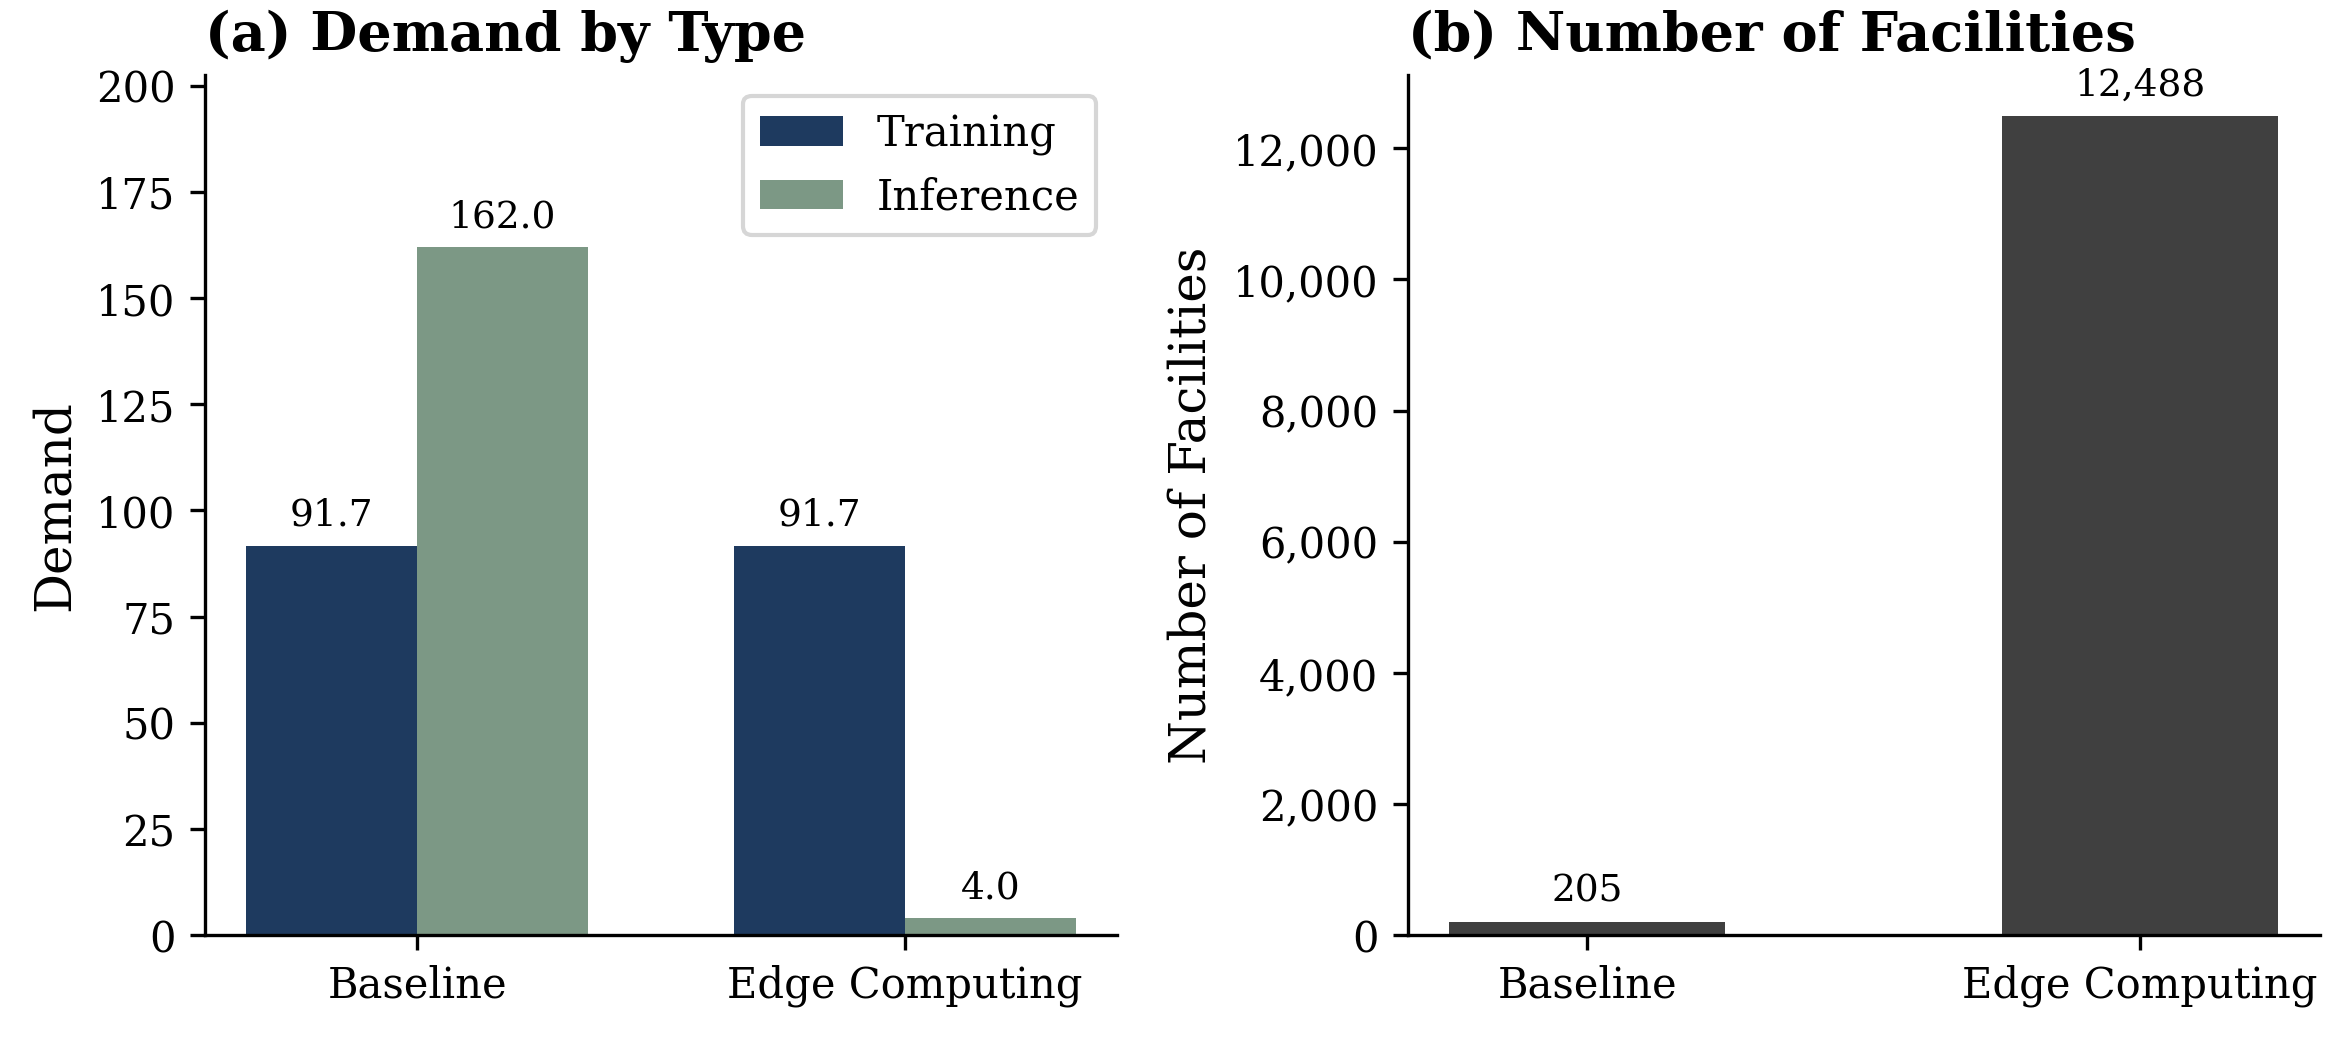
\includegraphics[width=0.5\linewidth]{Figures/CentralizedComputing.png}
%     \caption{Impact of distributing AI inference to edge data centers.}
%     \label{fig:edge_computing}
% \end{figure}

\noindent\textbf{(b) Concentration in Low-Population, High-Supply Regions.} Alternatively, we consider relocating both training and inference to regions with abundant electricity supply and lower baseline load, such as areas in the central United States with substantial renewable or fossil capacity. We simulate this by shifting demand from the baseline case where training and inference are assumed distributed to a case where the only data center for training and inference is the largest data center owned by a hyperscaler. This leads to an extreme concentration of added demand with nearly 100 GWh added near data centers in training locations. Figure~\ref{fig:CounterfactualCombined} shows this scenario.

This analysis has the important caveat that shifting to one data center for all training activity is extreme, with many possible configurations between full decentralization and full centralization. Centralization may also yield other benefits, such as concentration near renewable generation and reduced energy consumption from lower communication costs.

% \begin{figure}[h]
%     \centering
%     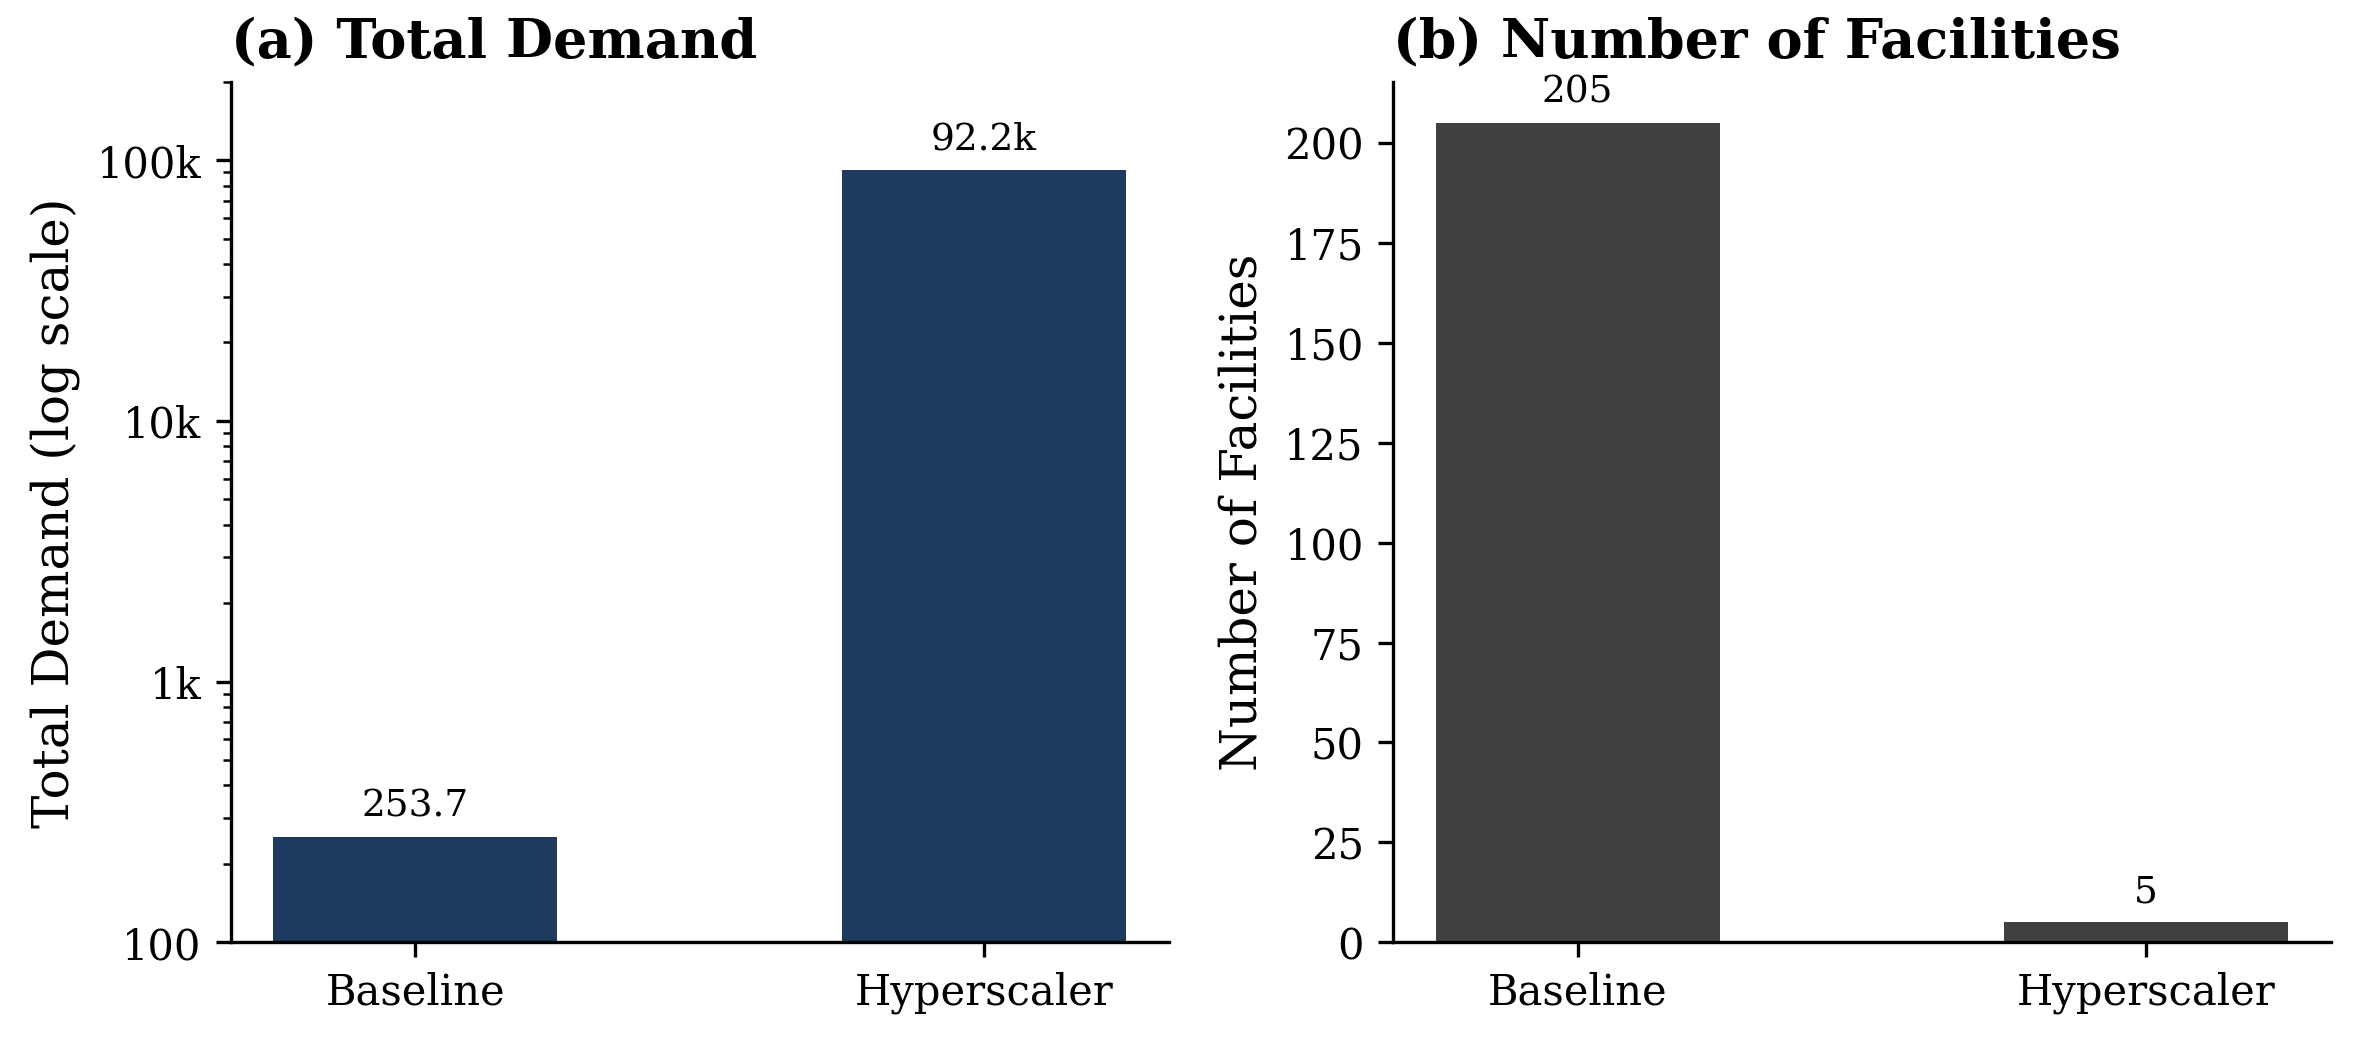
\includegraphics[width=0.5\linewidth]{Figures/Central.png}
%     \caption{Impacts of centralized computing to largest data center by hyperscaler.}
%     \label{fig:centralized_computing}
% \end{figure}

\begin{figure}
    \centering
    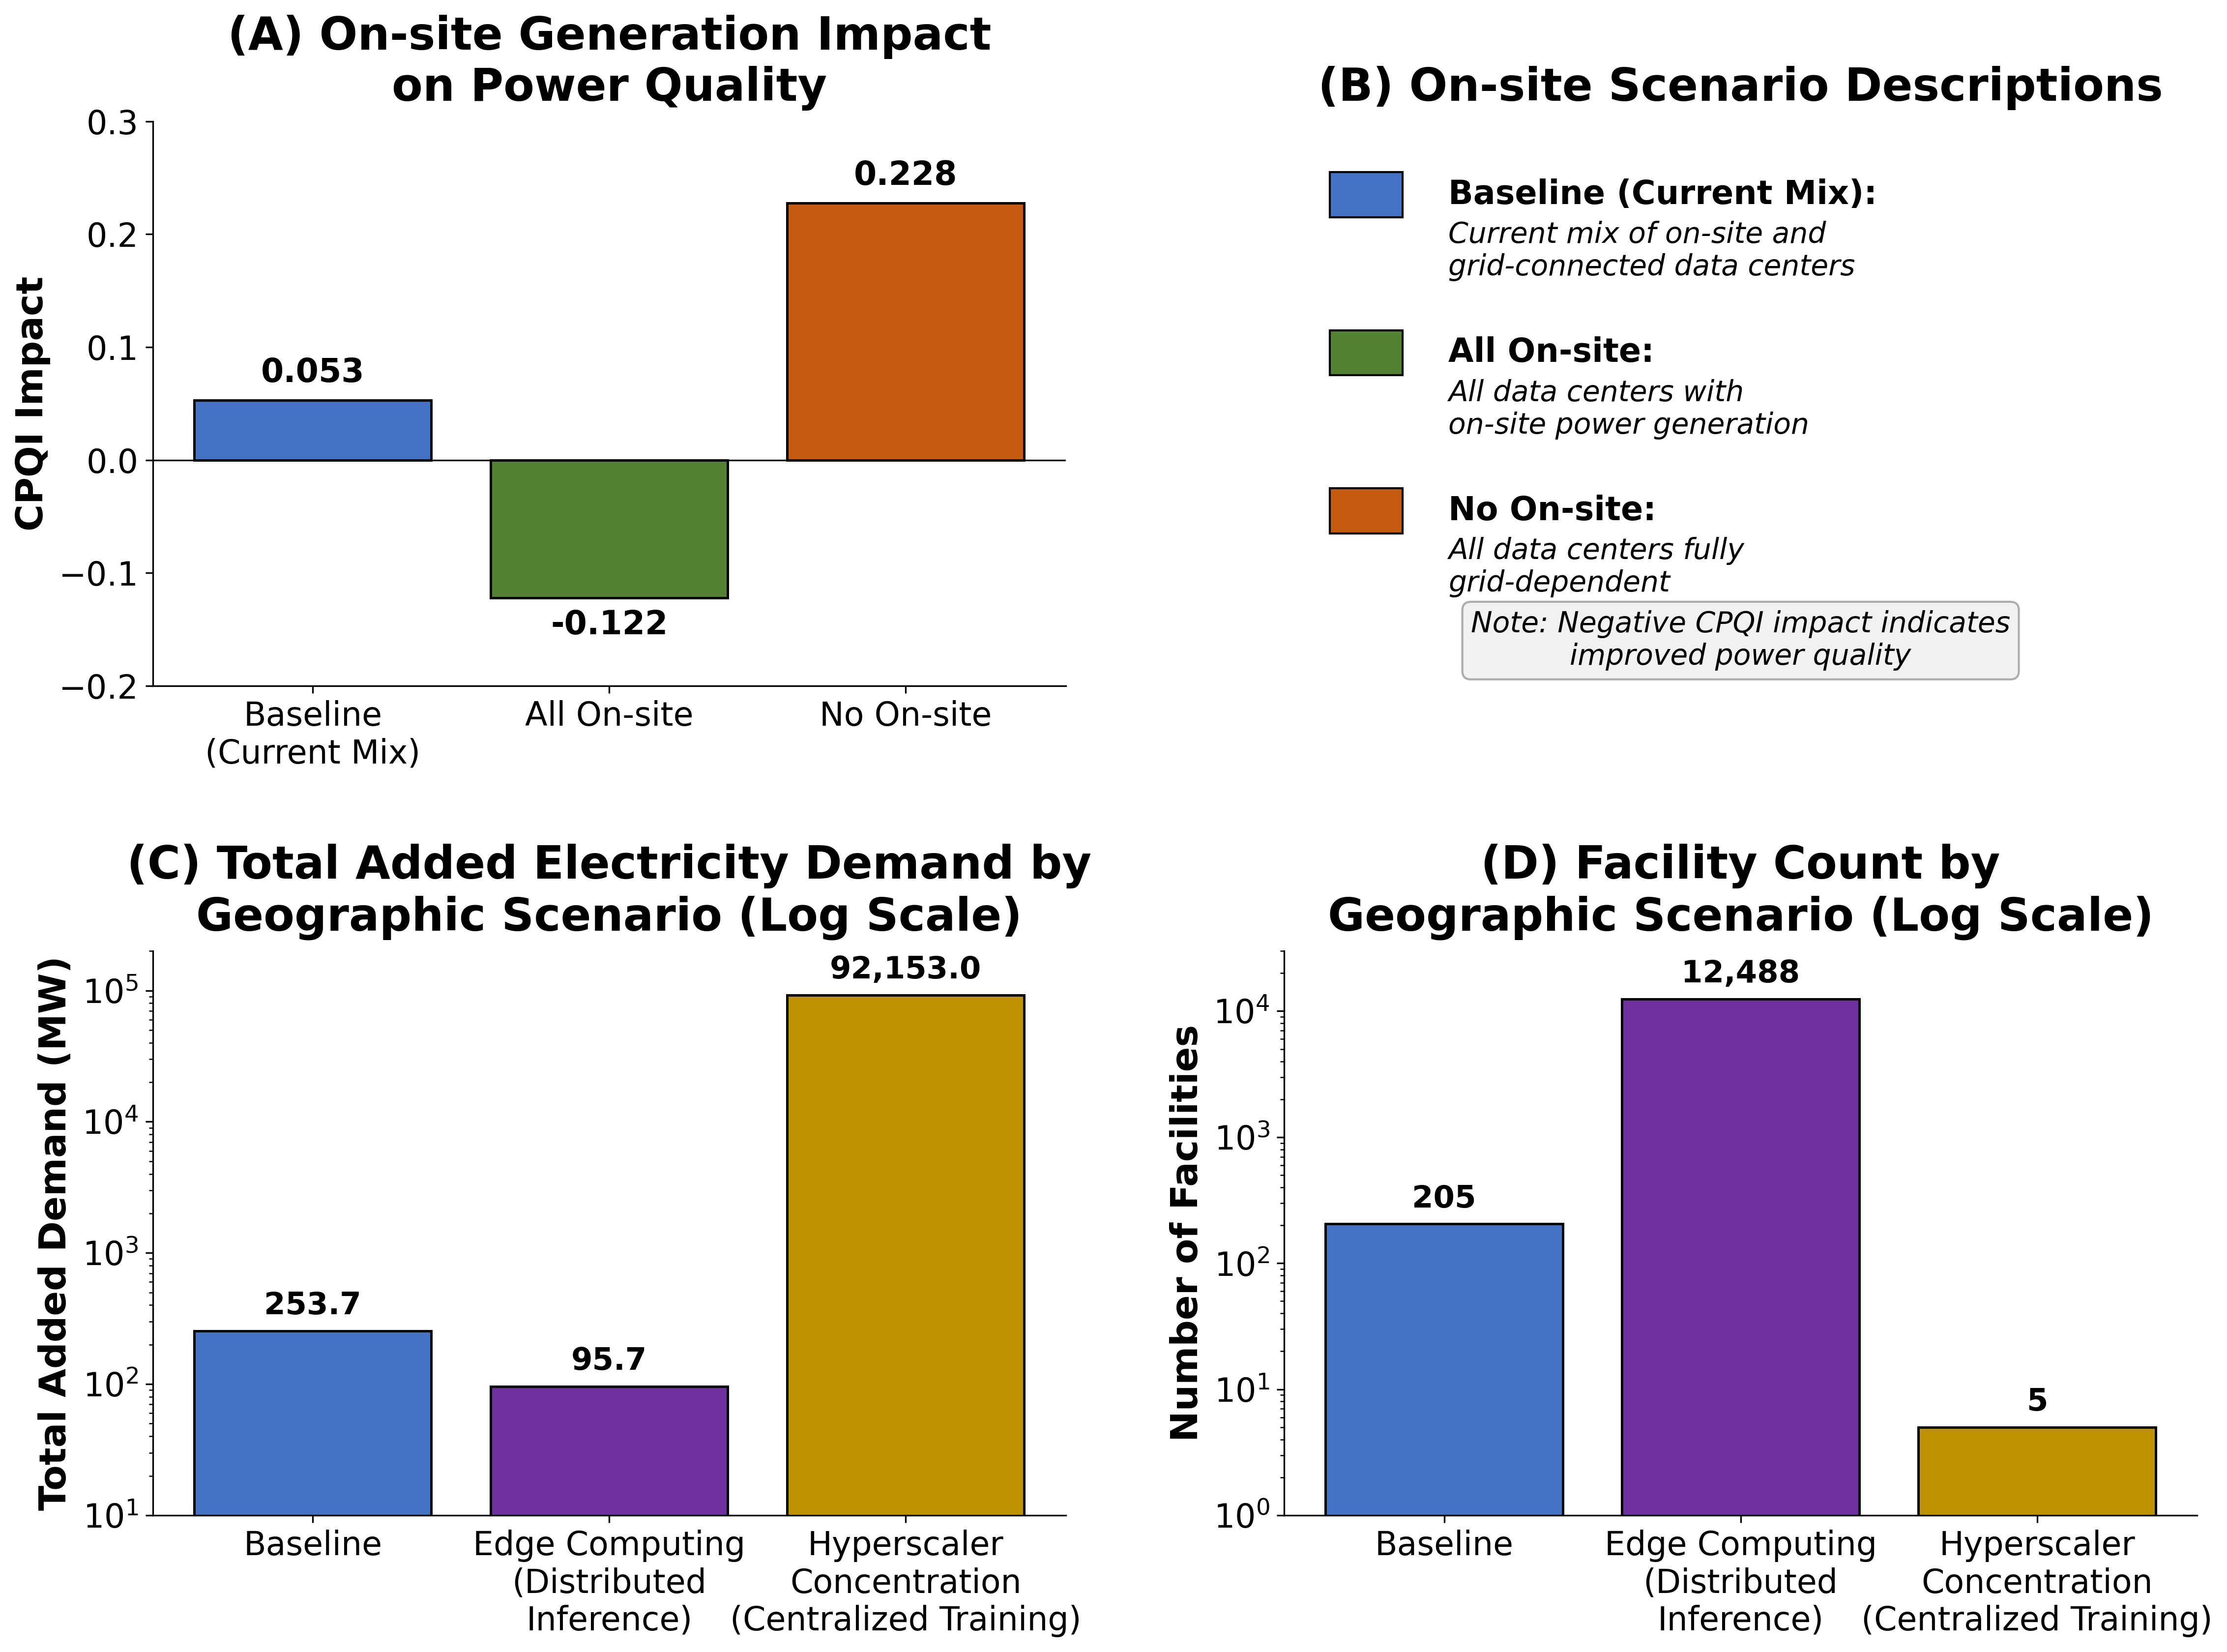
\includegraphics[width=.9\linewidth]{Figures/combined_analysis_figure.png}
    \caption{Effects of Geographic Concentration and On-site Generation on AI Impacts on the grid.}
    \label{fig:CounterfactualCombined}
    \vspace{-2em}
\end{figure}

% \subsubsection{Behind-the-Meter Power Generation Scenarios}

% One major question about the evolution of AI infrastructure concerns the role of on-site generation for data centers. To date, on-site generation investments have been relatively limited, but many investments are planned. On-site generation has numerous benefits due to the data center need for continuous direct current power with fast interconnection times and a non-smooth load profile. Significant investments in behind-the-meter power can benefit both the grid and the companies making the investments.

% We consider both a world where behind-the-meter power becomes standard and a world where on-site generation plays no role in data center power. Figure~\ref{fig:btm_scenarios} demonstrates how baseline AI impacts would change under these scenarios. Remarkably, considering only treated observations, universal adoption of BTM power would shift the impact of data centers from a net detriment to power quality to a net improvement. This suggests that data center investment in power generation substantially improves overall grid outcomes.


% \subsubsection{Additional Counterfactuals}

% Other counterfactuals could be performed with our framework, including:
% \begin{itemize}
%     \item Regressing inference coefficients on reported model queries to determine the scaling effect of additional queries on demand.
%     \item Estimating carbon emissions impacts based on the generation mix in affected regions.
%     \item Analyzing how time-of-use pricing or demand response programs might alter the temporal distribution of AI loads and associated grid impacts.
% \end{itemize}
% These extensions are left for future work.

\section{Conclusion}\label{sec:conclusion_aipower}

This paper provides the first causal estimates of how AI-driven data center demand affects U.S.\ electricity markets. Exploiting the staggered release of frontier large language models as natural experiments, we find that AI workloads cause statistically and economically significant deterioration in power quality, increase fossil fuel generation on the order of hundreds of GWh, and raise wholesale electricity prices by up to 25\% in heavily treated zones. These effects are consistent with the predictions of our game-theoretic model of hyperscaler electricity procurement, which formalizes the \emph{timing wedge}---the temporal mismatch between when data centers consume electricity and when their contracted or credited renewable generation produces.

The economic implications are substantial. The timing wedge means that the voluntary procurement instruments favored by hyperscalers---renewable energy certificates and power purchase agreements---do not internalize the externalities they are designed to address. RECs, as financial transfers unbundled from physical dispatch, leave real-time fossil generation and grid stress unaffected. PPAs improve on this margin only modestly absent firming or storage. Our counterfactual analyses reinforce this finding: universal adoption of on-site generation would reverse the sign of power quality effects, transforming data centers from a net grid liability into a net contributor. This result suggests that the externality is not inherent to AI demand per se, but rather to the spatial and temporal misalignment between that demand and clean generation---a misalignment that current market instruments fail to correct.

These findings speak directly to ongoing policy debates over renewable energy procurement design. Proposals for hourly matching, such as the 24/7 Carbon-Free Energy framework, attempt to close the timing wedge by requiring temporal alignment of clean energy credits with consumption. Our model provides a framework for evaluating such proposals: tightening matching granularity raises the effective price of RECs in high-carbon hours, increases the private value of storage, and induces entry of temporally aligned generation. The empirical heterogeneity we document between data centers with and without on-site generation offers suggestive evidence that policies promoting behind-the-meter investment could yield grid-wide benefits. Geographic redistribution of inference workloads---toward edge computing or toward high-supply, low-load regions---offers an additional policy lever, though with important tradeoffs between transmission costs and local reliability.

Our analysis has limitations. The parallel trends assumption underpinning any difference-in-differences design may be violated if treated and control regions were already diverging prior to model releases, or if generators anticipated these releases. Spillovers across interconnected regions and heterogeneous effects by grid topology or model type may attenuate or bias our estimates. Our power quality dataset, while novel, covers a limited time horizon that constrains our ability to characterize long-run trends. Finally, frontier model releases are an imperfect proxy for the continuous evolution of AI compute demand, and the mapping from a discrete release event to actual deployment and load is necessarily noisy.

Despite these limitations, the results carry clear implications for electricity market design. As AI workloads grow, regulators and system operators will need instruments that address not only the volume but the temporal and spatial profile of incremental demand. Our findings suggest that annual renewable accounting provides insufficient incentive for the investments in storage, on-site generation, and demand flexibility that would align private procurement with system-level reliability and emissions goals. The methodological approach developed here---combining econometric causal identification with publicly available grid data---is portable to other settings where proprietary operational data are unavailable, including the effects of AI on network congestion, cooling water demand, or semiconductor supply chains.

\bibliographystyle{cas-model2-names}
\bibliography{Energy}

\appendix
\section{Appendix}
\subsection{Results Tables}

\begin{table}[hbp]
\centering
\caption{Estimated Impact of AI Model Releases on Power Quality}
\label{tab:AIModelsPowerQuality}
\small
\begin{tabular}{l l r r r}
\toprule
Model & Provider & Coefficient & Std. Error & $R^{2}$ \\
\midrule
GPT-4.5                  & Microsoft   & 0.327*** & 0.087 & 0.327 \\
Llama 4 Behemoth (preview) & Facebook  & 0.325*** & 0.074 & 0.313 \\
Claude 3 Opus            & Google      & 0.278*** & 0.043 & 0.462 \\
Gemini 1.5 Pro           & Google      & 0.223*** & 0.026 & 0.451 \\
GPT-4o                   & Microsoft   & 0.198*** & 0.044 & 0.331 \\
GPT-4                    & Microsoft   & 0.176*** & 0.033 & 0.408 \\
Claude 3.7 Sonnet        & Google      & 0.161*** & 0.041 & 0.357 \\
Chinchilla               & Google      & 0.143*** & 0.038 & 0.570 \\
PaLM (540B)              & Google      & 0.142*** & 0.029 & 0.587 \\
LaMDA                    & Google      & 0.134**  & 0.044 & 0.564 \\
PaLM 2                   & Google      & 0.133*** & 0.024 & 0.465 \\
Claude 3.5 Sonnet        & Google      & 0.126*** & 0.036 & 0.378 \\
OPT-175B                 & Facebook    & 0.104*** & 0.023 & 0.467 \\
Gemini 1.0 Ultra         & Google      & 0.103*** & 0.021 & 0.409 \\
Llama 3.1-405B           & Facebook    & 0.052    & 0.034 & 0.315 \\
Minerva (540B)           & Google      & 0.031    & 0.023 & 0.519 \\
Parti                    & Google      & 0.031    & 0.023 & 0.519 \\
GPT-4 Turbo              & Microsoft   & 0.030*   & 0.017 & 0.308 \\
GPT-3.5                  & Microsoft   & -0.049** & 0.018 & 0.390 \\
Flan-PaLM 540B           & Google      & -0.051*  & 0.026 & 0.508 \\
U-PaLM (540B)            & Google      & -0.051*  & 0.026 & 0.508 \\
Amazon Titan             & Amazon AWS  & -0.086***& 0.016 & 0.380 \\
\bottomrule
\end{tabular}
\begin{flushleft}
\footnotesize
Notes: Robust standard errors in parentheses. Significance levels: *** $p<0.01$, ** $p<0.05$, * $p<0.1$.
\end{flushleft}
\end{table}

\begin{table}[htbp]\centering
\caption{Difference-in-Differences Estimates of Data Center Announcements on Cumulative Total Queue Capacity (MW)}
\begin{threeparttable}
\begin{tabular}{lcc}
\toprule
& (1) & (2) \\
& No FE & County \& Year FE \\
\midrule
Post Announcement & 714.459\sym{**} & 150.741\sym{*} \\
& (293.890) & (87.001) \\
Intercept & 366.406\sym{***} & -188.142\sym{***} \\
& (19.361) & (13.395) \\
\midrule
Observations & 128,700 & 128,700 \\
R$^2$ & 0.010 & 0.780 \\
Adj.\ R$^2$ & 0.010 & 0.777 \\
Fixed Effects & No & County \& Year \\
\bottomrule
\end{tabular}
\begin{tablenotes}[flushleft]
\footnotesize
\item Cluster-robust standard errors in parentheses. 
\item \sym{*} $p<0.10$, \sym{**} $p<0.05$, \sym{***} $p<0.01$. 
\end{tablenotes}
\end{threeparttable}
\label{DIDTotal}
\end{table}

\begin{table}[htbp]\centering
\caption{Difference-in-Differences Estimates of Data Center Announcements on Cumulative Gas Queue Capacity (MW)}
\begin{threeparttable}
\begin{tabular}{lcc}
\toprule
& (1) & (2) \\
& No FE & County \& Year FE \\
\midrule
Post $\times$ Announced Capacity & 0.324\sym{***} & 0.250\sym{**} \\
& (0.105) & (0.117) \\
Intercept & 175.718\sym{***} & -43.457\sym{***} \\
& (18.388) & (13.229) \\
\midrule
Observations & 16,380 & 16,380 \\
R$^2$ & 0.012 & 0.610 \\
Adj.\ R$^2$ & 0.012 & 0.604 \\
Fixed Effects & No & County \& Year \\
\bottomrule
\end{tabular}
\begin{tablenotes}[flushleft]
\footnotesize
\item Cluster-robust standard errors in parentheses. 
\item \sym{*} $p<0.10$, \sym{**} $p<0.05$, \sym{***} $p<0.01$. 
\end{tablenotes}
\end{threeparttable}
\label{DIDGas}
\end{table}

\begin{table}[htbp]\centering
\caption{Difference-in-Differences Estimates of Data Center Announcements on Cumulative Gas Queue Capacity (MW), No Interaction}
\begin{threeparttable}
\begin{tabular}{lcc}
\toprule
& (1) & (2) \\
& No FE & County \& Year FE \\
\midrule
Post Announcement & 98.976 & 273.893\sym{***} \\
& (68.413) & (79.284) \\
Intercept & 176.560\sym{***} & 63.585\sym{***} \\
& (18.656) & (1.28e-11) \\
\midrule
Observations & 16,380 & 16,380 \\
R$^2$ & 0.003 & 0.522 \\
Adj.\ R$^2$ & 0.002 & 0.514 \\
Fixed Effects & No & County \& Year \\
\bottomrule
\end{tabular}
\begin{tablenotes}[flushleft]
\footnotesize
\item Cluster-robust standard errors in parentheses. 
\item \sym{*} $p<0.10$, \sym{**} $p<0.05$, \sym{***} $p<0.01$. 
\end{tablenotes}
\end{threeparttable}
\label{DIDNGInteract}
\end{table}

% POST-TREATMENT EFFECTS
\begin{table}[htbp]
\centering
\caption{Post-Treatment: Estimated Impact of AI Model Releases on Aggregate Electricity Demand}
\label{tab:ai_demand_post}
\resizebox{\columnwidth}{!}{%
\begin{threeparttable}
\begin{tabular}{l l r r r r}
\toprule
Model & Provider & Coefficient & $p$-value & $R^{2}$ & Aggregate Impact (MWh) \\
\midrule
Switch                         & Google     & 124.46 & $<0.001$ & 0.628 & 4,154,379 \\
DALL\text{-}E                  & Microsoft  &  81.54 & $<0.001$ & 0.627 & 2,910,208 \\
GPT\text{-}3.5                 & Microsoft  &  76.08 & $<0.001$  & 0.622 & 1,034,517 \\
mT5\text{-}XXL                 & Google     &  63.48 & $<0.001$              & 0.625 &   420,630 \\
Megatron\text{-}Turing NLG 530B& Microsoft &  46.15 & $<0.001$  & 0.628 & 1,692,209 \\
Codex                          & Microsoft  &  35.60 & 0.0211                & 0.630 & 2,132,043 \\
Minerva (540B)                 & Google     &  24.03 & 0.4305                & 0.624 & 1,372,621 \\
Parti                          & Google     &  20.14 & 0.4692                & 0.625 & 1,183,787 \\
Flan\text{-}PaLM (540B)        & Google     &  17.36 & 0.0501                & 0.622 &   504,750 \\
U\text{-}PaLM (540B)           & Google     &  17.36 & 0.0501                & 0.622 &   504,750 \\
OPT\text{-}175B                & Facebook   &  12.85 & 0.0161                & 0.624 &   583,999 \\
ByT5\text{-}XXL                & Google     &   1.28 & 0.9584                & 0.624 &    66,424 \\
ProtT5\text{-}XXL              & Google     &  -1.42 & 0.9370                & 0.629 &   -64,268 \\
Meta Pseudo Labels             & Google     &  -3.996& 0.8284                & 0.628 &  -118,203 \\
FLAN 137B                      & Google     &  -4.97 & 0.7971                & 0.624 &  -167,480 \\
Chinchilla                     & Google     & -23.54 & 0.0980                & 0.628 &  -834,056 \\
PaLM (540B)                    & Google     & -24.53 & 0.0714                & 0.628 &  -873,641 \\
LaMDA                          & Google     & -27.41 & 0.1362                & 0.626 &  -643,963 \\
GLaM                           & Google     & -27.76 & 0.3485                & 0.625 &  -750,319 \\
Gopher (280B)                  & Google     & -30.32 & 0.3113                & 0.625 &  -813,756 \\
\bottomrule
\end{tabular}
\begin{tablenotes}
\item Notes: Coefficients and p-values are taken from \texttt{post\_coefficient} and \texttt{post\_p\_value}. Aggregate impact uses \texttt{post\_aggregate\_demand\_increase}. The headline causal claim of the chapter is the pooled stacked-DiD coefficient reported in Table~\ref{tab:combined_results}; the model-by-model rows above are reported as \emph{descriptive} per-event estimates rather than as confirmatory tests, since each row identifies off a single release event with limited statistical power. The sign pattern is consistent with the scaling story discussed in Section~\ref{sec:counterfactuals}: smaller and earlier-generation models (Chinchilla, PaLM 540B, LaMDA, Gopher 280B) carry small or negative point estimates with wide confidence bands, while larger and later-generation models (GPT-4.5, Llama 4 Behemoth, Claude 3 Opus) carry substantially larger and more precisely estimated positive coefficients. We do not interpret negative point estimates on individual older or smaller models as evidence against the AI-induced demand effect.
\end{tablenotes}
\end{threeparttable}}
\label{PostTreatment}
\end{table}

% PRE-TREATMENT EFFECTS
\begin{table}[htbp]
\centering
\caption{Pre-Treatment: Estimated Impact of AI Model Releases on Aggregate Electricity Demand}
\label{tab:ai_demand_pre}
\resizebox{\columnwidth}{!}{%
\begin{threeparttable}
\begin{tabular}{l l r r r r}
\toprule
Model & Provider & Coefficient & $p$-value & $R^{2}$ & Aggregate Impact (MWh) \\
\midrule
Switch                         & Google     &  89.77 & $<0.001$ & 0.628 &   268,851 \\
DALL\text{-}E                  & Microsoft  &  66.90 & $<0.001$ & 0.627 &    43,755 \\
GPT\text{-}3.5                 & Microsoft  &  39.60 & $<0.001$             & 0.622 & 1,501,640 \\
% mT5\text{-}XXL                 & Google     &   —    & —                    & 0.625 &      —    \\
Megatron\text{-}Turing NLG 530B& Microsoft &  35.96 & 0.0138               & 0.628 & 2,088,496 \\
Codex                          & Microsoft  &  28.63 & 0.0108               & 0.630 & 1,245,855 \\
Minerva (540B)                 & Google     & -22.51 & 0.0972               & 0.624 &  -781,775 \\
Parti                          & Google     & -22.94 & 0.1056               & 0.625 &  -734,906 \\
Flan\text{-}PaLM (540B)        & Google     &  29.16 & 0.3543               & 0.622 & 1,475,972 \\
U\text{-}PaLM (540B)           & Google     &  29.16 & 0.3543               & 0.622 & 1,475,972 \\
OPT\text{-}175B                & Facebook   & -21.77 & 0.2825               & 0.624 &  -502,990 \\
ByT5\text{-}XXL                & Google     &  -6.20 & 0.7410               & 0.624 &  -177,165 \\
ProtT5\text{-}XXL              & Google     & 101.54 & $<0.001$ & 0.629 & 3,280,303 \\
Meta Pseudo Labels             & Google     & 168.29 & $<0.001$& 0.628 & 4,122,856 \\
FLAN 137B                      & Google     &   3.41 & 0.8961               & 0.624 &    181,878 \\
Chinchilla                     & Google     & -23.61 & 0.4060               & 0.628 &  -583,230 \\
PaLM (540B)                    & Google     & -22.84 & 0.4174               & 0.628 &  -554,841 \\
LaMDA                          & Google     & -27.80 & 0.3750               & 0.626 &  -817,029 \\
GLaM                           & Google     & -12.52 & 0.4856               & 0.625 &  -413,053 \\
Gopher (280B)                  & Google     &  -8.12 & 0.6566               & 0.625 &  -271,852 \\
\bottomrule
\end{tabular}
\begin{tablenotes}
\item Notes: Coefficients and p-values are taken from \texttt{pre\_coefficient} and \texttt{pre\_p\_value}. Aggregate impact uses \texttt{pre\_aggregate\_demand\_increase}. Dashes indicate missing values in the spreadsheet. As with Table~\ref{PostTreatment}, model-by-model rows are presented as \emph{descriptive} per-event estimates rather than confirmatory tests; the chapter's identifying inference comes from the pooled stacked-DiD specification.
\end{tablenotes}
\end{threeparttable}}
\label{PreTreatment}
\end{table}

\newpage

\subsection{Expanded Dataset Description}

Below, maps can be found providing more detail on the dataset alongside tables on the datasets and the dataset sample selection criteria.

\begin{figure}[h]
    \centering
    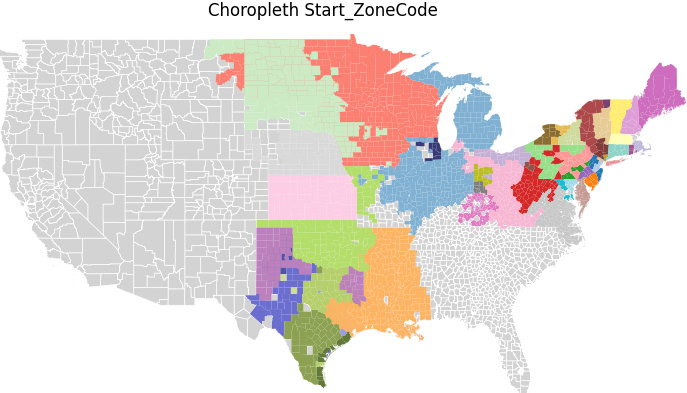
\includegraphics[width=\linewidth]{Figures/ZoneMap (1).png}
    \caption{Map of zones for demand model.}
    \label{fig:placeholder}
\end{figure}

\begin{figure}[h]
    \centering
    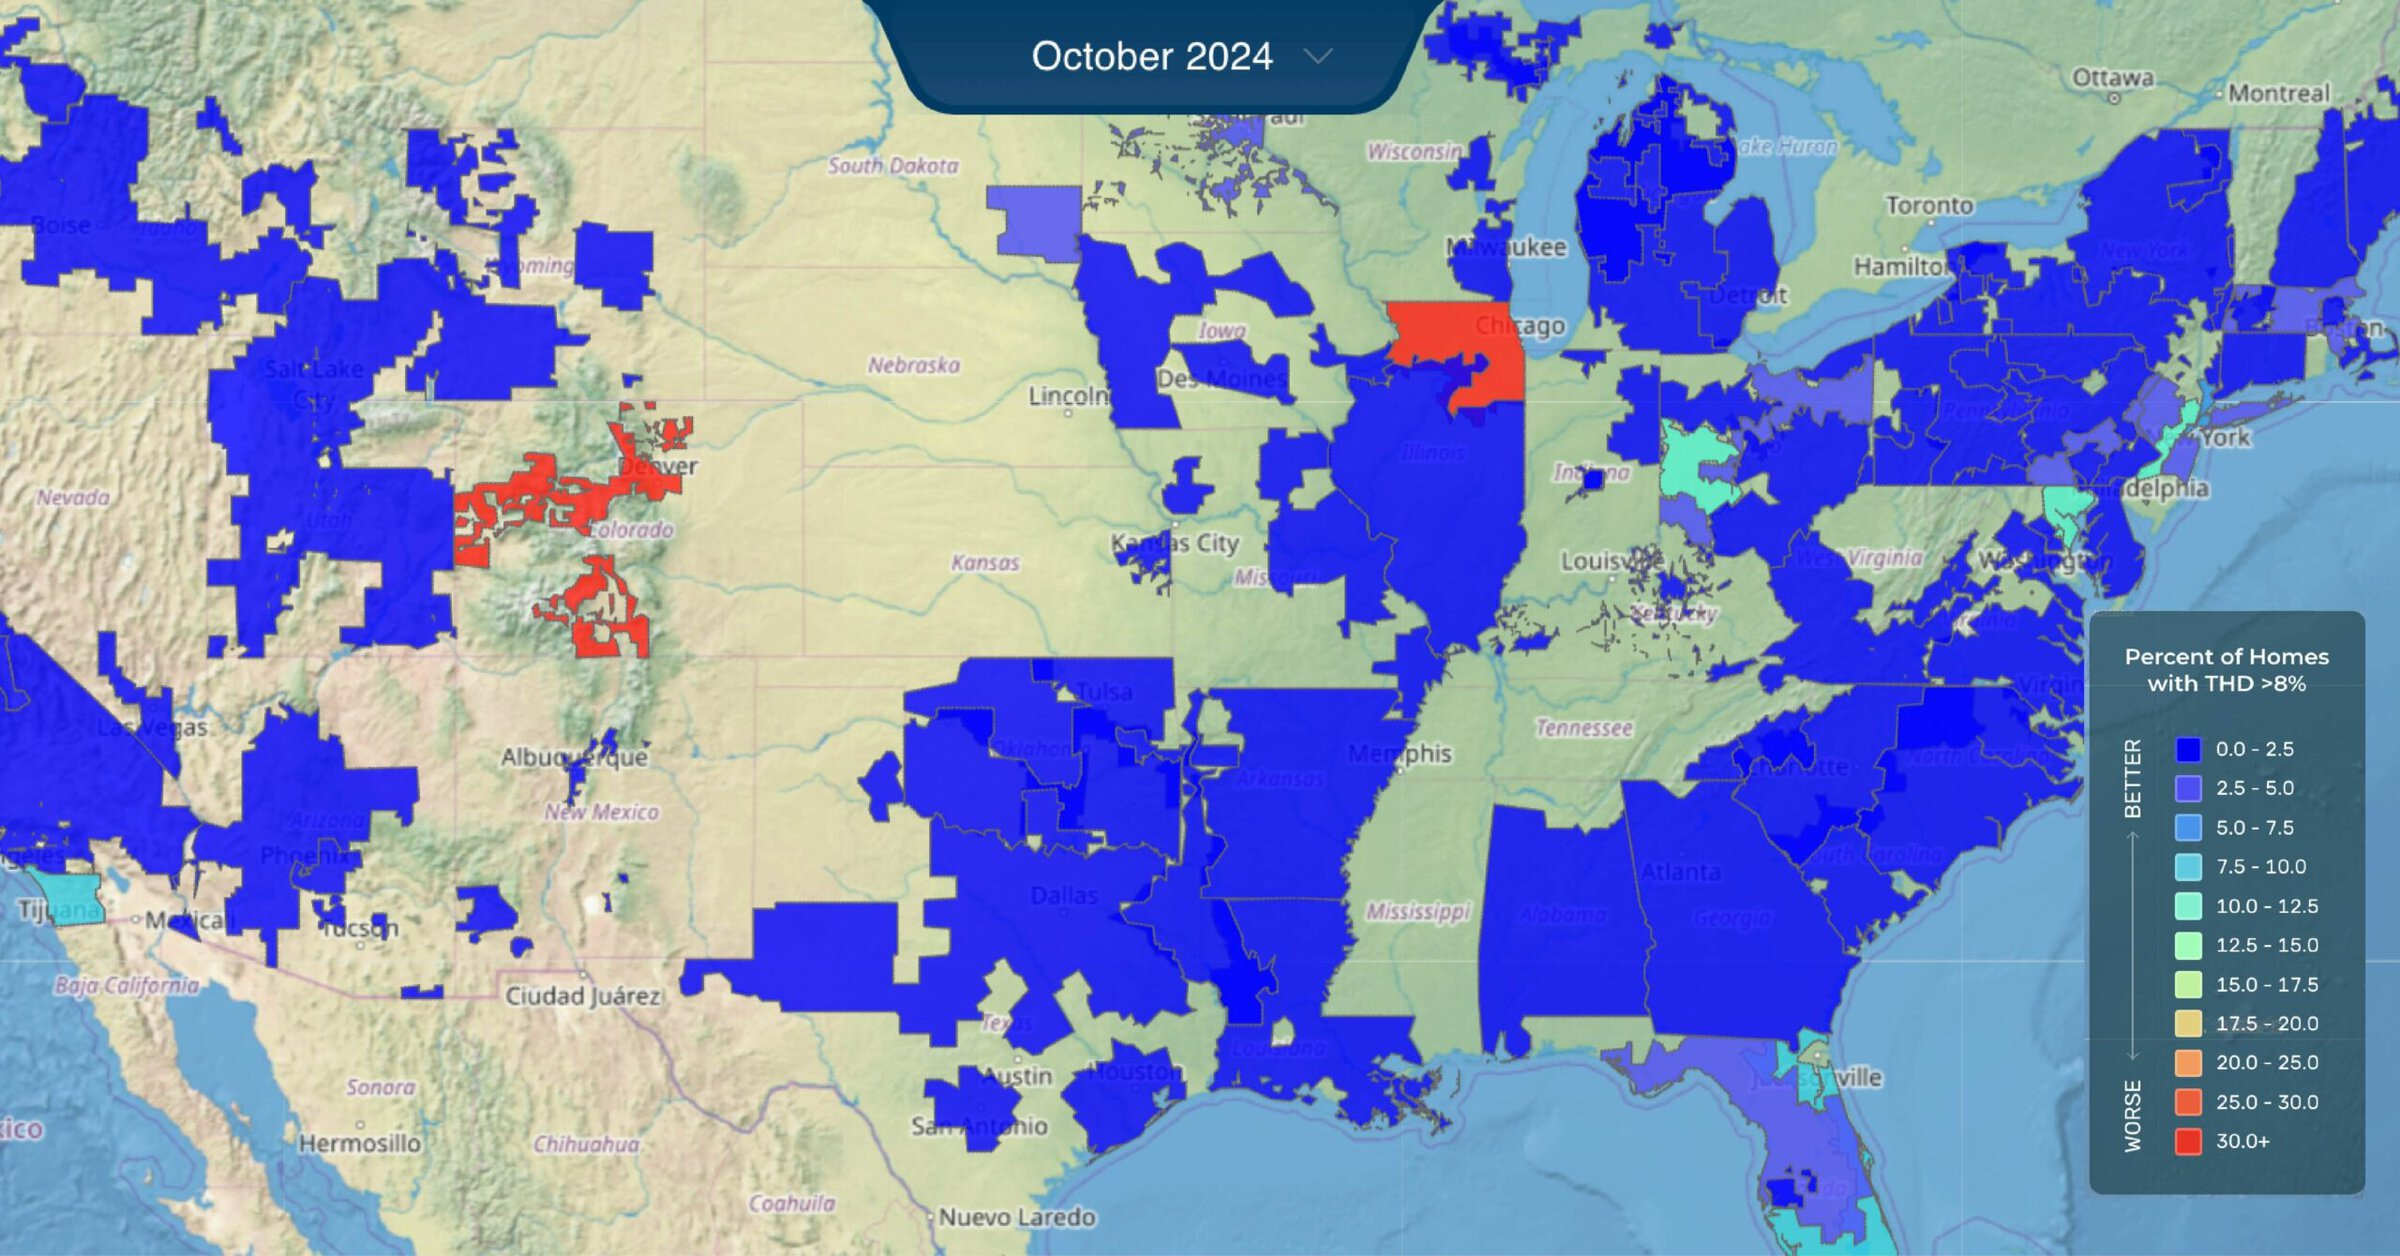
\includegraphics[width=\linewidth]{Figures/THD Dataset.jpg}
    \caption{Map of Retail Electric Utilities for Whisker Labs Data.}
    \label{fig:placeholder}
\end{figure}

\begin{figure}
    \centering
    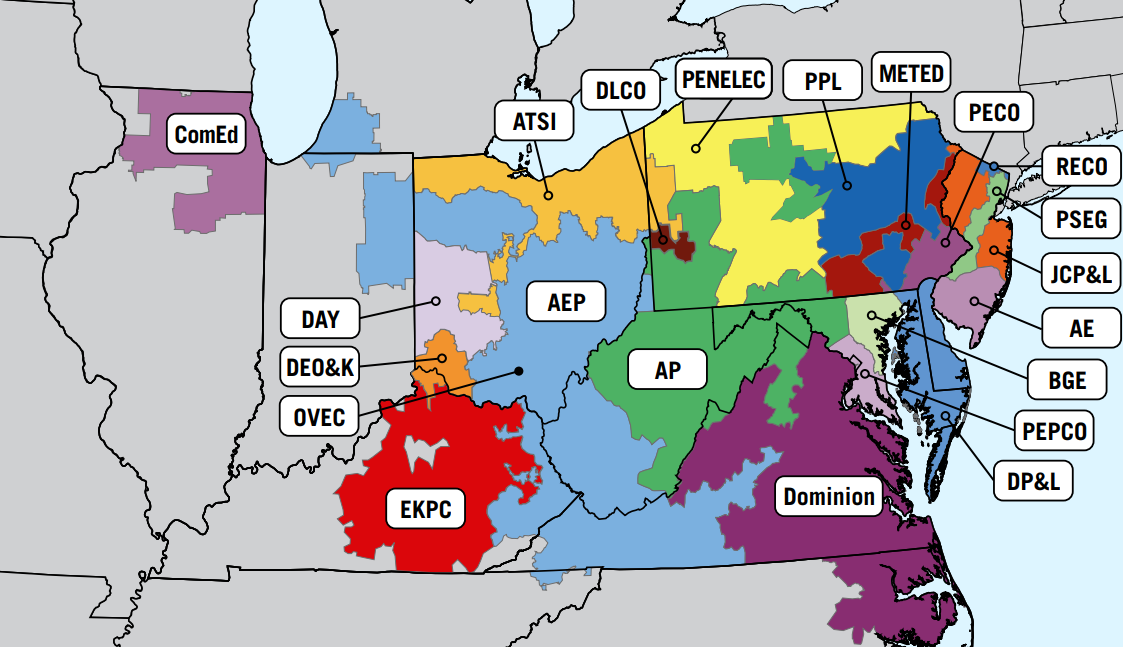
\includegraphics[width=0.75\linewidth]{Figures/PJMZonalMap.png}
    \caption{Map of PJM by Zones.}
    \label{fig:placeholder}
\end{figure}


\clearpage
\begin{sidewaystable}[p]
\centering
\caption{Expanded description of data sources (for appendix).}
\label{tab:DataSourcesExpanded}

\begin{adjustbox}{max width=\textheight} % <-- key: rotated page's usable width
\begin{threeparttable}
\begin{tabular}{p{0.18\textheight} p{0.55\textheight} p{0.25\textheight}}
\toprule
\textbf{Source} & \textbf{Content and Granularity} & \textbf{Use in Analysis} \\
\midrule
\multicolumn{3}{c}{\textbf{Q1: Difference-in-Differences (Power Quality)}} \\
\midrule
Aterio & Data center locations, establishment/expansion/retirement dates, ownership, and operational capacity (MW). Data are available at the facility level and updated annually. & Defines treatment regions; links AI model releases to hyperscaler-owned centers. \\
Whisker Labs & Consumer Power Quality Index (CPQI, composite measure of surges, sags, brownouts, interruptions) and Total Harmonic Distortion (THD, waveform distortion). Provided at county level, hourly frequency. & Outcome variables for DiD regressions. \\
Meteostat & Hourly temperature and precipitation, aggregated at the county level. Coverage includes all U.S. counties with weather stations. & Controls for demand fluctuations and renewable generation variability. \\
ISOs & Geographic boundary shapefiles and wholesale price data at zonal level. Boundaries digitized from ISO-provided maps; prices available hourly. & Market alignment and regional controls. \\
EIA & Retail service territory shapefiles, at utility level, updated periodically. & Used to define treatment/control boundaries and reconcile geographies. \\
\midrule
\multicolumn{3}{c}{\textbf{Q2: Instrumental Variables (Fossil Demand)}} \\
\midrule
EPA CAMPD & Hourly generator-level demand (MWh) and unit-specific heat rates (Btu/kWh). Coverage 2021--2023. & Generator demand is outcome; heat rates serve as instruments for prices. \\
S\&P Capital IQ & Daily natural gas price series, Henry Hub benchmark. National coverage. & Instrument for price and fuel-cost control. \\
Aterio & Generator proximity to data centers owned by releasing companies, matched at 20-mile radius. & Defines treatment generators in IV design. \\
Meteostat & Hourly temperature and precipitation, as above. & Controls for demand and renewable variability. \\
ISOs & Wholesale price series, zonal level, hourly frequency. & Market-level controls. \\
\midrule
\multicolumn{3}{c}{\textbf{Q3: Counterfactual Analyses (Scaling, Efficiency,  \& Tech Development)}} \\
\midrule
Whisker Labs & CPQI and THD (as above). Used to establish baseline deterioration in power quality. & Benchmark outcomes for scaling projections. \\
Epoch & AI model metadata: release dates, FLOPs, parameter counts. Public dataset with model-level detail. & Used for scaling regressions and efficiency counterfactuals. \\
GPU Experiments & Energy use measured on NVIDIA A6000 GPUs. Experiments run with batch size 4, sequence length 1024, and 200 inferences. Each bar in results represents total energy; lighter portion indicates communication overhead. Data collected in-house on 8xA6000 cluster. & Provides empirical GPU energy baselines for counterfactual scaling exercises. \\
\bottomrule
\end{tabular}
\end{threeparttable}
\end{adjustbox}
\end{sidewaystable}
\clearpage

\newpage
\clearpage

% 1. These two lines force the sidewaystable to center vertically on the page
\setlength{\rotFPtop}{0pt plus 1fil}
\setlength{\rotFPbot}{0pt plus 1fil}

\begin{sidewaystable}[p] % [p] forces it to be on its own page
\centering
\setlength{\tabcolsep}{3pt}
\renewcommand{\arraystretch}{0.95}

\caption{Dataset sample selection and summary statistics}
\label{tab:SampleSelection}

\begin{threeparttable}
\footnotesize
% 2. Use \linewidth so it fills the text block, but relies on margins for centering
\begin{tabularx}{\linewidth}{lXl} 
\toprule
\textbf{Dataset} & \textbf{Content / Summary Statistics} & \textbf{Sample Selection} \\
\midrule
Aterio & Data center locations, ownership, and capacity; mapped to ISO zones, EIA service territories, and counties & Hyperscaler data centers (Meta, Microsoft, Amazon, Google; Anthropic via Google) \\
\midrule
Whisker Labs & Reliability measures: CPQI ($N=2{,}683$, mean=0.52, s.d.=0.42); THD (mean=1.81, s.d.=6.77) & 72 retail electric utilities, monthly data 2022--2025 \\
\midrule
CAMPD & Generator-level demand: mean 218 MW (s.d.=158); operating times $\approx 1$ & Several thousand fossil generators, hourly data 2021--2023 \\
\midrule
ISOs & Wholesale electricity prices: mean $\$51$/MWh (s.d.=148); zonal boundaries & Deregulated markets in Eastern Interconnection and ERCOT \\
\midrule
Weather (Meteostat) & Temperature (mean=17°C, s.d.=11.4); precipitation (mean=0.12 mm, s.d.=0.91) & Matched by county/zone, hourly or daily resolution \\
\midrule
External Controls & Natural gas prices, ISO market data, geography/time harmonization & Used for both DiD and IV regressions \\
\bottomrule
\end{tabularx}

\begin{tablenotes}
\scriptsize
\item Notes: Time series are harmonized at hourly or monthly resolution depending on source. Unified panel supports both difference-in-differences (power quality) and instrumental variable (demand) regressions. Maps of sample regions provided in the appendix.
\end{tablenotes}
\end{threeparttable}

\end{sidewaystable}
\clearpage
\newpage

\subsection{Dataset Creation Diagram}

\begin{figure}[htbp]
\centering
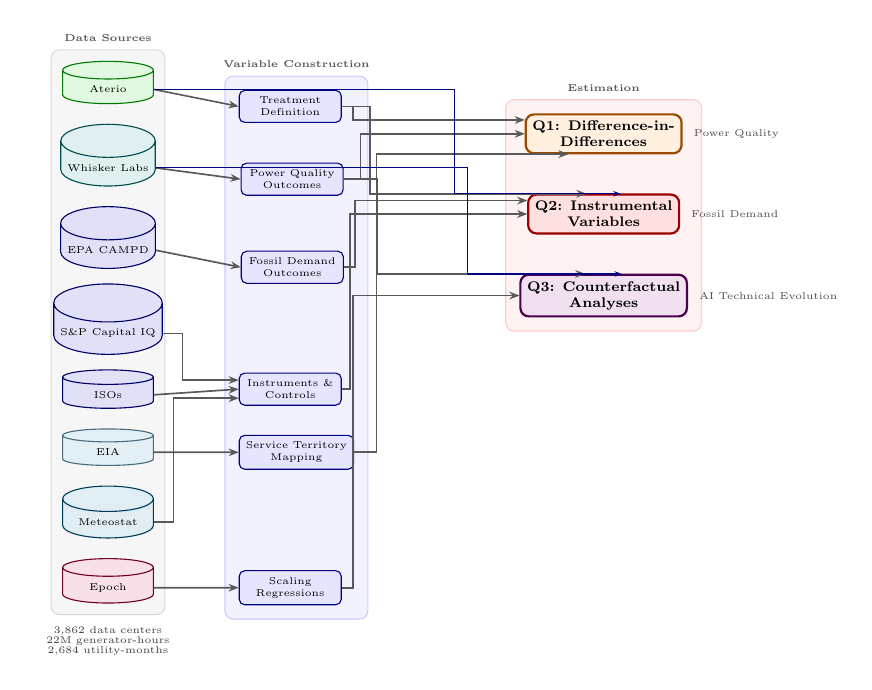
\begin{tikzpicture}[
    scale=0.72,
    transform shape,
    node distance=0.48cm and 0.7cm,
    % === STYLES ===
    source/.style={
        cylinder,
        shape border rotate=90,
        draw=#1!60!black,
        fill=#1!12,
        text centered,
        minimum height=1.55em,
        minimum width=1.6cm,
        aspect=0.35,
        font=\tiny,
        align=center
    },
    source/.default=green,
    process/.style={
        rectangle,
        draw=blue!50!black,
        fill=blue!10,
        text centered,
        rounded corners=2pt,
        minimum height=1.35em,
        minimum width=1.8cm,
        font=\tiny,
        align=center
    },
    model/.style={
        rectangle,
        draw=#1!60!black,
        fill=#1!12,
        thick,
        text centered,
        rounded corners=3pt,
        minimum height=1.85em,
        minimum width=2.4cm,
        font=\scriptsize\bfseries,
        align=center
    },
    model/.default=red,
    arrow/.style={
        -{Stealth[scale=0.65]},
        semithick,
        color=gray!70!black
    },
    directarrow/.style={
        -{Stealth[scale=0.55]},
        color=blue!50!black,
        thin
    },
    grouplabel/.style={
        font=\tiny\bfseries,
        color=gray!70!black
    },
    annot/.style={
        font=\scriptsize,
        color=gray!60!black
    }
]

% === COLUMN 1: DATA SOURCES ===

% AI/Data Center Data (green shades)
\node[source=green!80!black] (aterio) {Aterio};

% Power Quality Data (teal shades)
\node[source=teal, below=0.35cm of aterio] (whisker) {Whisker Labs};

% Generator/Market Data (blue shades)
\node[source=blue!70!black, below=0.35cm of whisker] (campd) {EPA CAMPD};
\node[source=blue!70!black, below=0.26cm of campd] (spiq) {S\&P Capital IQ};
\node[source=blue!70!black, below=0.26cm of spiq] (isos) {ISOs};

% Government/Geographic (cyan shades)
\node[source=cyan!70!black, below=0.35cm of isos] (eia) {EIA};

% Weather (blue-green shades)
\node[source=blue!60!green, below=0.35cm of eia] (weather) {Meteostat};

% AI Model Data (purple shades)
\node[source=purple, below=0.35cm of weather] (epoch) {Epoch};

% === COLUMN 2: DATA CONSTRUCTION STEPS ===

% Treatment Definition
\node[process, right=1.5cm of aterio, yshift=-0.3cm] (treat_def) {Treatment\\Definition};

% Outcome Construction
\node[process, right=1.5cm of whisker, yshift=-0.2cm] (outcome_pq) {Power Quality\\Outcomes};

% Fossil Demand Construction
\node[process, right=1.5cm of campd, yshift=-0.3cm] (fossil_dem) {Fossil Demand\\Outcomes};

% Instrument Construction
\node[process, right=1.5cm of isos, yshift=0.1cm] (instruments) {Instruments \&\\Controls};

% Service Territory Mapping
\node[process, right=1.5cm of eia] (territory) {Service Territory\\Mapping};

% Scaling Data
\node[process, right=1.5cm of epoch] (scaling) {Scaling\\Regressions};

% === COLUMN 3: ANALYSIS MODELS ===

% Q1: DiD Model
\node[model=orange, right=3.2cm of outcome_pq, yshift=0.8cm] (q1) {Q1: Difference-in-\\Differences};

% Q2: IV Model  
\node[model=red, below=0.7cm of q1] (q2) {Q2: Instrumental\\Variables};

% Q3: Counterfactual Model
\node[model=violet, below=0.7cm of q2] (q3) {Q3: Counterfactual\\Analyses};

% === CONNECTIONS ===

% To Treatment Definition
\draw[arrow] (aterio.east) -- (treat_def.west);

% To Power Quality Outcomes
\draw[arrow] (whisker.east) -- (outcome_pq.west);

% To Fossil Demand Outcomes
\draw[arrow] (campd.east) -- (fossil_dem.west);

% To Instruments & Controls
\draw[arrow] (spiq.east) -- ++(0.35,0) |- (instruments.170);
\draw[arrow] (isos.east) -- (instruments.west);
\draw[arrow] (weather.east) -- ++(0.35,0) |- (instruments.190);

% To Service Territory Mapping
\draw[arrow] (eia.east) -- (territory.west);

% To Scaling Regressions
\draw[arrow] (epoch.east) -- (scaling.west);

% === CONNECTIONS TO MODELS ===

% Q1 connections
\draw[arrow] (treat_def.east) -- ++(0.2,0) |- (q1.170);
\draw[arrow] (outcome_pq.east) -- ++(0.3,0) |- (q1.west);
\draw[arrow] (territory.east) -- ++(0.4,0) |- (q1.210);

% Q2 connections
\draw[arrow] (treat_def.east) -- ++(0.5,0) |- (q2.130);
\draw[arrow] (fossil_dem.east) -- ++(0.2,0) |- (q2.170);
\draw[arrow] (instruments.east) -- ++(0.15,0) |- (q2.west);

% Q3 connections
\draw[arrow] (outcome_pq.east) -- ++(0.6,0) |- (q3.130);
\draw[arrow] (scaling.east) -- ++(0.2,0) |- (q3.west);

% Direct data feeds
\draw[directarrow] (aterio.east) -- ++(5.3,0) |- (q2.50);
\draw[directarrow] (whisker.east) -- ++(5.5,0) |- (q3.50);

% === BACKGROUND GROUPINGS ===
\begin{scope}[on background layer]
    % Raw Data Sources
    \node[fit=(aterio)(epoch), 
          fill=gray!7, 
          rounded corners=3pt, 
          draw=gray!30,
          inner sep=4pt] (rawbox) {};
    \node[grouplabel, above=0.02cm of rawbox.north] {Data Sources};
    
    % Data Construction
    \node[fit=(treat_def)(scaling)(territory)(instruments), 
          fill=blue!5, 
          rounded corners=3pt, 
          draw=blue!20,
          inner sep=5pt] (constructbox) {};
    \node[grouplabel, above=0.02cm of constructbox.north] {Variable Construction};
    
    % Models
    \node[fit=(q1)(q2)(q3), 
          fill=red!5, 
          rounded corners=3pt, 
          draw=red!20,
          inner sep=5pt] (modelbox) {};
    \node[grouplabel, above=0.02cm of modelbox.north] {Estimation};
\end{scope}

% === ANNOTATIONS ===
% Observation counts
\node[font=\fontsize{4}{5}\selectfont, color=gray!50!black, below=0.08cm of rawbox.south, text width=2.6cm, align=center] 
    {3,862 data centers\\22M generator-hours\\2,684 utility-months};

% Model annotations
\node[annot, right=0.08cm of q1.east] {\tiny Power Quality};
\node[annot, right=0.08cm of q2.east] {\tiny Fossil Demand};
\node[annot, right=0.08cm of q3.east] {\tiny AI Technical Evolution};

\end{tikzpicture}
\caption{Data sources and analysis pipeline. Data sources flow through variable construction into three estimation strategies addressing power quality impacts (Q1), fossil fuel demand (Q2), and counterfactual scaling scenarios (Q3).}
\label{fig:DataDiagram}
\end{figure}

\subsection{Construction of Zonal Geographic Maps}\label{zonalMappingEfforts}


A central requirement of the analysis is the ability to match generators to geographic areas in a manner consistent with ISO market structure while preserving as much spatial detail as possible. Because publicly available GIS shapefiles for ISO-defined market zones are incomplete, inconsistent, or entirely unavailable, the construction of zonal maps required substantial manual effort. I view this process as a significant contribution of the paper.

The guiding principle throughout was to aggregate only where necessary to permit consistent geographic matching and econometric analysis, while keeping the data at the lowest feasible spatial resolution. In all cases, zonal boundaries were explicitly restricted to lie within ISO boundaries using GIS shapefiles defining Independent System Operator footprints. This prevents generators, loads, or weather observations from being incorrectly assigned across ISOs.

\paragraph{General Approach.}
The mapping procedure proceeds in three steps. First, ISO boundaries are imposed as a hard geographic constraint. Second, ISO-specific zones are mapped to counties or county aggregates using a combination of published documentation, utility maps, and GIS overlays. Third, generators are assigned to zones using EIA Form 860 identifiers where available, and county-level geographic matching otherwise. Hand-constructed crosswalk tables are used to reconcile inconsistent geographic schemas across datasets.

Where counties do not align cleanly with ISO zones, counties are split proportionally based on geographic overlap and engineering judgment, applied consistently across datasets.

\paragraph{ERCOT.}
For ERCOT, zones are based primarily on the system’s published weather zones, which in most cases map cleanly to county boundaries. Where weather zones do not align perfectly with counties, I split counties across zones using GIS overlays to preserve contiguity and proportional area. Several ERCOT datasets rely on alternative geographic schemas (e.g., hub- or region-based reporting); in these cases, I construct hand-built mapping tables to reconcile these schemas with the zonal structure used in the analysis.

\paragraph{PJM.}
PJM required the most extensive manual mapping effort. PJM publishes a large number of zones, many of which do not correspond cleanly to county boundaries. I manually mapped each PJM zone to counties using a combination of PJM documentation, utility service maps, and GIS inspection. In cases where counties span multiple PJM zones, judgment was applied to split counties as cleanly as possible while preserving geographic continuity. Where appropriate for the analysis, zones were subsequently aggregated into regions to support the distribution of generation data.

\paragraph{SPP.}
SPP zones were mapped using a similar procedure, combining transmission zone definitions with county-level utility maps and GIS shapefiles. In several states, publicly available utility maps with county labels were used to guide assignments. As with PJM, counties were split only where necessary, and always within ISO boundaries.

\paragraph{NYISO.}
For NYISO, zones were mapped based on reliability assessment zones using a zonal county map. These zones align relatively well with county boundaries, allowing for a clean assignment in most cases.

\paragraph{MISO.}
MISO presents a comparatively clean case: all zonal boundaries correspond to state-level regions. As a result, counties were assigned directly to MISO zones based on state boundaries, eliminating the need for county splitting.

\paragraph{ISO New England.}
ISO New England zones are primarily defined at the state level, with the notable exception of Massachusetts, which is divided into three wholesale zones. For Massachusetts, I manually mapped counties to zones using GIS overlays and ISO documentation, splitting counties where necessary to maintain geographic consistency.

\paragraph{Generator Assignment.}
Generators are assigned to zones using ISO labels from EIA Form 860 wherever possible, which minimizes the risk of misassignment across ISOs. When ISO labels are unavailable or insufficiently granular, generators are matched using county-level geographic information derived from plant location data. This layered approach ensures consistency between generator assignment, zonal geography, and ISO market structure.

Overall, this mapping procedure enables the construction of consistent zonal maps that balance geographic precision with analytical tractability, forming the backbone of the spatial analysis in the paper.

\subsection{Counterfactual}
Figure \ref{fig:counterQuality} shows the power quality line we fit for performing counterfactuals.

\begin{figure}[h]
    \centering
    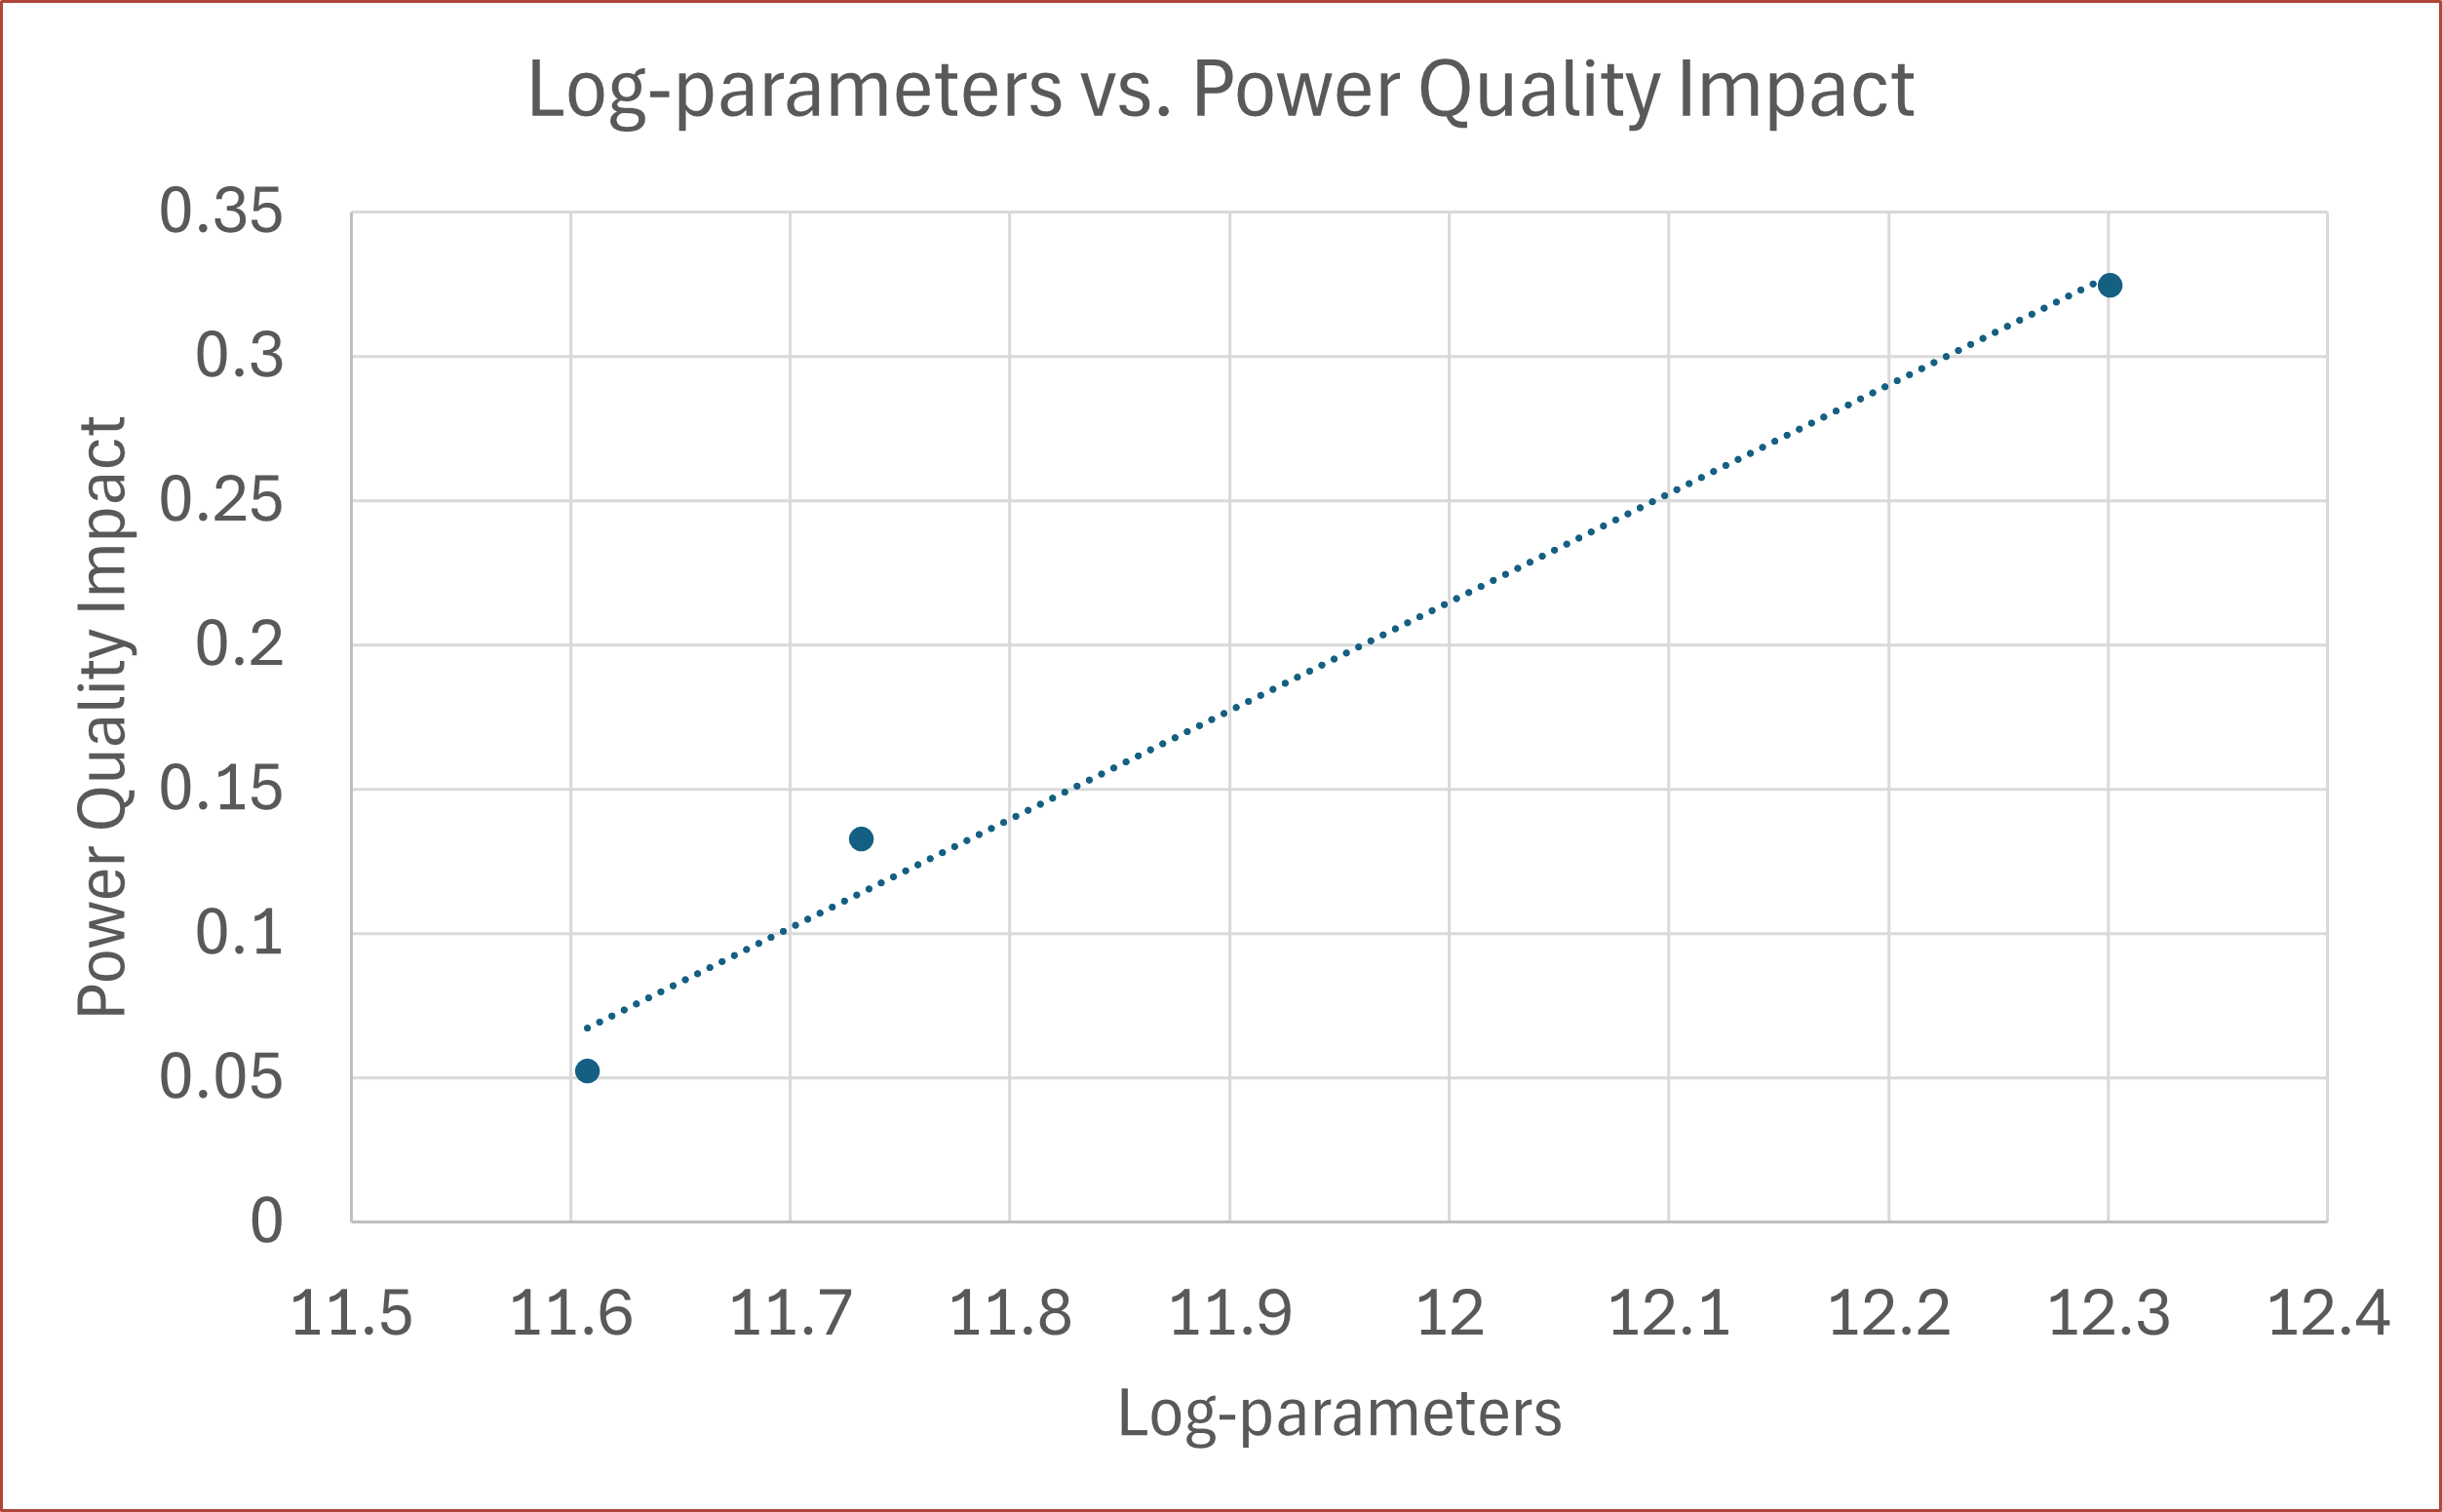
\includegraphics[width=0.5\linewidth]{Figures/Power Quality Impact1.png}
    \caption{Power Quality Impact for Counterfactuals.}
    \label{fig:counterQuality}
\end{figure}

\subsection{Calculation of Comparisons}

We calculate the household average energy usage based on data provided by \cite{USHouseholdConsumption}. We simply divide our estimates by the provided numbers to get the number of households for our comparisons.

\subsection{Code and Replication}
\label{appendix:replication}

This appendix provides comprehensive documentation for replicating the empirical analysis. All code and data processing scripts are available in the supplementary materials.

\subsubsection{Software Requirements}
\label{appendix:software}

The analysis pipeline is implemented in Python 3.11 and designed to execute on a Linux HPC cluster using the SLURM workload manager. Scripts include environment-aware path detection to support local execution on Windows systems.

\paragraph{Computational Resources.} The full pipeline requires approximately 32GB of memory and 8 CPU cores, with an expected runtime of 12--24 hours on an HPC cluster (24--48 hours for local execution). Memory-intensive operations include spatial joins for utility service territory matching and construction of stacked difference-in-differences datasets.

\paragraph{Python Dependencies.} The analysis requires the following packages: \texttt{pandas} ($\geq$2.0), \texttt{numpy} ($\geq$1.24), \texttt{scipy} ($\geq$1.10), \texttt{statsmodels} ($\geq$0.14), \texttt{linearmodels} ($\geq$5.0), \texttt{geopandas} ($\geq$0.14), \texttt{shapely} ($\geq$2.0), \texttt{fiona} ($\geq$1.9), \texttt{pyproj} ($\geq$3.6), \texttt{rtree} ($\geq$1.0), \texttt{geopy} ($\geq$2.3), \texttt{gdal} ($\geq$3.6), \texttt{matplotlib} ($\geq$3.7), and \texttt{seaborn} ($\geq$0.12). We use \texttt{micromamba} for environment management on the cluster.

\subsubsection{Data Sources}
\label{appendix:data}

Table~\ref{tab:data_sources} summarizes the primary data sources used in the analysis. All data files should be placed in a \texttt{Data/} subdirectory relative to the code directory.

\begin{table}[htbp]
\centering
\caption{Data Sources and Descriptions}
\label{tab:data_sources}
\footnotesize % Reduces font size slightly to fit narrow columns
% @{} removes extra side padding to maximize space
% >{\raggedright\arraybackslash}X wraps text and left-aligns it
\begin{tabularx}{\columnwidth}{@{} >{\raggedright\arraybackslash}X >{\raggedright\arraybackslash}X l @{}}
\toprule
\textbf{File} & \textbf{Description} & \textbf{Source} \\
\midrule
\multicolumn{3}{l}{\textit{Electricity Demand Analysis}} \\
\texttt{EPAData.csv} & Hourly emissions and generation & EPA CAMPD \\
\texttt{epa\_eia\_crosswalk.csv} & EPA--EIA facility identifiers & Custom \\
\texttt{data\_center\_inventory.csv} & Data center locations with AI flags & Aterio \\
\texttt{mapData.shp} & Zone boundary shapefiles & FERC/ISO \\
\texttt{TransmissionPriceLoad.csv} & Zonal electricity prices and load & ISO/RTO \\
\texttt{ExtendedNGPriceData.csv} & Natural gas price time series & EIA \\
\texttt{mapDatawithWeather.csv} & Zone-level weather data & NOAA \\
\midrule
\multicolumn{3}{l}{\textit{Power Quality Analysis}} \\
% Manually broke this long filename to ensure it fits the column
\texttt{electric-retail-service- \newline territories.shp} & Utility service area boundaries & EIA-861 \\
\texttt{Epoch Database - Notable Models.csv} & AI model release dates & Epoch AI \\
\texttt{PowerQuality.csv} & Customer Power Quality Index & Whisker Labs \\
\texttt{THD.csv} & Total Harmonic Distortion & PQ Monitor \\
\midrule
\multicolumn{3}{l}{\textit{Robustness Checks}} \\
\texttt{ai\_model\_dates\_verified.csv} & Verified API release dates & Manual \\
\bottomrule
\end{tabularx}
\end{table}

\subsubsection{Pipeline Architecture}
\label{appendix:pipeline}

The analysis executes in four sequential phases, with internal parallelization within phases. Figure~\ref{fig:pipeline} illustrates the data flow.

\paragraph{Phase 1: Data Construction.} The script \texttt{CreateDataIVDiffinDiffCAMPD.py} constructs the panel dataset by merging EPA emissions data with data center locations, electricity market data, and natural gas prices. Key variables created include: \texttt{treated} (binary indicator for zones within proximity of AI data centers), \texttt{post} (binary indicator for post-AI-model-release periods), and \texttt{treatment\_intensity} (continuous measure based on model compute requirements). Output: \texttt{panelIVDiDData.csv}.

\paragraph{Phase 2: Main Regressions.} Four scripts execute in parallel:
\begin{enumerate}[noitemsep,topsep=0pt]
    \item \texttt{IVDiffinDiffCAMPD.py}: IV-DiD estimation for electricity demand using two-stage least squares with natural gas prices as instruments and zone/month fixed effects.
    \item \texttt{IVDiffinDiffCAMPD\_Stacked.py}: Stacked DiD methodology following \citet{cengiz2019effect} to address heterogeneous treatment timing, with unit-by-event and time-by-event fixed effects.
    \item \texttt{DiffinDiff.py}: Difference-in-differences for power quality outcomes (CPQI and THD) at the utility level.
    \item \texttt{DiffinDiff\_Stacked.py}: Stacked DiD for power quality, addressing staggered treatment timing across AI model releases.
\end{enumerate}

\paragraph{Phase 3: Robustness and Visualization.} Two parallel jobs: (i) \texttt{IVDiffinDiff\_VerifiedDates.py} re-estimates the main specifications using hand-verified API release and training completion dates rather than publication dates; (ii) \texttt{IVDiffinDiff\_SupplyElasticity\_PJM.py} estimates supply-side responses followed by \texttt{AI\_Price\_Impact\_Choropleth\_PJM.py} for visualization.

\paragraph{Phase 4: Counterfactual Analysis.} The script \texttt{CounterfactualAnalysis.py} performs policy counterfactuals including efficiency gain scenarios (10\%, 20\%, 30\%, 40\% improvements), channel shutdown scenarios (training-only versus inference-only operations), geographic redistribution (edge computing versus hyperscaler concentration), and on-site expansion/contraction scenarios.

\begin{figure}[htbp]
\centering
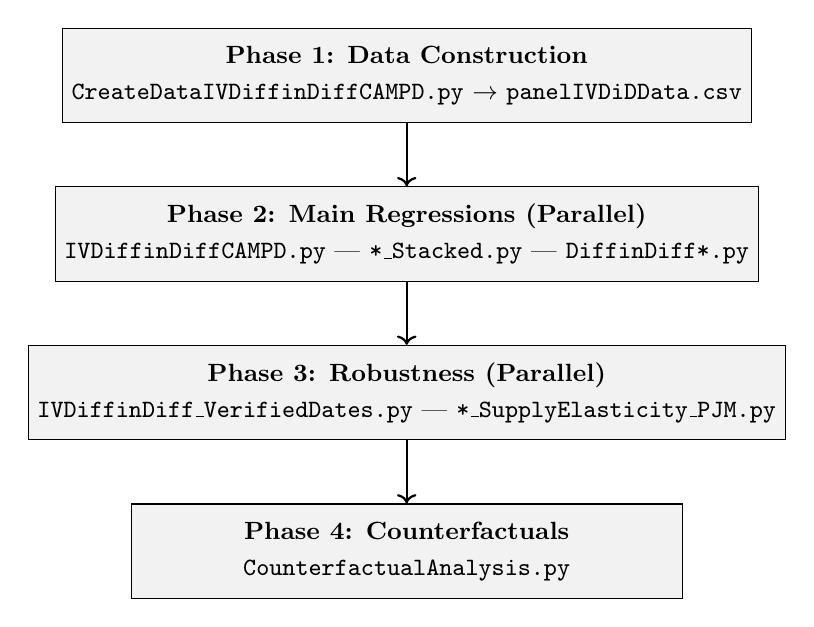
\begin{tikzpicture}[
    node distance=0.8cm,
    phase/.style={rectangle, draw, fill=gray!10, minimum width=7cm, minimum height=1.2cm, align=center, font=\small},
    script/.style={rectangle, draw, fill=white, minimum width=3cm, minimum height=0.7cm, align=center, font=\scriptsize},
    arrow/.style={->, thick}
]
% Phase 1
\node[phase] (p1) {\textbf{Phase 1: Data Construction}\\[2pt]\texttt{CreateDataIVDiffinDiffCAMPD.py} $\rightarrow$ \texttt{panelIVDiDData.csv}};

% Phase 2
\node[phase, below=of p1] (p2) {\textbf{Phase 2: Main Regressions (Parallel)}\\[2pt]\texttt{IVDiffinDiffCAMPD.py} | \texttt{*\_Stacked.py} | \texttt{DiffinDiff*.py}};

% Phase 3
\node[phase, below=of p2] (p3) {\textbf{Phase 3: Robustness (Parallel)}\\[2pt]\texttt{IVDiffinDiff\_VerifiedDates.py} | \texttt{*\_SupplyElasticity\_PJM.py}};

% Phase 4
\node[phase, below=of p3] (p4) {\textbf{Phase 4: Counterfactuals}\\[2pt]\texttt{CounterfactualAnalysis.py}};

% Arrows
\draw[arrow] (p1) -- (p2);
\draw[arrow] (p2) -- (p3);
\draw[arrow] (p3) -- (p4);
\end{tikzpicture}
\caption{Analysis Pipeline Architecture}
\label{fig:pipeline}
\end{figure}

\subsubsection{Key Estimation Parameters}
\label{appendix:parameters}

The main specifications use the following default parameters, which can be modified for robustness checks:

\begin{itemize}[noitemsep,topsep=0pt]
    \item Proximity threshold: 20 miles (for defining treatment based on data center locations)
    \item Fixed effects: Zone and month
    \item Stacked DiD event windows: $\pm$2 months (default), with robustness checks at $\pm$1, $\pm$3, and $\pm$6 months
    \item Instruments: Natural gas prices (exogenous cost shifter for electricity supply)
\end{itemize}

\subsubsection{Executing the Analysis}
\label{appendix:execution}

\paragraph{HPC Cluster (SLURM).} Submit the job file with \texttt{sbatch Full\_Analysis\_Pipeline.job}. Monitor progress with \texttt{squeue -u \$USER} and check phase-specific logs in \texttt{logs/phase*/}.

\paragraph{Local Execution.} Scripts automatically detect local execution and adjust file paths accordingly. Run Phase 1 first, then Phases 2--3 scripts can execute in parallel, followed by Phase 4:
\begin{verbatim}
python CreateDataIVDiffinDiffCAMPD.py          # Phase 1
python IVDiffinDiffCAMPD.py &                  # Phase 2 (parallel)
python DiffinDiff.py &
wait
python CounterfactualAnalysis.py               # Phase 4
\end{verbatim}

\subsubsection{Output Files}
\label{appendix:outputs}

Table~\ref{tab:outputs} summarizes the primary output files generated by the pipeline.

\begin{table}[htbp]
\centering
\caption{Primary Output Files}
\label{tab:outputs}
\footnotesize % Essential for fitting long filenames in narrow columns
\begin{tabularx}{\columnwidth}{@{} >{\raggedright\arraybackslash}X >{\raggedright\arraybackslash}X @{}}
\toprule
\textbf{File/Directory} & \textbf{Description} \\
\midrule
\texttt{panelIVDiDData.csv} & Constructed panel dataset \\
\texttt{IVDiffinDiffResults.csv} & IV-DiD demand coefficients and standard errors \\
\texttt{DiffinDiffResults.csv} & CPQI regression results \\
\texttt{THD\_DiffinDiffResults.csv} & THD regression results \\
% Manual breaks are required for long paths in narrow columns
\texttt{stacked\_did\_iv\_ \newline results/} & Stacked DiD coefficients and plots (demand) \\
\texttt{stacked\_did\_cpqi\_ \newline results/} & Stacked DiD coefficients and plots (CPQI) \\
\texttt{stacked\_did\_thd\_ \newline results/} & Stacked DiD coefficients and plots (THD) \\
\texttt{IVDiffinDiff\_Verified \newline Dates\_Results.csv} & Robustness with verified dates \\
\texttt{pjm\_ai\_supply\_impact\_ \newline by\_zone.csv} & PJM zone-level supply impacts \\
\texttt{counterfactual\_ \newline outputs/} & Scenario analysis results and visualizations \\
\bottomrule
\end{tabularx}
\end{table}

\subsubsection{Shared Module}
\label{appendix:shared}

The stacked DiD methodology is implemented in a shared module (\texttt{StackedDiD.py}) used by both the demand and power quality analyses. Key functions include: \texttt{create\_stacked\_dataset()} for constructing mini-datasets for each treatment event; \texttt{run\_stacked\_did\_regression()} for executing stacked DiD regressions with appropriate fixed effects; \texttt{aggregate\_treatment\_effects()} for cohort-weighted aggregation of treatment effects; and \texttt{plot\_event\_study()} for visualization of event-time coefficients. This modular design ensures methodological consistency across outcome variables.

\subsubsection{Reproducibility Notes}
\label{appendix:reproducibility}

Several implementation details enhance reproducibility. First, scripts automatically handle multicollinearity via \texttt{check\_and\_fix\_multicollinearity()} functions that detect and address near-singular matrices in the fixed effects specifications. Second, memory-intensive operations include explicit garbage collection (\texttt{gc.collect()}) to manage memory on systems with limited resources. Third, all random seeds are fixed where applicable to ensure deterministic results. Fourth, the SLURM job file specifies exact resource requirements (32GB memory, 8 CPUs across 4 tasks) that can be scaled based on available infrastructure. Log files in \texttt{logs/phase*/} provide detailed execution traces for debugging.

\subsection{Specifically Verified Models}

\begin{table}[htbp]
\centering
\caption{Documented Training Locations}
\label{tab:training_locations}
\begin{tabular}{@{}llllll@{}}
\toprule
Model & Provider & Location & Confirmation & Primary Source & Citation \\
\midrule
GPT-4 & OpenAI & West Des Moines, Iowa & Confirmed & Brad Smith (May 2023) & \cite{smith2023iowa} \\
PaLM, LaMDA, MUM & Google & Mayes County, Oklahoma & Confirmed & Google Cloud Blog (Apr 2023) & \cite{googlecloud2023mlhub} \\
BLOOM & BigScience & Orsay, France (Jean Zay) & Confirmed & Hugging Face model card & \cite{luccioni2022bloom} \\
Llama 1-2 & Meta & RSC (location unconfirmed) & Partial & Meta model card & \cite{hpcwire2023rsc} \\
Gemini Ultra & Google & Multiple sites (unspecified) & Partial & Thomas Kurian interview & \cite{kurian2023dcd} \\
Claude models & Anthropic & AWS/Google Cloud (regions) & Partial & Anthropic announcements & \cite{anthropic2025infrastructure} \\
Megatron-Turing NLG & NVIDIA/Microsoft & Santa Clara area (Selene) & Confirmed & NVIDIA/Microsoft blogs & \cite{nvidia2021megatron} \\
\bottomrule
\end{tabular}
\end{table}

\begin{longtable}{p{2.2cm} p{3.4cm} p{3.0cm} p{2.3cm} p{1.6cm} p{2.0cm}}
\caption{Verified Model Dates}
\label{tab:verified_model_dates}\\
\toprule
Company & Model & Date Type & Date & Precision & Source \\
\midrule
\endfirsthead

\toprule
Company & Model & Date Type & Date & Precision & Source \\
\midrule
\endhead

\bottomrule
\endfoot

OpenAI & GPT-3 & API Release & 2020-06-11 & day & \cite{openai_api_2020} \\
OpenAI & GPT-3 & API Release & 2021-11-18 & day & \cite{openai_api_nowaitlist_2021} \\
OpenAI & Codex & API Release & 2021-08-10 & day & \cite{openai_codex_2021} \\
OpenAI & DALL-E 2 & API Release & 2022-11-03 & day & \cite{openai_dalle_api_beta_2022} \\
OpenAI & ChatGPT & API Release & 2022-11-30 & day & \cite{openai_chatgpt_2022} \\
OpenAI & GPT-3.5-turbo & API Release & 2023-03-01 & day & \cite{openai_chatgpt_whisper_apis_2023} \\
OpenAI & GPT-4 & API Release & 2023-03-14 & day & \cite{openai_gpt4_2023} \\
OpenAI & GPT-4 & API Release & 2023-07-06 & day & \cite{openai_gpt4_api_ga_2023} \\
OpenAI & GPT-4 & Training Date Verified & 2022-08 & month & \cite{openai_gpt4_system_card_2023} \\
OpenAI & GPT-4V & API Release & 2023-11-06 & day & \cite{openai_devday_2023} \\
OpenAI & GPT-4 Turbo & API Release & 2023-11-06 & day & \cite{openai_devday_2023} \\
OpenAI & GPT-4 Turbo & API Release & 2024-04-09 & day & \cite{openai_embeddings_api_updates_2024} \\
OpenAI & DALL-E 3 & API Release & 2023-11-06 & day & \cite{openai_devday_2023} \\
OpenAI & GPT-4o & API Release & 2024-05-13 & day & \cite{openai_hello_gpt4o_2024} \\
OpenAI & GPT-4o mini & API Release & 2024-07-18 & day & \cite{openai_gpt4o_mini_2024} \\
OpenAI & o1-preview & API Release & 2024-09-12 & day & \cite{openai_o1_preview_2024} \\
OpenAI & o1-mini & API Release & 2024-09-12 & day & \cite{openai_o1_preview_2024} \\

Anthropic & Claude 1.0 & API Release & 2023-03-14 & day & \cite{anthropic_introducing_claude_2023} \\
Anthropic & Claude 2.0 & API Release & 2023-07-11 & day & \cite{anthropic_claude2_2023} \\
Anthropic & Claude Instant 1.2 & API Release & 2023-08-09 & day & \cite{anthropic_claude_instant_1_2_2023} \\
Anthropic & Claude 2.1 & API Release & 2023-11-21 & day & \cite{anthropic_claude2_1_2023} \\
Anthropic & Claude 3 Opus & API Release & 2024-03-04 & day & \cite{anthropic_claude3_family_2024} \\
Anthropic & Claude 3 Sonnet & API Release & 2024-03-04 & day & \cite{anthropic_claude3_family_2024} \\
Anthropic & Claude 3 Haiku & API Release & 2024-03-13 & day & \cite{anthropic_claude3_haiku_2024} \\
Anthropic & Claude 3.5 Sonnet & API Release & 2024-06-20 & day & \cite{anthropic_claude3_5_sonnet_2024} \\
Anthropic & Claude 3.5 Sonnet (Upgraded) & API Release & 2024-10-22 & day & \cite{anthropic_3_5_models_computer_use_2024} \\
Anthropic & Claude 3.5 Haiku & API Release & 2024-11-04 & day & \cite{anthropic_3_5_models_computer_use_2024} \\

Google & Bard & API Release & 2023-03-21 & day & \cite{google_bard_launch_2023} \\
Google & PaLM API & API Release & 2023-03-14 & day & \cite{google_palm_api_makersuite_2023} \\
Google & PaLM 2 & API Release & 2023-05-10 & day & \cite{google_palm2_2023} \\
Google & Gemini 1.0 Pro & API Release & 2023-12-13 & day & \cite{google_gemini_api_devs_2023} \\
Google & Gemini 1.0 Ultra & API Release & 2024-02-08 & day & \cite{google_gemini_next_era_2024} \\
Google & Gemini 1.5 Pro & API Release & 2024-02-15 & day & \cite{google_gemini_1_5_preview_2024} \\
Google & Gemini 1.5 Pro & API Release & 2024-05-14 & day & \cite{google_gemini_io_2024} \\
Google & Gemini 1.5 Flash & API Release & 2024-05-14 & day & \cite{google_gemini_io_2024} \\
Google & Gemma 7B & API Release & 2024-02-21 & day & \cite{google_gemma_open_models_2024} \\
Google & Gemma 2 & API Release & 2024-06-27 & day & \cite{google_gemma2_2024} \\
Google & Gemini 2.0 Flash & API Release & 2024-12-11 & day & \cite{deepmind_gemini_flash_2024} \\

Meta & LLaMA & API Release & 2023-02-24 & day & \cite{meta_llama_2023} \\
Meta & Llama 2 & API Release & 2023-07-18 & day & \cite{meta_llama2_2023} \\
Meta & Code Llama & API Release & 2023-08-24 & day & \cite{meta_code_llama_2023} \\
Meta & Code Llama & Training Date Verified & 2023-01--2023-07 & range & \cite{meta_code_llama_paper_2023} \\
Meta & Code Llama 70B & API Release & 2024-01-29 & day & \cite{meta_code_llama_2023} \\
Meta & Llama 3 8B & API Release & 2024-04-18 & day & \cite{meta_llama3_2024} \\
Meta & Llama 3 70B & API Release & 2024-04-18 & day & \cite{meta_llama3_2024} \\
Meta & Llama 3.1 8B & API Release & 2024-07-23 & day & \cite{meta_llama3_1_2024} \\
Meta & Llama 3.1 70B & API Release & 2024-07-23 & day & \cite{meta_llama3_1_2024} \\
Meta & Llama 3.1 405B & API Release & 2024-07-23 & day & \cite{meta_llama3_1_2024} \\
Meta & Llama 3.2 & API Release & 2024-09-25 & day & \cite{meta_llama3_2_2024} \\
Meta & Llama 3.3 70B & API Release & 2024-12-06 & day & \cite{huggingface_llama3_3_70b_2024} \\

Mistral & Mistral 7B & API Release & 2023-09-27 & day & \cite{mistral_mistral7b_2023} \\
Mistral & Mixtral 8x7B & API Release & 2023-12-11 & day & \cite{mistral_mixtral_8x7b_2023} \\
Mistral & Mistral API (La Plateforme) & API Release & 2024-02-26 & day & \cite{mistral_la_plateforme_2024} \\
Mistral & Mistral Large & API Release & 2024-02-26 & day & \cite{mistral_mistral_large_2024} \\
Mistral & Mixtral 8x22B & API Release & 2024-04-17 & day & \cite{mistral_mixtral_8x22b_2024} \\
Mistral & Codestral & API Release & 2024-05-29 & day & \cite{mistral_codestral_2024} \\
Mistral & Mistral Nemo & API Release & 2024-07-18 & day & \cite{mistral_nemo_2024} \\
Mistral & Mistral Large 2 & API Release & 2024-07-24 & day & \cite{mistral_mistral_large_2_2024} \\
Mistral & Pixtral 12B & API Release & 2024-09-17 & day & \cite{mistral_pixtral_12b_2024} \\
Mistral & Pixtral Large & API Release & 2024-11-18 & day & \cite{mistral_pixtral_large_2024} \\

\end{longtable}

\subsection{Propensity Score Matching}

Here, we describe the propensity score matching (PSM) and inverse probability weighting (IPW) methodology used to enhance the robustness of our difference-in-differences (DiD) estimates. These methods address potential selection bias arising from non-random placement of AI data centers.

Standard DiD estimation relies on the parallel trends assumption: absent treatment, treated and control units would have followed similar trajectories. However, AI data center locations are chosen strategically based on factors such as electricity prices, grid reliability, and climate conditions. If power plants near AI data centers systematically differ from control plants in observable characteristics correlated with electricity demand trends, the parallel trends assumption may be violated.

Propensity score methods address this concern through three mechanisms: (i) balancing covariates to create comparison groups similar on observable characteristics; (ii) enforcing common support to ensure we only compare units that could plausibly receive either treatment status; and (iii) reducing model dependence by making estimates less sensitive to functional form assumptions \citep{rosenbaum1983central, hirano2003efficient}.

The propensity score is the conditional probability of receiving treatment given observed covariates:
\begin{equation}
    e(\mathbf{X}_i) = \Pr(T_i = 1 \mid \mathbf{X}_i)
\end{equation}
where $T_i$ is a treatment indicator equal to one for observations near an AI data center in the post-treatment period, and $\mathbf{X}_i$ is a vector of pre-treatment covariates.

We estimate propensity scores using logistic regression:
\begin{equation}
    \log\left(\frac{e(\mathbf{X}_i)}{1 - e(\mathbf{X}_i)}\right) = \beta_0 + \boldsymbol{\beta}'\mathbf{X}_i
\end{equation}

The covariates included in the propensity score model are: pre-trend load growth, ambient temperature (°F), dew point (°F), precipitation (inches), plant heat rate (\textnormal{BTU/kWh}), and natural gas price (\$/MMBtu). Temperature and dew point capture weather-driven demand variation and cooling load requirements. Precipitation provides additional weather controls. Heat rate proxies for plant efficiency and technology type. Natural gas price captures fuel cost variation affecting dispatch decisions.

We restrict the sample to observations with propensity scores in the common support region $[0.1, 0.9]$:
\begin{equation}
    \mathcal{S} = \{i : 0.1 \leq e(\mathbf{X}_i) \leq 0.9\}
\end{equation}

This trimming rule excludes observations with extreme propensity scores---units almost certain to be treated or untreated---for which comparable counterfactuals do not exist \citep{crump2009dealing}. Observations with $e(\mathbf{X}_i) < 0.1$ have no comparable treated units, while those with $e(\mathbf{X}_i) > 0.9$ have no comparable control units. The trimmed sample ensures that treatment effect estimates rely on regions of the covariate space where both treatment statuses are observed.

IPW creates a pseudo-population where treatment assignment is independent of observed covariates by weighting observations inversely to their probability of receiving their actual treatment status \citep{hirano2003efficient}. We employ stabilized weights to reduce variance:
\begin{equation}
    w_i^{\text{stab}} = \begin{cases}
        \displaystyle\frac{\Pr(T=1)}{e(\mathbf{X}_i)} & \text{if } T_i = 1 \\[10pt]
        \displaystyle\frac{1 - \Pr(T=1)}{1 - e(\mathbf{X}_i)} & \text{if } T_i = 0
    \end{cases}
\end{equation}
where $\Pr(T=1)$ is the unconditional (marginal) treatment probability in the sample.

To prevent extreme weights from inducing instability, we cap weights at the interval $[0.01, 100]$. Within each treatment group, weights are then normalized to sum to the group size:
\begin{equation}
    \tilde{w}_i = w_i^{\text{capped}} \times \frac{n_g}{\sum_{j \in g} w_j^{\text{capped}}}
\end{equation}
where $g \in \{\text{treated}, \text{control}\}$ and $n_g$ is the number of observations in group $g$.

Our baseline DiD specification takes the form:
\begin{equation}
    Y_{it} = \alpha + \beta_1 \text{Post}_t + \beta_2 \text{Treat}_i + \delta (\text{Post}_t \times \text{Treat}_i) + \mathbf{X}_{it}'\boldsymbol{\gamma} + \varepsilon_{it}
\end{equation}
where $Y_{it}$ is the outcome of interest (electricity demand), $\text{Post}_t$ indicates the post-treatment period, $\text{Treat}_i$ indicates treatment group membership, and $\delta$ is the treatment effect of interest.

With IPW, we estimate a weighted least squares version:
\begin{equation}
    \hat{\boldsymbol{\theta}}^{\text{IPW}} = \arg\min_{\boldsymbol{\theta}} \sum_{i,t} \tilde{w}_{it} \left(Y_{it} - \mathbf{Z}_{it}'\boldsymbol{\theta}\right)^2
\end{equation}
where $\mathbf{Z}_{it}$ includes all regressors and $\tilde{w}_{it}$ are the normalized IPW weights.

Our primary specification combines IPW with instrumental variables to address both selection bias (via IPW) and price endogeneity (via IV). The instruments for electricity price are natural gas price and zone-average heat rate. The resulting IV-IPW-DiD estimator is implemented via weighted two-stage least squares, following the doubly robust approach of \citet{santanna2020doubly}.

We assess covariate balance using the standardized mean difference (SMD):
\begin{equation}
    \text{SMD}_k = \frac{\bar{X}_{k,\text{treated}} - \bar{X}_{k,\text{control}}}{\sqrt{(s^2_{k,\text{treated}} + s^2_{k,\text{control}})/2}}
\end{equation}
where $\bar{X}_{k,g}$ and $s^2_{k,g}$ denote the sample mean and variance of covariate $k$ in group $g$.

Following standard practice, we consider $|\text{SMD}| < 0.1$ as indicating good balance, $0.1 \leq |\text{SMD}| < 0.25$ as moderate imbalance warranting caution, and $|\text{SMD}| \geq 0.25$ as substantial imbalance \citep{austin2011introduction}. After weighting, we compute weighted SMDs using IPW weights to verify that the reweighting procedure successfully balances covariates across treatment groups.

We implement several robustness checks to validate our PSM-IPW approach.

First, we compare treatment effect estimates from standard (unweighted) DiD against IPW-DiD. Similar estimates across specifications suggest results are robust to selection on observables.

Second, we test sensitivity to trimming thresholds by varying the propensity score bounds (e.g., $[0.05, 0.95]$, $[0.15, 0.85]$, $[0.20, 0.80]$). Stable estimates across thresholds indicate robustness to the choice of common support region.

Third, we conduct a pre-trends test by estimating a specification that includes a placebo pre-treatment indicator. An insignificant coefficient on this term ($p > 0.05$) supports the parallel trends assumption.

Fourth, we replicate the analysis using only confirmed AI training facility locations from verified sources, reducing potential measurement error in treatment assignment.

Fifth, we compare covariate balance statistics before and after weighting. IPW should substantially reduce SMDs across all covariates.

The IPW-DiD estimator provides a causal estimate of the average treatment effect under the following identifying assumptions: (i) conditional independence---treatment assignment is independent of potential outcomes conditional on $\mathbf{X}$; (ii) parallel trends---absent treatment, treated and control units would follow similar outcome trajectories; (iii) common support---there exists positive probability of treatment for all covariate values; (iv) stable unit treatment value assumption (SUTVA)---no spillovers between units; and (v) correct propensity score specification---the logistic regression model is correctly specified \citep{abadie2005semiparametric, callaway2021difference}.

An important limitation is that propensity score methods only control for selection on \emph{observable} characteristics. If unobserved factors influence both data center location decisions and electricity demand trends, our estimates may still be biased. We partially address this concern through instrumental variables estimation, but acknowledge that unobserved confounding cannot be definitively ruled out in observational settings.


\subsubsection{Calculation Methodology Price Effects}\label{CalcMethodologyPrice}

Rather than estimating a reduced-form price regression, we compute implied price effects as:
\begin{equation}
\Delta \hat{p} = \frac{\hat{\beta} \cdot \Delta \text{AI}_{it}}{\hat{b}}
\end{equation}
where $\hat{\beta}$ is our estimated demand coefficient from Section~3.3, $\Delta \text{AI}_{it}$ is the observed change in AI activity, and $\hat{b}$ is the supply curve slope estimated through instrumental variables regression.

\subsection{PJM price Elasticities}\label{PriceElasticityAppendix}

\begin{figure}[H]
    \centering
    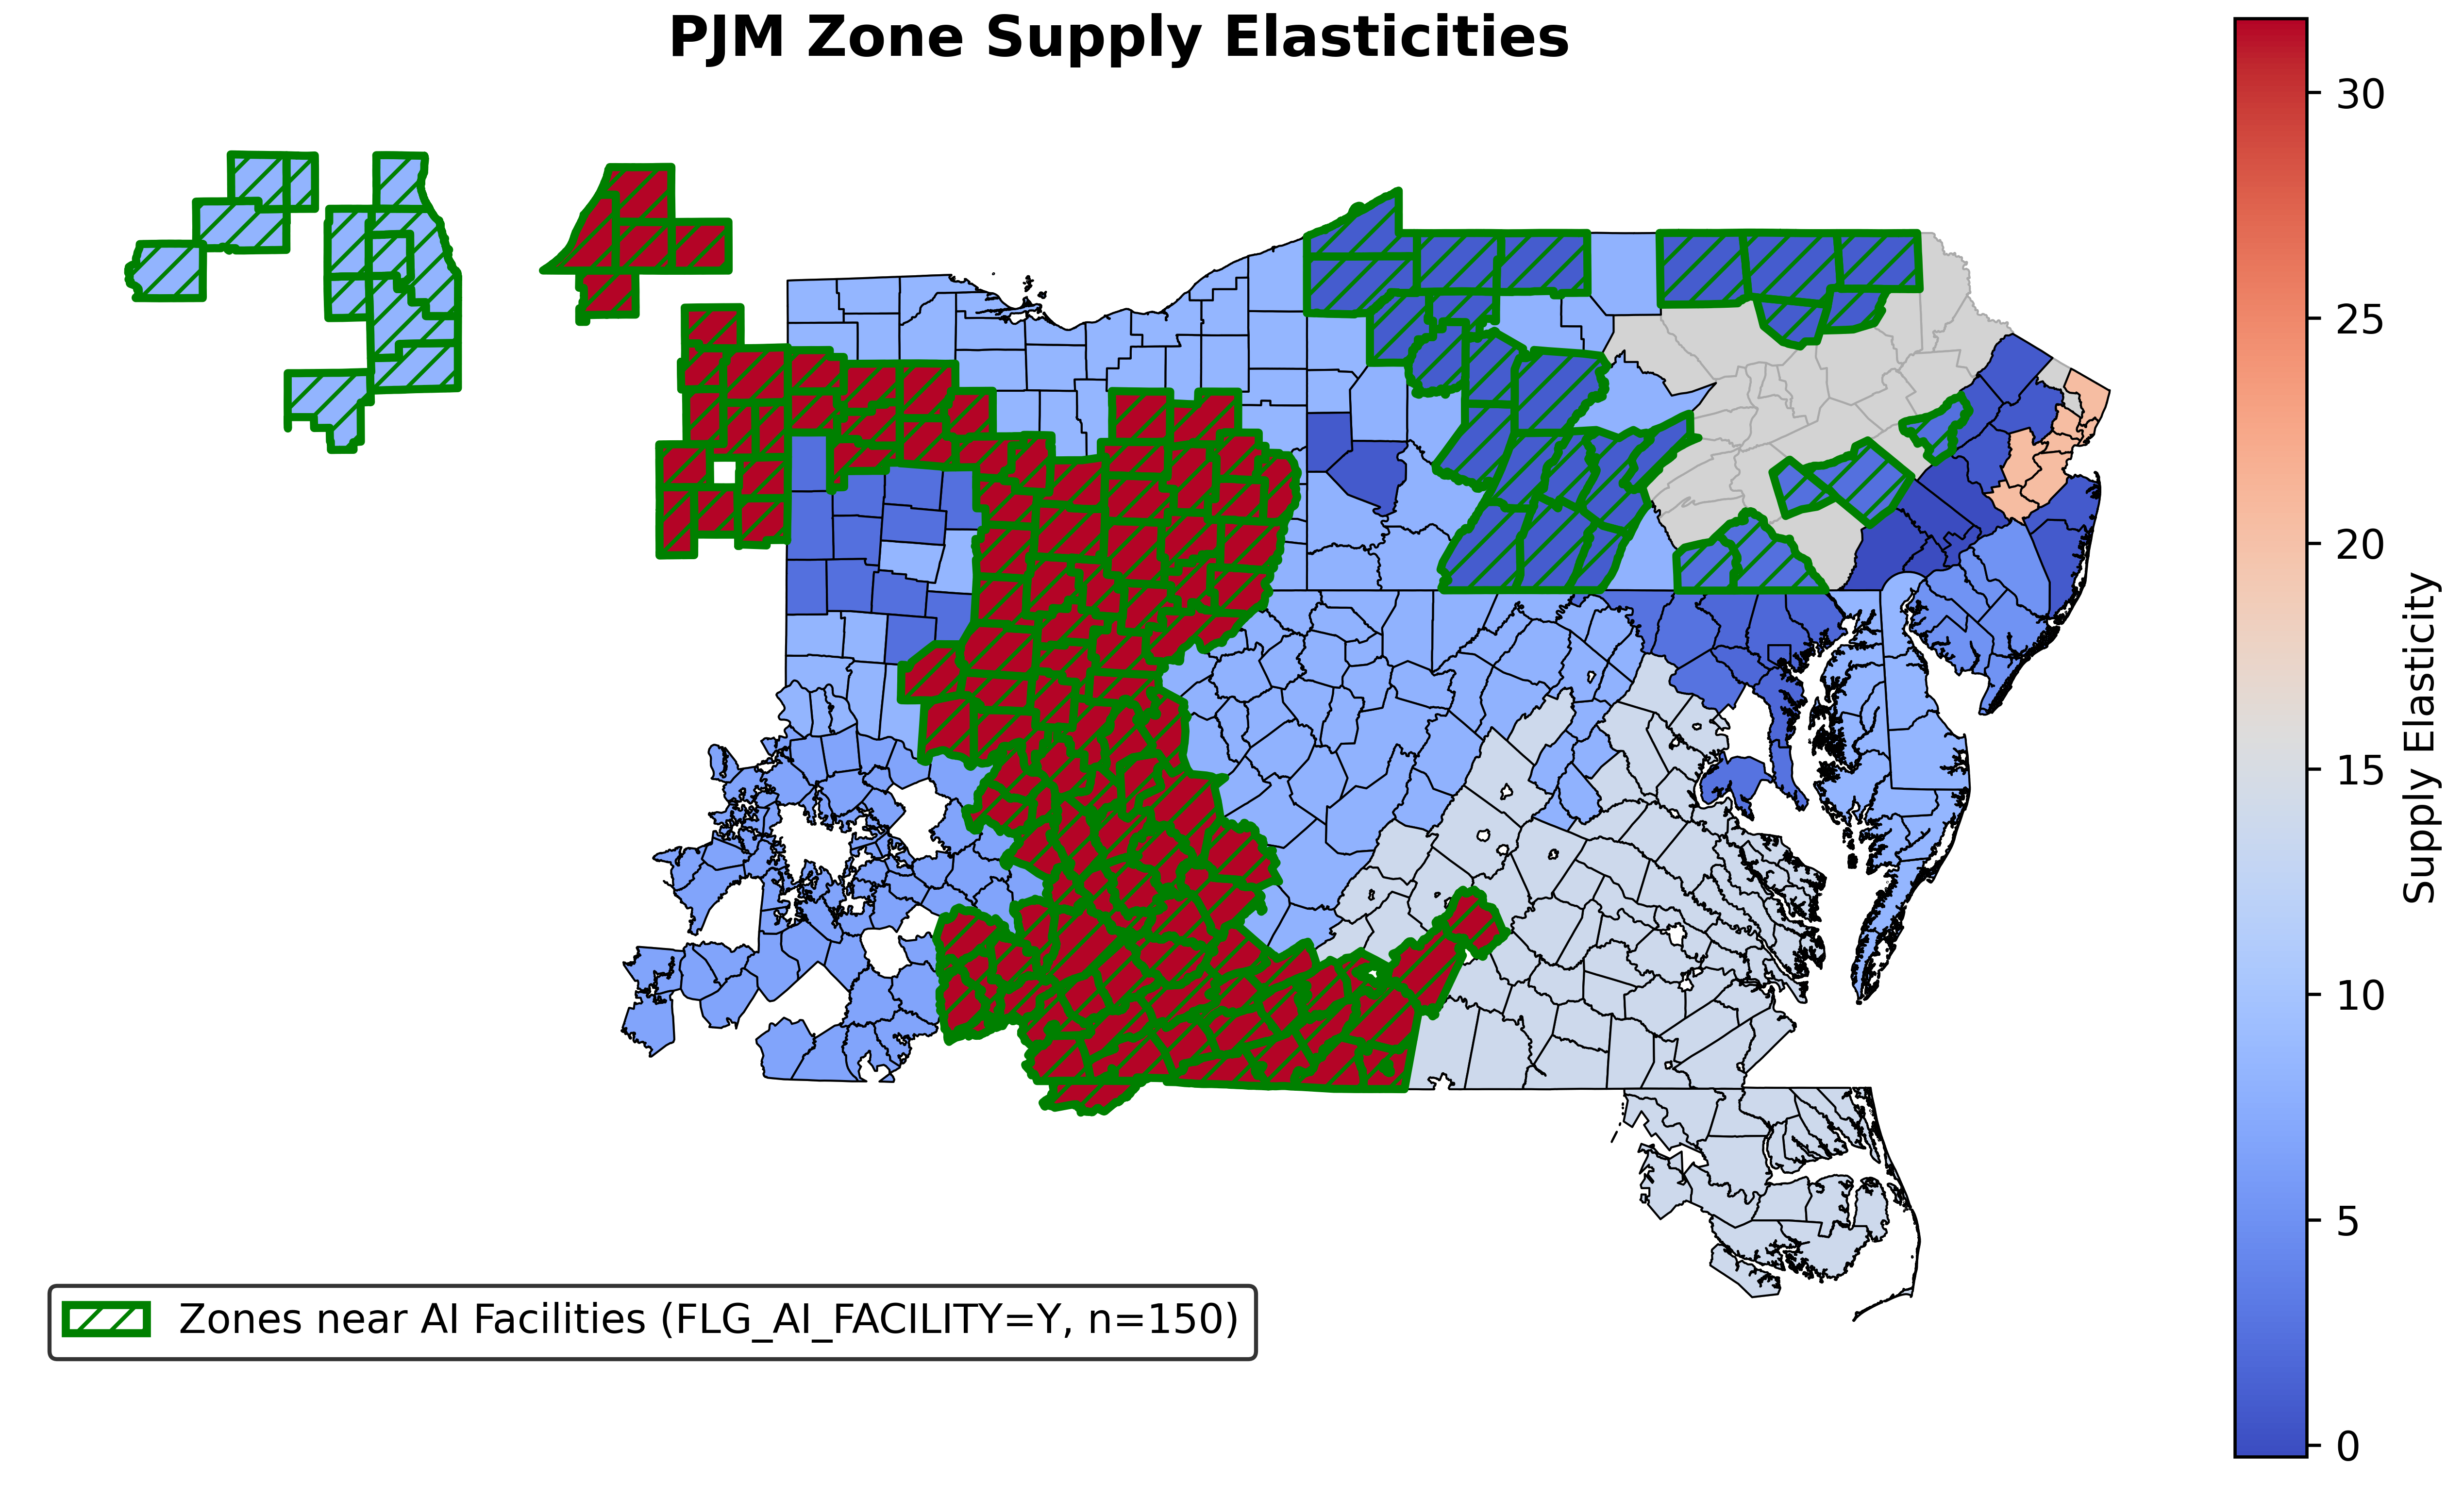
\includegraphics[width=0.5\linewidth]{Figures/pjm_ai_supply Elasticities.png}
    \caption{PJM Price Elasticity by Zone}
    \label{PJMPRiceElasticity}
\end{figure}

\subsection{Differences Between Power Quality and Demand Analyses}
\label{subsec:differences}

The power quality and fossil fuel demand analyses differ in geographic resolution and data structure due to the underlying data sources:

\begin{table}[t]
\centering
\resizebox{\columnwidth}{!}{%
\begin{tabular}{lcc}
\toprule
 & \textbf{Power Quality} & \textbf{Fossil Fuel Demand} \\
\midrule
Unit of observation & Utility-month & Generator-month \\
Geographic resolution & Utility service territory & Generator location \\
Treatment linkage & Utility contains AI data center & Generator near AI data center \\
Outcome source & Whisker Labs & EPA CEMS \\
Price endogeneity & Not modeled & IV with heat rate, gas price \\
\bottomrule
\end{tabular}
}
\caption{Summary of empirical designs}
\end{table}

These differences arise from data availability rather than conceptual distinctions. The power quality measures from Whisker Labs are aggregated to utility service territories, precluding finer spatial analysis. Generator-level EPA data permit more granular geographic matching, which we exploit for robustness analysis. The demand analysis additionally requires addressing price endogeneity because generation quantities reflect equilibrium outcomes in electricity markets; power quality indices are not directly determined by market clearing and thus do not require the same instrumentation strategy.

Despite these differences, we maintain a unified stacked DiD framework centered on model release dates for both analyses. This consistency facilitates comparison of effect dynamics across outcomes and provides a coherent narrative linking AI development activity to grid impacts.

\subsection{Additional Counterfactual Analysis}\label{Appendix:Counterfactuals}

\subsubsection{Training versus Inference Composition}

\textbf{Training-Inference Composition.} Third, we explore alternative compositions of AI workloads by selectively restricting channels in our model. By suppressing the training channel, we simulate power quality impacts under a scenario in which large-scale model training plateaus and the industry shifts toward an inference-dominant paradigm. Conversely, by suppressing the inference channel, we characterize outcomes under a shift toward primarily local, low-cost inference with reduced centralized training activity.

We explore how grid impacts would differ under alternative compositions of AI workloads.

\paragraph{Scenario: Inference-Dominant World.} If large-scale model training plateaus---perhaps due to diminishing returns to scale or compute constraints---while inference continues to grow with adoption, grid impacts would reflect primarily the inference channel.

\paragraph{Scenario: Training-Dominant World.} Conversely, if inference becomes predominantly local (on-device) while cloud resources are devoted primarily to training new models, impacts would concentrate in the training channel. Suppressing inference effects reduces additional power demand per hour per data center by significantly more than suppression of training. Figure~\ref{fig:channel_shutdown} provides insight into this relationship.

\begin{figure}[h]
    \centering
    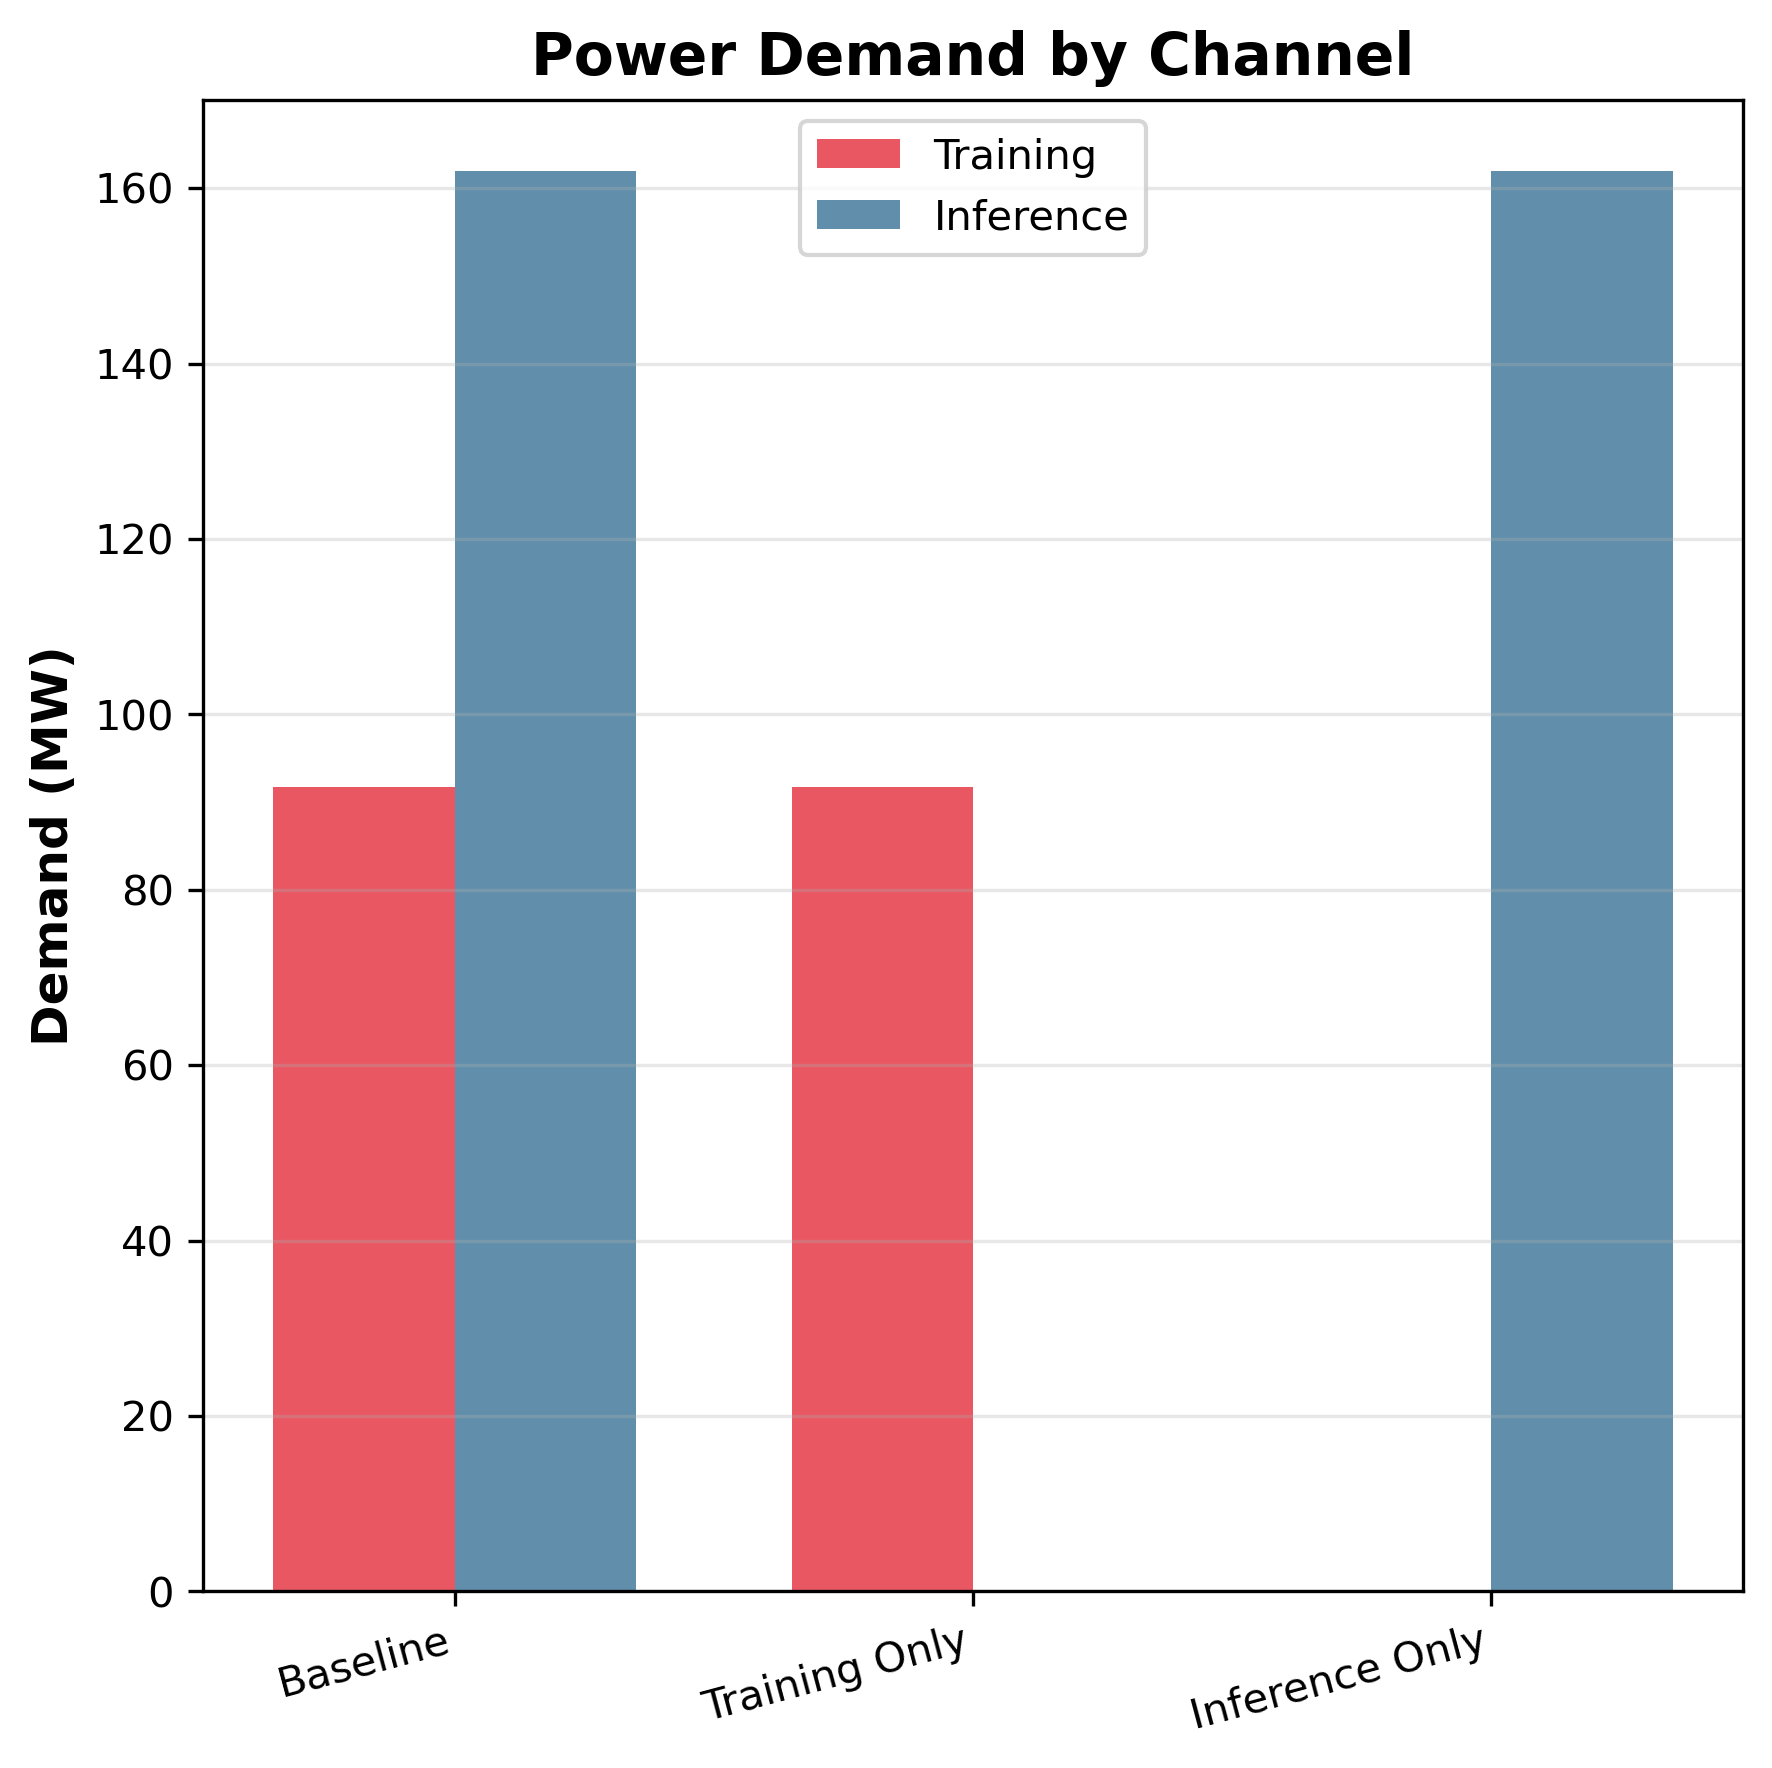
\includegraphics[width=0.5\linewidth]{Figures/channel_shutdown_analysis.png}
    \caption{Grid impacts under inference-only versus training-only scenarios.}
    \label{fig:channel_shutdown}
\end{figure}

\subsubsection{Efficiency Improvements}

\paragraph{Scenario: AI Efficiency Improvements.} Algorithmic efficiency represents a key lever for mitigating grid impacts. We calculate the potential impacts of efficiency gains, remaining agnostic about their source---improvements could come from both hardware and software advances related to AI training and inference. Figure~\ref{fig:efficiency_improvements} demonstrates how specific percentage-wise improvements in efficiency would affect the hourly demand coefficient. While a 40\% improvement in inference efficiency in our sample would lead to a 25\% reduction in total added demand, the same improvement in training efficiency would lead to only a 14\% reduction in demand.

\begin{figure}[h]
    \centering
    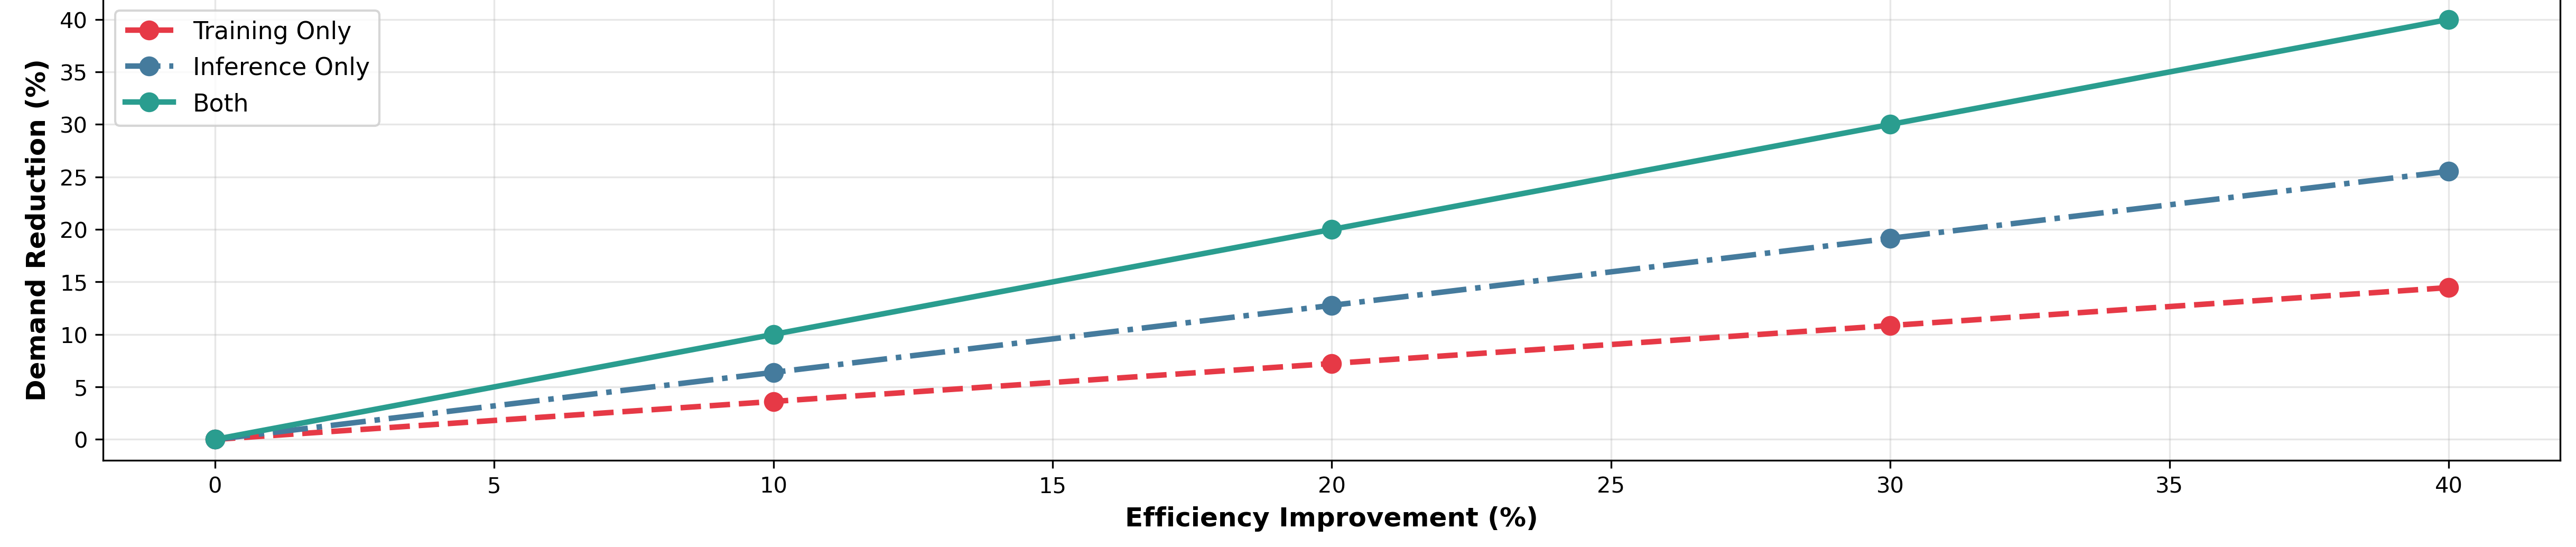
\includegraphics[width=0.5\linewidth]{Figures/comprehensive_counterfactual_summary.png}
    \caption{Reduction in power demand with efficiency improvements in training and inference.}
    \label{fig:efficiency_improvements}
\end{figure}

\subsubsection{Impacts of Agglomeration on Cost of System Outage}

\textbf{Impacts of Agglomeration on Cost of System Outage.} We examine the potential costs of agglomeration for cloud operators in terms of loss of service due to power outage. The concentration of AI workloads and AI data centers increases the strain in specific areas leading to greater costs on local grids and increasing the potential for long outages, which could lead to loss of service for cloud providers, which creates a significant revenue and reputational cost. These costs are bourne by data center operators themselves and so provide a non-socialized cost of data center impact on power grids that may justify spatial reorganization by the data center industry. We use publicly available estimates of the cost of recent losses of service by cloud platforms to tech companies to estimate these costs. 

Geographic concentration poses risks not only to the overall grid but also to cloud service reliability. The increased possibility of reliability events creates potential issues for cloud uptime and threatens continuous assurance of cloud services. As recently as 2022, a power failure in Ohio led to 3 continuous hours of downtime for Amazon Web Services US-EAST-2 \citep{Eisenberg2025AWSOutage}. Cloud losses were also associated with the blackouts during winter storm Uri in Texas. These outages impose costs on society as well as on hyperscalers in terms of lost revenue, damaged reputations, and security concerns.

We utilize documented estimates of outage costs from the literature (see Table~\ref{tab:outages} in Appendix Subsection ~\ref{app:outage_costs}) to estimate the economic costs to hyperscalers of increased reliability risk associated with data center concentration. We multiply the increase in the likelihood of a reliability event by the documented cost associated with a cloud outage of the length of a reliability event. We find that a shift to an edge-computing scenario as detailed above would lead to significant reliability-related savings for hyperscalers in our sample based only on treated models. Similarly, a full implementation of on-site colocated generation would lead to a total average decrease in the number of reliability events in data center utility areas of approximately .17 per month. This means that the number of reliability events per year making the IID assumption decreases by 2.04 events per year. We assume that a significant power outage that leads to a cloud outage has a median duration of 21 hours matching our data with a median cost per hour of 19.2 million. We further conservatively assume that a significant reliability event near a data center has a probability of leading to a cloud outage of 5\%. The implied reliability savings associated with on-site generation are thus \textbf{41 million} accrued to the hyperscaler. This is a significant financial argument for hyperscalers to work towards improved reliability.

\subsection{Treatment Definition and Data Linkage}
\label{subsec:treatment}

Our treatment relies on linking AI model releases to geographic regions through a chain of observable connections: models to companies, companies to data center locations, and data center locations to electricity service territories. We describe each link and its limitations.

\subsubsection{Identifying AI Data Centers}

We leverage a recently released variable from Aterio that directly classifies data centers by their primary use case, including a designation for AI-focused facilities. This classification improves upon prior approaches that treated all data centers homogeneously, as AI workloads---particularly large-scale model training---exhibit distinct load profiles characterized by sustained high utilization and substantial power draws that differ markedly from traditional cloud computing or storage operations.

We link data centers to electricity service territories at two geographic resolutions:
\begin{itemize}
    \item \textbf{Utility service territory:} For power quality analysis, we match AI data centers to retail electric utility boundaries. A utility is designated as treated if at least one AI data center operates within its service territory.
    \item \textbf{Generator proximity:} For fossil fuel demand analysis, we match data centers to generators by picking generators within a 20-mile radius of an in-sample data center. This finer resolution exploits the greater spatial granularity of EPA generator-level data.
\end{itemize}

\subsubsection{Linking Models to Data Centers}

We construct a crosswalk from AI model releases to data center locations through company ownership. For each major model release in our sample, we identify the developing company and link to all AI-classified data centers operated by or contracted to that company. 

\paragraph{Identifying Assumption and Limitations.} Our approach assumes that training and inference activity for a given model occurs at data centers associated with the releasing company. This assumption is imperfect for several reasons:
\begin{enumerate}
    % \item We do not observe the specific facility where training occurred. A company with multiple data centers may concentrate training at a subset of locations.
    \item Training may occur at third-party cloud facilities not captured in our data center inventory.
    \item Inference workloads may be distributed across facilities differently than training workloads.
\end{enumerate}

We interpret our estimates as capturing the \textit{average} effect across a company's AI data center footprint, which represents a lower bound on the localized effect at the actual training site if activity is concentrated, or an upper bound if we misattribute activity to facilities that were not involved. We probe robustness to this measurement error through several approaches described in Section~\ref{subsec:robustness}.

For a subset of models where public information permits more precise dating, we supplement our treatment timing with verified training and inference windows:

\subsection{Quantifying Costs of Loss of Cloud Services}\label{app:outage_costs}

Table~\ref{tab:outages} presents cloud service outages filtered to include only (1) incidents related to power infrastructure failures, or (2) incidents with verified financial impact estimates from cited sources. This dataset supports analysis of agglomeration costs for cloud operators arising from power grid strain and service disruption.

\begin{table}[t]
\centering
\scriptsize
\caption{Cloud Outages: Power-Related and Documented Costs (2021--2024)}\label{tab:outages}
\begin{tabular}{@{}lccrc@{}}
\toprule
Provider & HS & Pwr & Hrs & Cost \\
\midrule
% ERCOT~\cite{lee2022texas} & 0 & 1 & 71 & \$130B\textsuperscript{a} \\
OVHcloud~\cite{uptime2021ovh} & 0 & 1 & 288 & \euro10M\textsuperscript{b} \\
Fastly~\cite{fastly2021postmortem} & 0 & 0 & 1 & \$34M\textsuperscript{c} \\
GCP~\cite{dcd2022gcplondon} & 1 & 1 & 18 & --- \\
AWS~\cite{aws2022useast2} & 1 & 1 & 3 & --- \\
GCP~\cite{dck2022gcpiowa} & 1 & 1 & 4 & --- \\
Rackspace~\cite{rackspace2023sec} & 0 & 0 & 504 & \$35M\textsuperscript{d} \\
Alibaba~\cite{scmp2022alibaba} & 0 & 1 & 24 & --- \\
GCP~\cite{register2023gcpparis} & 1 & 1 & 336 & --- \\
CrowdStrike\textsuperscript{e}~\cite{parametrix2024crowdstrike} & 0 & 0 & 72 & \$5.4B\textsuperscript{f} \\
Alibaba~\cite{dcd2024alibabafire} & 0 & 1 & 144 & --- \\
GCP~\cite{register2024gcpfrankfurt} & 1 & 1 & 13 & --- \\
Azure~\cite{statusgator2024azure} & 1 & 1 & 6 & --- \\
\bottomrule
\end{tabular}

\vspace{0.3em}
\raggedright
\tiny
\textit{Notes:} HS = Hyperscaler (AWS/Azure/GCP). Pwr = Power/electrical/cooling/fire. Hrs = Duration.
\textsuperscript{a}TX total; \$4.3B direct.
\textsuperscript{b}Lawsuit awards.
\textsuperscript{c}Amazon only.
\textsuperscript{d}Revenue + remediation.
\textsuperscript{e}Third-party; affected Azure.
\textsuperscript{f}Fortune 500; insured \$0.5--1.1B.
\end{table}

\vspace{1em}
\noindent\textbf{Notes:}
\begin{enumerate}
    % \item[a.] Total economic impact estimate for Texas; \$4.3B in direct power costs per Dallas Fed.
    \item[b.] Lawsuit settlements; individual awards ranged \euro100K--\euro154K.
    \item[c.] Estimated Amazon revenue loss alone during 1-hour outage.
    \item[d.] Combines \$30M annual Hosted Exchange revenue loss plus \$5M remediation costs per SEC filings.
    \item[e.] Third-party vendor incident primarily affecting Microsoft Azure customers.
    \item[f.] Fortune 500 companies only; insured losses estimated \$540M--\$1.08B by Parametrix.
\end{enumerate}

\vspace{1em}
\noindent\textbf{Variable Definitions:}
\begin{itemize}
    \item \textbf{Hyperscaler}: Binary indicator (1 = AWS, Azure, or GCP; 0 = other providers).
    \item \textbf{Power}: Binary indicator (1 = outage caused by or related to power infrastructure, electrical systems, cooling failures, or fires; 0 = software, network, or security causes).
    \item \textbf{Duration}: Hours from incident onset to service restoration; ``+'' indicates ongoing recovery beyond initial resolution.
\end{itemize}

\subsubsection{Instrumental Variables Specification}\label{IVDetails}

The learned DiD coefficients capture the relationship between AI model releases and generator output, but this relationship may be confounded by supply-side shocks. For example, if AI model releases coincide with changes in natural gas prices or generator availability that independently affect electricity production, our estimates would conflate demand-side and supply-side effects. To isolate the demand-side effects, we instrument for electricity prices using the interaction of generator-level heat rates and regional natural gas prices. This instrumentation strategy exploits cross-sectional variation in generators' fuel efficiency: conditional on natural gas price movements, generators with higher heat rates (lower efficiency) face larger marginal cost shocks, allowing us to trace out the demand curve.

\paragraph{First-Stage and Structural Estimates.} The first stage regresses electricity prices on the heat rate--gas price interaction. The structural equation then uses predicted prices to estimate price responsiveness. The estimated price elasticity from the structural equation is 0.135 (SE = 0.013, p < 0.0001), indicating economically meaningful and precisely estimated demand responsiveness. As a specification check, we estimate the first stage separately for each of 5 model-specific regressions; the mean price coefficient is $-0.331$ (SD = 0.005, range: $-0.336$ to $-0.323$). The tight clustering of estimates across specifications suggests stable demand elasticity across AI model events and supports the validity of our instrumentation strategy.

\subsubsection{Interpretation and Caveats for Price Analysis}\label{appendix:Caveats}

These calculations provide ballpark estimates of how AI-induced demand shifts translate to wholesale price changes. Several caveats apply:
\begin{enumerate}
    \item The supply elasticity varies across regions and time periods; our estimates represent averages that mask considerable heterogeneity.
    \item If AI workloads can be temporally shifted to off-peak hours when supply is more elastic, price impacts would be smaller than our estimates suggest.
    \item We do not model transmission constraints, which may amplify local price effects in congested areas near data centers.
\end{enumerate}

\subsection{Wholesale-to-retail Passthrough Estimates}\label{WholesaleRetailPassthrough}

\begin{table}[H]
\centering
\caption{Wholesale-to-Retail Price Pass-Through in Deregulated Markets}
\label{tab:passthrough}
\scriptsize
\begin{tabular}{@{}llcc@{}}
\toprule
\textbf{Study} & \textbf{ISO} & \textbf{PT} & \textbf{Class} \\
\midrule
\multicolumn{4}{@{}l}{\textit{Panel A: Wholesale $\to$ Retail Pass-Through}} \\
\addlinespace[0.3em]
\citet{defeuilley2023pennsylvania} & PJM (PA) & 0.53 & Res. (EDC) \\
\citet{defeuilley2023pennsylvania} & PJM (PA) & 0.56 & Res. (EGS) \\
% \citet{tsai2025ohio} & PJM (OH) & ---$^a$ & Res. \\
\citet{brown2020texas} & ERCOT & 0.43--0.47 & Res. \\
\citet{mackay2024wholesale} & Multi & $\approx$1.0$^b$ & All \\
\midrule
\multicolumn{4}{@{}l}{\textit{Panel B: Demand Elasticity (Residential)}} \\
\addlinespace[0.3em]
\citet{deryugina2020longrun} & PJM (IL) & $-0.09$ & SR (1 mo.) \\
\citet{deryugina2020longrun} & PJM (IL) & $-0.27$ & MR (2 yr.) \\
\citet{deryugina2020longrun} & PJM (IL) & $-0.35$ & LR (10 yr.) \\
\bottomrule
\end{tabular}

\vspace{0.3em}
\raggedright
\scriptsize
\textit{Notes:} PT = pass-through coefficient. EDC = Electric Distribution Company; EGS = Electric Generation Supplier. SR/MR/LR = short/medium/long-run. \\
% $^a$Complex mechanism; volatility inflates auction premia. \\
$^b$Long-run; \$9.59/MWh cost $\to$ \$8.81/MWh retail.
\end{table}

\subsubsection{On-site Generation Estimation Details}
% \nb{move to appendix}
Data centers increasingly deploy on-site generation to reduce grid dependence. Our data center inventory identifies 87 facilities with on-site power generation capability and 12,401 without. We test whether on-site capacity moderates estimated effects by interacting treatment with on-site status in the utility-level strict DiD specification. Results indicate that on-site generation substantially mitigates measured grid impacts.

\begin{table}[h]
\centering
\caption{Power Quality Effects by On-site Generation Status}
\label{tab:btm_effects}
\resizebox{\columnwidth}{!}{% % This scales the table to fit
\begin{tabular}{lcccc}
\toprule
Outcome & With On-site & W/O On-site & Diff. & Interpretation \\
\midrule
CPQI & $-0.122$ & $+0.228$ & $-0.350$ & On-site reduces grid stress \\
% THD & $+0.120$ & $-2.174$ & $+2.294$ & BTM reduces harmonic distortion \\
\bottomrule
\end{tabular}%
}
\begin{flushleft}
\footnotesize\textit{Notes:} All coefficients significant at $p < 0.001$. CPQI: Consumer Power Quality Index.
\end{flushleft}
\end{table}

The sign reversal for CPQI is notable: data centers \textit{with} on-site generation are associated with improved power quality (negative coefficient), while those \textit{without} on-site generation are associated with deterioration (positive coefficient). This heterogeneity suggests that on-site generation absorbs demand spikes that would otherwise propagate to the grid, and implies that aggregate grid impacts understate total AI energy consumption. It should be noted that all large AI data centers in our most conservative sample had on-site generation. This may imply that our estimates of the impacts of on-site generation are exaggerated by a differential sample.

%\nb{Dana, why dont have we the parallel trends validation for power quality as well?}


\subsection{Additional Robustness Checks}\label{App:AdditionalRobustnessChecks}

% \subsubsection{Anomaly detection}

\subsubsection{Robustness Checks}
We test result robustness by varying treated population definitions, estimating specifications with alternative geographic boundaries to confirm consistency. This demonstrates findings reflect genuine causal impacts rather than arbitrary boundary choices. While we lack data on which models run at specific centers, our DiD methodology accounts for this by using publication dates as exogenous treatment, utilizing minimal geographic and temporal treatment windows. We plan robustness checks restricting treatment to larger data centers most likely involved in AI training. To verify treatment effects aren't noise-related, we include appendix robustness checks with randomized treatment dates as additional evidence that effects relate to model releases.

\subsubsection{Treatment Intensity}

Rather than binary treatment indicators, we estimate a continuous treatment intensity specification using total electricity demand (MWh) as the treatment variable. The significant coefficient (p < 0.001; THD: $+0.00018$, p < 0.001) indicate dose-response relationships: larger electricity loads are associated with larger power quality changes.

\subsubsection{Confirmed Locations and Verified Dates}

We re-estimate our main specifications using stricter treatment definitions. The confirmed-location analysis restricts treatment to facilities with precisely geocoded training locations (mean effect: 74.19 MWh). The verified-date analysis uses API release timing rather than publication dates from the Epoch database (mean effect: 63.20 MWh). Both analyses corroborate our main findings with expected attenuation from the more conservative treatment definitions.



\end{document}
